% Load the kaobook class
\documentclass[
  french,english,
	fontsize=10pt, % Base font size
	twoside=true, % Use different layouts for even and odd pages (in particular, if twoside=true, the margin column will be always on the outside)
	open=any, % If twoside=true, uncomment this to force new chapters to start on any page, not only on right (odd) pages
	secnumdepth=2, % How deep to number headings. Defaults to 1 (sections)
  numbers=enddot,
]{kaobook/kaobook}

% Choose the language
\usepackage{babel} % Load characters and hyphenation
\usepackage[english=british]{csquotes}	% English quotes

% Load packages for testing
\usepackage{blindtext}
%\usepackage{showframe} % Uncomment to show boxes around the text area, margin, header and footer
%\usepackage{showlabels} % Uncomment to output the content of \label commands to the document where they are used

% Load the bibliography package
\usepackage[style=alphabetic,maxbibnames=99]{kaobook/kaobiblio}
\DefineBibliographyExtras{french}{\restorecommand\mkbibnamefamily} %To have consistent citations between French and English text
\addbibresource{biblio.bib} % Bibliography file

% Load my own packages
\usepackage{styles/layout}
\usepackage{styles/macros}
\usepackage{styles/alectryon-minted}

% Load mathematical packages for theorems and related environments
\usepackage[background=black!5,boxed]{kaobook/kaotheorems}

% Load the package for hyperreferences
\usepackage{kaobook/kaorefs}

%\includeonly{gradual-dependent}

\graphicspath{{./figures/}} % Paths where images are looked for

%\makeindex[columns=3, title=Alphabetical Index, intoc] % Make LaTeX produce the files required to compile the index

% \knowledgestyle*{notion}{style={color=black!80!},intro style={color=black!80!,emphasize}}

\knowledgestyle{notion}{color=black}
\knowledgestyle{notion intro}{color=LightOrange,emphasize}
\knowledgedirective*{notion}{autoref,style=notion,intro style=notion intro}

\knowledgestyle{ignore intro}{color=LightOrange,emphasize}
\knowledgedirective*{ignore}{intro style=ignore intro}

\knowledgedirective*{title}{}


%Chapter 1

\knowledge{ignore}
  | type
  | types

\knowledge{notion}
  | type dépendant
  | types dépendants
  | théorie des types dépendants
  | dépendant@typ
  | dépendants@typ

\knowledge{notion}
  | assistant à la preuve
  | assistants à la preuve

\knowledge{notion}
  | Coq

\knowledge{notion}
  | Agda

\knowledge{notion}
  | correspondance de Curry-Howard

\knowledge{notion}
  | Gallina

\knowledge{notion}
  | noyau

\knowledge{notion}
  | critère de De Bruijn

\knowledge{notion}
  | MetaCoq

\knowledge{notion}
  | bidirectionnel
  | typage bidirectionnel

\knowledge{notion}
  | graduel
  | graduels
  | typage graduel
  | type graduel
  | types graduels

% Chapter 2

\knowledge{notion}
  | dependent type

\knowledge{notion}
  | Curry-Howard correspondence

\knowledge{notion}
  | kernel

\knowledge{notion}
  | De Bruijn’s criterion

\knowledge{notion}
  | proof assistant

% Chapter 3

% Section 3.2
\knowledge{notion}
  | Calculus of Constructions
  | CCω

\knowledge{title}
  | CCω@tit
  | Calculus of Constructions@tit

\knowledge{notion}
  | CIC
  | Calculus of Inductive Constructions

\knowledge{title}
  | CIC@tit
  | Calculus of Inductive Constructions@tit

\knowledge{notion}
  | Polymorphic, Cumulative Calculus of Inductive Constructions
  | PCUIC

\knowledge{title}
  | PCUIC@tit

\knowledge{notion}
  | α-equality
  | α-equal 

\knowledge{notion}
  | Church-style

\knowledge{notion}
  | Curry-style

\knowledge{notion}
  | universe level
  | universe levels
  | level
  | levels

\knowledge{notion}
  | typical ambiguity


% Section 3.3 
\knowledge{notion}
  | conversion

\knowledge{notion}
  | typed conversion
  | Typed conversion
  | typed@conv

\knowledge{notion}
  | untyped conversion
  | Untyped conversion
  | untyped@conv

\knowledge{notion}
  | Pure Type Systems
  | PTS

\knowledge{notion}
  | declarative conversion
  | Declarative conversion
  | declarative@conv
  | conversion@decl

\knowledge{notion}
  | algorithmic conversion
  | algorithmic@conv

\knowledge{notion}
  | reduction

\knowledge{notion}
  | top-level reduction
  | Top-level reduction
  | top-level reductions
  | top-level@red

\knowledge{notion}
  | one-step reduction
  | one-step@red

\knowledge{notion}
  | weak-head reduction
  | weak-head@red

\knowledge{notion}
  | full reduction
  | full@red

% Section 3.4
\knowledge{notion}
  | stability under renaming
  | Stability under renaming
  | stable under renaming

\knowledge{notion}
  | weakening
  | Weakening

\knowledge{notion}
  | stability under substitution
  | Stability under substitution
  | stable under substitution

\knowledge{notion}
  | conditional stability under renaming
  | Conditional stability under renaming


\knowledge{notion}
  | strengthening
  | Strengthening

\knowledge{notion}
  | uniqueness of types up to
  | uniqueness of types
  | Uniqueness of types
  | uniqueness@typ

\knowledge{notion}
  | validity
  | Validity

\knowledge{notion}
  | Subject reduction
  | subject reduction
  | preservation

\knowledge{notion}
  | injectivity of function types
  | Injectivity of function types
  | injectivity of type constructors

\knowledge{notion}
  | confluence
  | Confluence

\knowledge{notion}
  | normal form
  | normal forms

\knowledge{notion}
  | neutral form
  | neutral forms
  | neutral
  | neutrals

\knowledge{notion}
  | canonical form
  | canonical forms

\knowledge{notion}
  | progress
  | Progress

\knowledge{notion}
  | accessible
  | Accessibility

\knowledge{notion}
  | Normalization
  | normalization
  | normalizing

\knowledge{notion}
  | logical consistency
  | logically consistent
  | Logical consistency

\knowledge{notion}
  | canonicity
  | Canonicity

% Section 3.5 
\knowledge{notion}
  | inductive type
  | inductive types

\knowledge{notion}
  | boolean
  | booleans

\knowledge{notion}
  | constructor
  | constructors

\knowledge{notion}
  | recursor
  | recursors
  | induction principle

\knowledge{notion}
  | scrutinee
  | predicate
  | branches

\knowledge{notion}
  | fully applied

\knowledge{notion}
  | indexed@ind
  | indexed inductive type
  | indexed inductive types

\knowledge{notion, text ={CIC\textsuperscript{-}}}
  | CIC-


% Section 3.6
\knowledge{notion}
  | cumulativity

\knowledge{notion}
  | α-pre-order

\knowledge{notion}
  | impredicativity

\knowledge{notion}
  | proof irrelevance

\knowledge{notion}
  | local definitions
  | local definition

\knowledge{notion}
  | environment

\knowledge{notion}
  | guard condition

\knowledge{notion}
  | record type
  | record types
  | record@type

\knowledge{notion}
  | projection
  | projections

\knowledge{notion}
  | co-inductive type
  | co-inductive types

% Bidirectional part

\knowledge{notion}
  | mode
  | modes
  | subject
  | inputs
  | input
  | outputs
  | output

\knowledge{notion}
  | undirected typing
  | undirected@typ

% Chapter 4

\knowledge{notion}
  | well-formed
  | well-typed

\knowledge{notion}
  | inference

\knowledge{notion}
  | checking

\knowledge{notion}
  | Matita

\knowledge{notion}
  | boundary

\knowledge{notion}
  | constrained inference

\knowledge{notion}
  | full

\knowledge{notion}
  | type-level enforcing

\knowledge{notion}
  | Correctness
  | correctness@bidir
  | correct@bidir
  | Correctness@bidir

\knowledge{notion}
  | Completeness
  | completeness@bidir
  | complete@bidir
  | Completeness@bidir

% Chapter 5

\knowledge{notion}
  | principal type
  | principal@type

% MetaCoq

\knowledge{notion}
  | GitHub

\begin{document}

%----------------------------------------------------------------------------------------
%	BOOK INFORMATION
%----------------------------------------------------------------------------------------

% \titlehead{Document Template}
\title[Bidirectional Typing in the Calculus of Inductive Constructions]{Bidirectional Typing in the Calculus of Inductive Constructions}
\subtitle{Doctoral Thesis}
\author[M. Lennon-Bertrand]{Meven Lennon-Bertrand}
\date{\today}
% \publishers{An Awesome Publisher}

%----------------------------------------------------------------------------------------

\frontmatter % Denotes the start of the pre-document content, uses roman numerals

%----------------------------------------------------------------------------------------
%	COPYRIGHT PAGE
%----------------------------------------------------------------------------------------

\makeatletter
\uppertitleback{\@titlehead} % Header

\lowertitleback{
	% \textbf{Disclaimer} \\
	% You can edit this page to suit your needs. For instance, here we have a no copyright statement, a colophon and some other information. This page is based on the corresponding page of Ken Arroyo Ohori's thesis, with minimal changes.
	
	% \medskip
	
	% \textbf{No copyright} \\
	% \cczero\ This book is released into the public domain using the CC0 code. To the extent possible under law, I waive all copyright and related or neighbouring rights to this work.
	
	% To view a copy of the CC0 code, visit: \\\url{http://creativecommons.org/publicdomain/zero/1.0/}
	
	% \medskip
	
	% \textbf{Colophon} \\
	% This document was typeset with the help of \href{https://sourceforge.net/projects/koma-script/}{\KOMAScript} and \href{https://www.latex-project.org/}{\LaTeX} using the \href{https://github.com/fmarotta/kaobook/}{kaobook} class.
	
	% \medskip
	
	% \textbf{Publisher} \\
	% First printed in May 2019 by \@publishers
}
\makeatother

%----------------------------------------------------------------------------------------
%	DEDICATION
%----------------------------------------------------------------------------------------

\dedication{\raggedleft\emph{À Tangi,\\
Parce que je sais que tu aurais été le premier à te réjouir avec moi de là où j’en suis arrivé…
et le premier à te moquer de moi pour me garder les pieds sur terre.}}

% \dedication{
% 	% The harmony of the world is made manifest in Form and Number, and the heart and soul and all the poetry of Natural Philosophy are embodied in the concept of mathematical beauty.\\
% 	% \flushright -- D'Arcy Wentworth Thompson
% }

%----------------------------------------------------------------------------------------
%	OUTPUT TITLE PAGE AND PREVIOUS
%----------------------------------------------------------------------------------------

\includepdf[pages=1]{../MathSTICTemplate/main.pdf}

% Note that \maketitle outputs the pages before here
\maketitle

%----------------------------------------------------------------------------------------
%	PREFACE
%----------------------------------------------------------------------------------------

\begingroup

  %in the header, chapters start on any page to avoid too many blank pages
  \let\cleardoublepage\clearpage
  \pagelayout{margin}

\addchap{Abstract}

This thesis broadly considers the question of giving a bidirectional treatment of the
Calculus of Constructions (CIC), which underpins the proof assistant \kl{Coq}, under
three different angles corresponding to its three parts.

It first considers the question of giving a bidirectional account of CIC
from a theoretical point
of view. It contains the exposition of such a bidirectional presentation of CIC, with the
general discipline that led to it. Follow a proof of equivalence between this presentation
and the standard one. This equivalence is then used to establish properties of CIC that
are hard to obtain in the standard setting: existence of principal types, and strengthening.

The second part sets on to formalize the idea of the first one,
in the setting of the \kl{MetaCoq} project,
which aims at formalizing the meta-theory CIC in \kl{Coq}, and to implement
a kernel that is proven correct and complete. The formalized bidirectional structure supplies
an intermediate between the high-level specification and the algorithm, which is key in
order to prove that the kernel is complete.

Finally, the last part considers the question of designing an extension of CIC incorporating
ideas from gradual typing, with the aim of bringing more flexibility to development in \kl{Coq}.
The bidirectional structure is once again valuable, as the characteristics of gradual typing
– in particular the way it relaxes conversion – 
make it impossible to base the extension on the standard presentation of CIC.

\addchap{Acknowledgments}

I wouldn’t have got halfway to the end of this thesis without the many great people around me,
so let me try and thank them here for all they have brought me.

Obviously, the one person this thesis owes the most to is my advisor Nicolas. I feel extremely
lucky to have had the possibility to run free and do my things, while still knowing that
he was in the next office with an open door whenever I got an issue.
I am proud that I can call myself his student.

Beyond Nicolas, I am very honoured that my jury members accepted to be part of it.
Neel and Conor,
because of their deep knowledge about bidirectional typing and programming language
theory in general.
Herman, because my year in Nijmegen has been an important one for where I am today.
Christine and Hugo, because they shaped the great tool that \kl{Coq} is today; and, for Hugo,
because he was the one who introduced me both to \kl{Coq} and to research.
Jesper, because I have a great respect his work on \kl{Agda}.
I hope there are still many pages to
write in the collaboration between our two close but yet subtly different worlds.
Matthieu, because his work on \kl{MetaCoq} is impressive, and he still is kind enough to
let me leave him discharge on him my ugliest lemmas.
Finally, Assia, because I admire both her achievements and her genuine humanity.

During these three and a half years, I have learned so much from the researchers around me,
and I am very grateful for that.
From Pierre-Marie, that you should not be afraid to stand by your ideas.
From Assia, that this does not mean you have to crush others,
but that you can instead learn a great deal from them, exactly because they took another path.
From Guillaume, that there are some non-negotiable values in academia that you cannot just 
ignore.
From Guilhem, I hopefully learned a bit about teaching. Thanks for helping me navigate the
meanders of the university and for trusting me with your exercise sessions.
From Matthieu, I learned most of what I know about another kind of meanders,
those of \kl{Coq} and formalization.
Éric taught me that having a solid technique
is only useful if readers get that far in your paper, and showed me how to achieve that.

But Gallinette is not only permanent researchers, and I learned an equally great deal from
my \textit{senpais}. Marie and Étienne came up with the brilliant idea of the Quésaco seminars.
Yannick still patiently answer my random questions, even after so many of them.
Théo guided me through the intricacies of the PhD, which is no small feat.
Loïc does not really fit in the \textit{senpai} category,
after all of the two thesis siblings I am
the one coming out first. Still, I learned a lot with him, from precious insight on
normalization to painting beautiful banners.
Good luck with your own writing, and see you on the other side!
Last but not least, Kenji taught me just too many things to be all recorded here.
I’ll miss our random but always worthwhile exchanges between computer screens and your
valuable ideas on dependent types and vegetables alike.

Learning is nice, but it’s not everything. Happily, the Gallinette members are not just
cool researchers, they are also wonderful people, and it’s been an immense pleasure to work
in that team. Thanks to all those I have already mentioned and to
Pierre (Vial), Maxime, Simon, Matthieu (Piquerez), Ambroise, Xavier, Martin, Enzo,
Pierre (Benjamin? Giraud? How do I cite you?), Hamza, Chris, Gaëtan
for the seminars, coffee discussion, corridor talks, online chats, beer disputes,
and all the other conversations. A special acknowledgment to Ambroise for thanking me in
advance in his thesis, the prophecy has been accomplished.
Following this now established tradition, I hereby thank in advance
Martin, Enzo, Pierre, Hamza and Chris for thanking me in their own theses when the time comes.
Best of luck to get there.
Another special thanks to those who proofread this thesis even with the rushy calendar,
and especially to Martin who found the courage to go through all of it. You made it much
better than it was.
And let me not forget Anne-Claire, who kindly watches over our unruly lot.

\selectlanguage{french}

Au-delà de Gallinette, je me dois aussi de mentionner les doctorant·e·s du LS2N.
Entre le Covid et la rédaction, je n’ai que trop peu profité d’eux, mais quelle
une chouette équipe ! Merci aussi à toute l’équipe des CHATS, Sylvain, Bertrand, Rémi,
Brigitte, Audrey, Marianne, Baptiste, Mélanie, et tou·te·s les profs et élèves du lycée
Michelet. Ces trois années d’art et de sciences n’ont pas exactement été de tout repos,
mais j’ai été très heureux de partager un peu de mon enthousiasme pour
les mathématiques et l’informatique, et de tant recevoir en retour.
J’ai également eu le plaisir de faire partie de l’éphémère collectif des précaires à l’hiver
2020, presque aussi vite dispersé qu’il s’est formé.
% Où que le vent de la lutte vous
% porte, j’espère que vous continuerez à semer des petites graines de révolte.
Merci à eux et à tous les autres qui luttent pour faire de l’université et
du monde des endroits un peu meilleurs.

\selectlanguage{english}

These pandemics years have not exactly been the best for exchanges. Yet, I feel very
fortunate to be part of the thriving proof assistants and types communities. Thanks for
all the online questions, answers and discussions, for giving nice talks and listening to
mine. Hope to finally meet you all in person soon. And thanks to Andrej for giving me the
occasion to have the first (!) scientific trip of my PhD in Ljubljana.

\selectlanguage{french}

Je n’aurais jamais pu arriver là où j’en suis sans les nombreux·ses enseignant·e·s
qui ont croisé ma longue route de la maternelle au master. Ils et elles ont su nourrir
ma curiosité, et me montrer que ce n’est pas parce qu’un sujet est difficile que son
apprentissage doit être dur. Je ne saurais toutes et tous les nommer, mais je veux en
particulier remercier Jean-Michel Rey et François Sauvageot pour m’avoir fait entrer dans
le monde des grandes personnes en posant les fondations sur lesquelles tout le reste s’est
construit, et Daniel Hirschkoff pour avoir veillé avec bienveillance sur mes années à l’ENS
et m’avoir un jour parlé de cette petite équipe sympathique qui fait du Coq à Nantes.
\selectlanguage{english}
I have already mentioned Herman, but let me extend the praise to Freek, Jurriaan, and
my other Dutch professors, for having been great teachers and having introduced me to proof
assistants, type theory, and many of the ideas I still use today.

\selectlanguage{french}

Si on en croit von Neumann, si les gens ne croient pas que les mathématiques sont simples,
c’est qu’ils ne réalisent pas à quel point la vie est compliquée. Fort heureusement,
je suis au moins aussi bien entouré dans la vie qu’en mathématiques.

Bien sûr, par ma famille. Merci évidemment à mes parents
d’avoir été là pour moi depuis toujours, de m’avoir soutenu de toutes les manières possibles,
dans tous mes choix. Et d’avoir été
d’attentifs et exigeants lecteurs et relecteurs de cette introduction. Merci à Tangi pour
les leçons si profondes et les moments si légers. Et pour être toujours avec moi.
Merci à Malo et Maïan d’avoir repris avec brio le flambeau de la taquinerie de ses mains,
et à Marc et Karine de nous avoir fait grandir, eux et moi. Enfin, merci à Papi de toujours
croire en ma réussite avec une confiance sans faille, même sans y comprendre grand-chose.

Je serais devenu fou si je n’avais pas pu sortir de mon bureau pour prendre un peu de grand
air, merci donc à Karlijn (\foreignlanguage{english}{not sure our trips
qualify as simply “a little fresh air” though}),
Olivier (pour le trad et pour les olives), Daniel (à quand la grande voie en 7?),
Manon (les force 5, quelle aventure), Jodie, Émile, Alice,
et Sacha. J’accepterai un jour qu’avec les Zouzous on passe plus de temps
de part et d’autre d’une table bien garnie que d’une corde à double.
Merci à Léo pour avoir été non seulement un excellent compagnon de cordée, mais aussi un
compagnon de mathématiques, de musique, bref de vie ! Et à Paul de compléter avec brio
le trio et pour sa curiosité scientifique toujours passionnante.
Comment oublier les lyonnais qui ont toujours eu une place pour moi sur un canapé
quand je les rejoignais pour une soirée de fête ou à jouer (Dune c’est le feu).
Merci donc à Hugo, Angèle, Solène, Audrey, Clément, Loïs, Colin
et tous les autres.
Enfin, comment parler de soirées sans évoquer celles à la Milleterie, organisées et
surtout illustrées avec un talent rare par Valentin.

L’évasion n’est pas tout, j’ai aussi été entouré par une équipe de choc dans ma vie nantaise.
Allan et Maxou sont aussi généreux comme hôtes que féroces aux aventuriers du rail, et
c’est parfait ainsi.
Marine, qui même si elle réussit l’exploit d’être encore plus busy que moi reste une ancre
à laquelle je sais que je peux me raccrocher.
Mes colocataires, Julien, Laurine et Martin, pour avoir partagé ma
vie et mon quotidien, les rires et les moments moins funs, et avoir survécu aux confinements
ensemble sans qu’on s’entretue. Lucie, qui à ce stade rentre
presque dans la catégorie précédente (la team Olivettes restera).
Enfin merci évidemment à Jo, qui est à la fois une colocataire, une ancre, une féroce joueuse,
une compagne d’aventure, et bien plus encore, pour m’avoir nourri pendant ma rédaction,
traîné à la mer, ou pallié mon inculture cinématographique quand je n’en pouvais plus…
Hâte de lire tes remerciements à toi, j’espère que j’y serai en aussi bonne place.

\selectlanguage{english}

\addchap{How to Read This Thesis}

As I think screen reading will be the medium
used by most of my readers, I use hyperlinking as much as possible
inside the document.
While it is not visible – in order to keep the text readable –,
most technical keywords are actually linked to the
place of their definitions. For instance, \kl{bidirectional typing} links to
the place in \cref{chap:intro-en} where the notion is introduced.
This definition itself is put into emphasis like the following \intro{example}.
I might cheat a bit and introduce a notion twice, once on a high level in an introductory
section, and a second time precisely later on, in which case the link point to the precise
definition. Most notations are also linked: if you wonder what the symbol $\obsRef$
means again, just click on it!

The main text has large margins, which I use and abuse 
for notes, small figures and references. Hopefully this reduces the need to go
back and forth between the main text and information too far away.
Regarding figures, rather than having large, bulky ones,
I tried to keep them as close as possible to their explanation. This means that
they are often split in multiple small fragments,
so that each part of the figure goes with its
explanation. In such cases, the fragments should really be understood
as different parts of one and the same figure. To indicate this, the fragments share the same
figure number, such as
\cref{fig:cic-var,fig:cic-nondep-fun,fig:cic-dep-fun,fig:cic-univ,fig:cic-prod,fig:cic-con,fig:cic-conv} which define a single system, one rule at a time.

Finally, although I primarily intend this document to be read on screen, I tried to
keep it adapted for printing. In particular,
no information should be conveyed using only colour, though I use it to ease readability.

\endgroup

%----------------------------------------------------------------------------------------
%	TABLE OF CONTENTS & LIST OF FIGURES/TABLES
%----------------------------------------------------------------------------------------

\pagelayout{wide}
\cleardoubleevenemptypage

\knowledgeconfigure{protect links}

\begingroup % Local scope for the following commands

\hypersetup{allcolors=.}

% Define the style for the TOC, LOF, and LOT
%\setstretch{1} % Uncomment to modify line spacing in the ToC
%\hypersetup{linkcolor=blue} % Uncomment to set the colour of links in the ToC
\setlength{\textheight}{230\vscale} % Manually adjust the height of the ToC pages

% Turn on compatibility mode for the etoc package
\etocstandarddisplaystyle % "toc display" as if etoc was not loaded
\etocstandardlines % "toc lines as if etoc was not loaded
\setcounter{tocdepth}{\sectiontocdepth} % Locally for the global toc

\tableofcontents % Output the table of contents

\setcounter{tocdepth}{\subsectiontocdepth} % To have correct tocs in the sections

% \listoffigures % Output the list of figures

% Comment both of the following lines to have the LOF and the LOT on different pages
% \let\cleardoublepage\bigskip
% \let\clearpage\bigskip

% \listoftables % Output the list of tables

\endgroup
\knowledgeconfigure{unprotect links}


%----------------------------------------------------------------------------------------
%	MAIN BODY
%----------------------------------------------------------------------------------------

\mainmatter % Denotes the start of the main document content, resets page numbering and uses arabic numbers
\setchapterstyle{kao} % Choose the default chapter heading style

\selectlanguage{french}

\chapter{Introduction (Français)}
\label{chap:intro-fr}

\margintoc

\selectlanguage{english}
\begin{kaobox}[backgroundcolor=Black!10!White,frametitlebackgroundcolor=Black!10!White]
  This \lcnamecref{chap:intro-fr} is an introduction intended for French-speaking readers.
  If your English is better than your French,
  you should instead read \cref{chap:intro-en}, its translation in English.
\end{kaobox}
\selectlanguage{french}

Cette thèse se situe dans le domaine de la \kl[type dépendant]{théorie des
types (dépendants)}, lui-même au croisement entre informatique et logique mathématique.
L’objectif principal est de participer aux fondements théoriques et pratiques des outils
que l’on appelle \kl{assistants à la preuve}, des logiciels qui, comme leur nom
l’indique, ont pour but d’assister des êtres humains dans la construction
et la vérification de preuves – au sens mathématique du terme. Il sera dans cette thèse
en particulier beaucoup question de l’assistant à la preuve \kl{Coq}, qui est celui
sur lequel mon travail s’est principalement concentré.

Pour replacer ce travail dans son contexte large, cette introduction commence par une histoire très parcellaire (et orientée) de la logique mathématique
(\cref{sec:logique-histoire}),
puis une présentation des assistants à la preuve,
notamment ceux qui, comme \kl{Coq}, se basent sur la théorie des types (\cref{sec:assistants-preuve}). Enfin la \cref{sec:cette-these} présente
mes contributions personnelles cette thèse.

\section{Une (très courte) histoire de la logique}
\label{sec:logique-histoire}

\subsection{Les syllogismes}
Dans la tradition occidentale, on peut faire remonter l’étude de
la logique à Aristote, dans son \textit{Organon}.
L’un des apports de ce travail est d’introduire les syllogismes.\sidenote{
  Le syllogisme le plus connu est probablement Barbara, dont un exemple est :
  \emph{tous les humains sont mortels ; Socrate est humain ; donc Socrate est mortel.}
}
Il s’agit de raisonnements dont la validité tient seulement au fait qu’ils
suivent une structure générale, et non à son contenu particulier.
Si un raisonnement est construit en assemblant ces syllogismes,
le raisonnement dans son entier doit nécessairement l’être également, puisque
chaque pas de raisonnement est valide.
L’idée importante ici est celle de décomposition en composantes élémentaires. À
partir d’un système de règles de raisonnement qu’on a identifiées comme valides 
\textit{a priori},\sidenote{
  Il peut s’agir de syllogismes, mais de bien d’autres systèmes… On en rencontra
  un certain nombre dans cette thèse !
}
on a un moyen de s’assurer de la validité de raisonnements potentiellement
très complexes.
Il suffit de vérifier qu’ils peuvent être décomposés à partir
des règles de base – et, bien entendu, que celles-ci soient correctes.

\subsection{Les débuts de la logique mathématique}
À la suite d’Aristote, les mathématicien·ne·s se sont emparé·e·s de la question
de la logique, en cherchant comment il était possible de fonder les mathématiques
rigoureusement. Bien qu’il s’agisse d’une question ancienne, de véritables
progrès concrets sur sa résolution ont commencé à voir le jour dans la deuxième
moitié du 19\textsuperscript{e} siècle, sur deux fronts principaux.

Le premier a consisté à se dégager du langage dit
naturel\sidenote{
  Par opposition aux langages formels qui apparaissent
  en mathématiques, informatique, etc.
}, inadapté pour la description formellement précise de la déduction, et à
concevoir à la place une nouvelle forme de langage spécifique qui puisse servir de
base à un système de raisonnement. Une étape importante
de cette ligne de recherche est
probablement le \citetitle{Begriffsschrift}~\sidecite{Begriffsschrift}, qui introduit un certain nombre de
caractéristiques des langages dont il sera question dans la suite de cette thèse,
en particulier la notion de quantificateur.

Le second a pour but de montrer que les mathématiques dans leur entier peuvent
effectivement être reconstruites à partir de briques élémentaires. Une étape
importante ici a été la réduction de l’analyse à un petit nombre de propriétés
des nombres réels, puis les constructions de ces nombres réels à partir
de l’arithmétique, données quasiment simultanément par entre autres
Dedekind~\sidecite{Dedekind1872} et Cantor~\sidecite{Cantor1872}.
De son côté Peano~\sidecite{Peano1889} propose
une axiomatisation des nombres entiers proche de celle encore utilisée aujourd’hui.
Enfin Cantor~\sidecite{Cantor1883} à nouveau
propose la théorie des ensembles comme un formalisme permettant
de décrire la totalité des objets mathématiques sous la forme d’ensemble
d’éléments.

\subsection{La crise des fondements}
Hélas, le système proposé dans le \citetitle{Begriffsschrift}, fortement inspiré par
les travaux de Cantor, est inconsistant\sidenote{
  C'est-à-dire qu’il permet de prouver le faux, et donc qu’il ne peut pas servir
  de base valide pour la logique.
} !
Ce constat, dû à Russell \sidecite[][Nachwort p.~253]{Frege1903},
ouvre une période de crise, où la problématique de décrire un système qui permette
de fonder l’entièreté des mathématiques,
tout en évitant les inconsistances desquelles
le système de Frege et probablement ceux de Cantor étaient victimes.

Une première proposition de solution est avancée par Russel et Whitehead dans leur
\citetitle{Whitehead1913}~\sidecite{Whitehead1913},
un énorme travail qui non seulement propose un système
logique qui évite les paradoxes conduisant à l’inconsistance du
\citetitle{Begriffsschrift}, mais de plus réalise dans ce système une quantité importante
de mathématiques, en particulier une construction des entiers, de l’arithmétique et
finalement des nombres réels.

En parallèle, dans la continuité des travaux de Cantor,
Zermelo~\sidecite{Zermelo1908} et
d’autres travaillent à fournir une description formelle de la théorie des ensemble
qui soit consistante. Ceci aboutit à ce qu’on appelle de nos jours la
théorie des ensembles de Zermelo-Fraenkel (ZF, ou ZFC quand on y ajoute l’axiome
du choix), qui semble également à même de fournir une base solide pour les
mathématiques.

\paragraph{L’incomplétude.}
Un deuxième coup vient cependant frapper la recherche d’un système adéquat pour
servir de fondation aux mathématiques : le théorème d’incomplétude de
Gödel~\sidecite{Goedel1931}. Celui-ci affirme que tout système formel
dans lequel on peut construire des nombres entiers comme de Peano – donc
\textit{a fortiori} tout système suffisamment riche pour faire des mathématiques –
ne peut pas démontrer sa propre consistance. Ainsi, il n’existe pas de
système sur lequel on puisse fonder les mathématiques en ayant la certitude
formelle que ce système est adéquat : puisqu’on ne peut prouver la consistance du
système dans lui-même, il pourrait finalement s’avérer inconsistant, ruinant les
efforts fournis.

Une conséquence de ce théorème est qu’un système suffisamment riche
pour faire des mathématiques est nécessairement incomplet.\sidenote{
  Cela signifie qu’il
  existe des énoncés indépendants, à savoir des assertions qu’on ne peut
  ni démontrer, ni réfuter – c’est-à-dire montrer la négation. La consistance du
  système considéré en est un exemple.
}
Ainsi, dans la suite il ne sera jamais question de vérité absolue –
ce qui n’aurait de sens que dans un système complet
où tout énoncé est vrai ou faux –, mais
uniquement de prouvabilité \emph{dans un système donné}.

\subsection{Une première conclusion}
Malgré les difficultés mises au jour au début du 20\textsuperscript{e}
siècle, la communauté mathématique est globalement
satisfaite de la situation : ZFC fournit un système raisonnable sur
lequel baser en principe toutes les mathématiques, et même si peu de
personnes se risquent à tenter, dans la veine des \citetitle{Whitehead1913},
d’effectivement écrire leurs mathématiques à ce niveau de précision,
elle est globalement convaincue que ce serait en théorie
possible, et cela suffit amplement à la plupart.

De plus, le développement et la vérification humaine de mathématiques véritablement
formalisées semble essentiellement impossible et inutile.
D’un côté, cela demanderait un effort considérable,
tant de la part de l’autrice que de celle de la lectrice, tout en étant
extrêmement laborieux et désagréable.
Dans le même temps, cela ne permettrait pas de réduire de manière importante
les risques d’erreurs, puisqu’il est
humainement très difficile de détecter une petite erreur au milieu de centaines de pages de raisonnement.
Enfin, décrire les mathématiques à ce niveau obscurcirait
considérablement les intuitions mathématiques importantes,
rendant la communication stérile.

\section{Les ordinateurs entrent en scène}
\label{sec:assistants-preuve}

Un nouvel élément vient cependant changer fondamentalement cette situation :
l’avènement des ordinateurs.

\subsection{Pourquoi les ordinateurs ?}

Les ordinateurs excellent là où les humains pêchent : leur spécialité est de traiter
d’immenses volumes d’information très précise, exactement le type
de besoins que soulève la manipulation de preuves formelles. C’est pourquoi, dès
le début des années 70, avec des systèmes comme Automath~\sidecite{DeBruijn1970}
ou Mizar~\sidecite{Rudnicki1992}, 
ont commencé à apparaître ce que l’on appelle \intro{assistants à la
preuve}, des outils informatiques servant à écrire, vérifier et communiquer des
preuves.
Via la formalisation de ces preuves et la vérification par l’ordinateur qu’elles
suivent bien les règles du système logique sous-jacent, les assistants à la preuve
donnent accès à une fiabilité bien plus importante que celle des preuves
traditionnelles. Des mathématiciens reconnus comme
Voevodsky~\sidecite{Voevodsky2010},
Hales~\sidecite[][Preface, p. xi]{Hales2012},
ou Scholze~\sidecite{Scholze2021}
se sont déjà emparés des assistants à la preuve,
notamment dans le but de lever les incertitudes
sur la solidité de leur propre travail.

Mais le terme d’\emph{assistant} à la preuve n’a pas été choisi par hasard : au-delà
de la simple vérification, les assistants à la preuve ouvrent la porte à un large
éventail d’outils mis à la disposition de la programmeuse, souvent de façon
interactive. La preuve est ainsi construite comme le produit d’un échange entre 
la programmeuse et l’outil, plutôt que fournie d’un seul bloc.
Il peut s’agir de simples
facilités, comme la possibilité de pouvoir visualiser la structure des
preuves, de suivre l’utilisation des hypothèses…
Mais l’informatique rend surtout possible l’automatisation de pans entiers
de l’écriture de preuves,
par exemple via l’utilisation d’un langage de tactiques~\sidecite{Delahaye2000}
qui permettent de programmer la manière dont les preuves sont
générées, voire en utilisant directement la recherche en
preuve automatique~\sidecite{Boehme2010,Ekici2017}.
\textit{In fine}, cette automatisation permet généralement d’écrire
les preuves à haut niveau, en laissant à l’assistant à la preuve le soin
de construire une preuve formelle.
Un autre axe important, bien qu’encore relativement peu développé, concerne
les interactions entres les outils informatiques dédiés au calcul mathématique
(systèmes de calcul formel, analyse numérique) et les assistants à la
preuve sont une piste très prometteuse.

Enfin, si l’utilisation de programmes de toutes sortes permet de grandement augmenter
les possibilités offertes par les assistants à la preuve,
la présence au même endroit – l’ordinateur –
de preuves et de programmes est également parfaite pour… la preuve de programmes.
Ils offrent en effet un cadre naturel dans lequel décrire au même endroit
le code source d’un programme, sa spécification et la preuve formelle que le
programme s’exécute correctement,
remplissant sa spécification sans rencontrer de bug.

\subsection{Logique, programmation et théorie des types}

Pour fonctionner, les assistants à la preuve ont besoin d’une
description formelle des "règles du jeu" mathématiques qu’ils sont censés imposer.
En clair, ils demandent une étude renouvelée de la logique, mais dans le but
pratique de construire des outils à la fois fonctionnels,
puissants et faciles à utiliser.
Il existe plusieurs familles d’assistants à la preuve, basées sur des fondements
logique relativement différents. La famille qui m’intéresse dans cette thèse, est
celle à laquelle appartient \kl{Coq}, celle basée sur la
\kl{correspondance de Curry-Howard} et la \kl[type dépendant]{théorie des types dépendants}.

Si on compare un programme informatique à un texte dans une langue naturelle,
les types sont une sorte d’équivalent des catégories grammaticales.
Contrairement aux langues naturelles, cependant, ces règles de typage sont conçues
en même temps que le langage de programmation, en général
de telle sorte à refléter des propriétés
des objets manipulés par le programme. Cela permet en premier lieu de
détecter des erreurs manifestes.
Par exemple, si une procédure attendant un objet de type "image" est
appliquée à un objet de type "chaîne de caractères", une erreur pourra être rapportée
à la programmeuse.\sidenote{
  Un slogan dû à Milner~\sidecite[4em]{Milner1978} est que
  « Les programmes bien typés ne peuvent pas  mal s’exécuter. »
}
Mais les utilisations des types sont très versatiles, et leurs capacités à encoder
des propriétés des programmes sous-jacents peuvent servir à la compilation, la
documentation, etc.

\begin{marginfigure}[2em]

  % \begin{mathpar}
  %   \inferrule{ \Gamma, A \vdash B}{\Gamma \vdash A \Rightarrow B} \and
  %   \inferrule{\Gamma \vdash A \Rightarrow B \\ \Gamma \vdash A}{\Gamma \vdash B} \and
  %   \inferrule{\Gamma, x : A \vdash t : B}{\Gamma \vdash \lambda x : A . t : A \to B} \and
  %   \inferrule{\Gamma \vdash f : A \to B \\ \Gamma \vdash u : A}{\Gamma \vdash f~u : B}

  % \end{mathpar}

  % \caption{Règles d’inférence pour l’implication et de typage des fonctions}

  \begin{mathpar}
    \inferrule*{A \\ B}{A \wedge B} \and
    \inferrule*{A \wedge B}{A} \and
    \inferrule*{A \wedge B}{B} \\
    \inferrule*{a : A \\ b : B}{(a,b) : A \times B} \\
    \inferrule*{p : A \times B}{p.1 : A} \and
    \inferrule*{p : A \times B}{p.2 : B}
  \end{mathpar}
  
  \caption{Règles d’inférence pour la conjonction et de typage pour les paires}
  \label{fig:curry-howard-exemple}
\end{marginfigure}

Plutôt qu’un théorème précis, la \intro{correspondance de Curry-Howard} est une
idée très générale,
selon lequel il existe une ressemblance forte entre d’un côté le monde de la
logique et des preuves, et de l’autre celui des programmes et de leurs types.
Un exemple valant mieux qu’un discours abstrait, on peut voir la correspondance à l’œuvre dans la \cref{fig:curry-howard-exemple}, sous la forme de règles d’inférence
ou de typage : chaque bloc présente une règle, avec au-dessus de la barre les
hypothèses, et en dessous la conclusion.
Les trois premières règles gouvernent la conjonction logique $\wedge$.
La première signifie que pour déduire la proposition $A \wedge B$,
il suffit de déduire $A$ et $B$ individuellement.
À l’inverse si a comme hypothèse $A \wedge B$, alors on peut déduire $A$ et $B$
individuellement.
Les trois dernières règles gouvernent le typage du type des paires $A \times B$.
Une paire $(a,b)$ a le type $A \times B$ si $a$ est de type $A$ et $b$
est de type $B$.
À l’inverse si $p$ est de type $A \times B$, alors sa première projection $p.1$
est de type $A$ et sa seconde projection $p.2$ est de type $B$.
Si on efface les termes\sidenote{
  Dans ce contexte, on parle souvent de \emph{termes} plutôt que de programmes,
  mais les deux sont synonymes.
} des règles du bas, on obtient \emph{exactement} les règles du haut !

Ceci s’étend bien au-delà du cas de la conjonction,
en une correspondance générale entre d’une part les énoncés de la logique et les types des langages de programmation , et d’autre part les preuves d’un énoncé et les programmes ayant le type correspondant\sidenote{
  Le slogan en anglais est \textit{propositions as types, proofs as programs}.}.
Au-delà de la simple analogie entre formalismes d’origines différentes, cette correspondance est un outil puissant pour faire dialoguer deux mondes.
En particulier, elle permet de relier deux problèmes \textit{a priori} éloignés :
la vérification de la correction d’une preuve et l’analyse du type d’un terme.

La \kl{correspondance de Curry-Howard} est donc idéale pour servir de fondements aux
assistants à la preuve, puisqu’elle permet de voir un système
comme une logique, tout en autorisant l’utilisation d’idées venant de
la large littérature sur les langages de programmation, notamment
la théorie et l’implémentation des systèmes de types.
Dans ce cadre, les \intro[type dépendant]{systèmes de types dépendants} sont une famille dont
la caractéristique principale, comme leur nom l’indique, est d’autoriser les
types à dépendre de termes. L’exemple archétypique du point de vue de la 
programmation est le type
$\Vect(A,n)$ des listes contenant exactement $n$ éléments
de type $A$ – avec $n$ un entier.
Du point de vue de la logique, cette
dépendance correspond aux quantificateurs, nécessaires pour exprimer des
propriétés universelles – pour tout entier $n$, la propriété $P(n)$ est
vérifiée — et existentielles – il existe un entier $n$ tel que $P(n)$ tient –,
sans lesquelles il est tout bonnement impossible d’exprimer la plupart des
mathématiques. En revanche les systèmes à types dépendants, eux, sont suffisamment
riches et puissant pour espérer y développer la plupart des mathématiques.

\section{Coq et son noyau}
\label{sec:intro-coq}

Intéressons-nous maintenant un peu plus précisément à l’assistant à la
preuve dont il sera le plus question dans cette thèse : \intro{Coq}.

\subsection{La clé de voûte du système}

\begin{figure}[h]

  \centering
  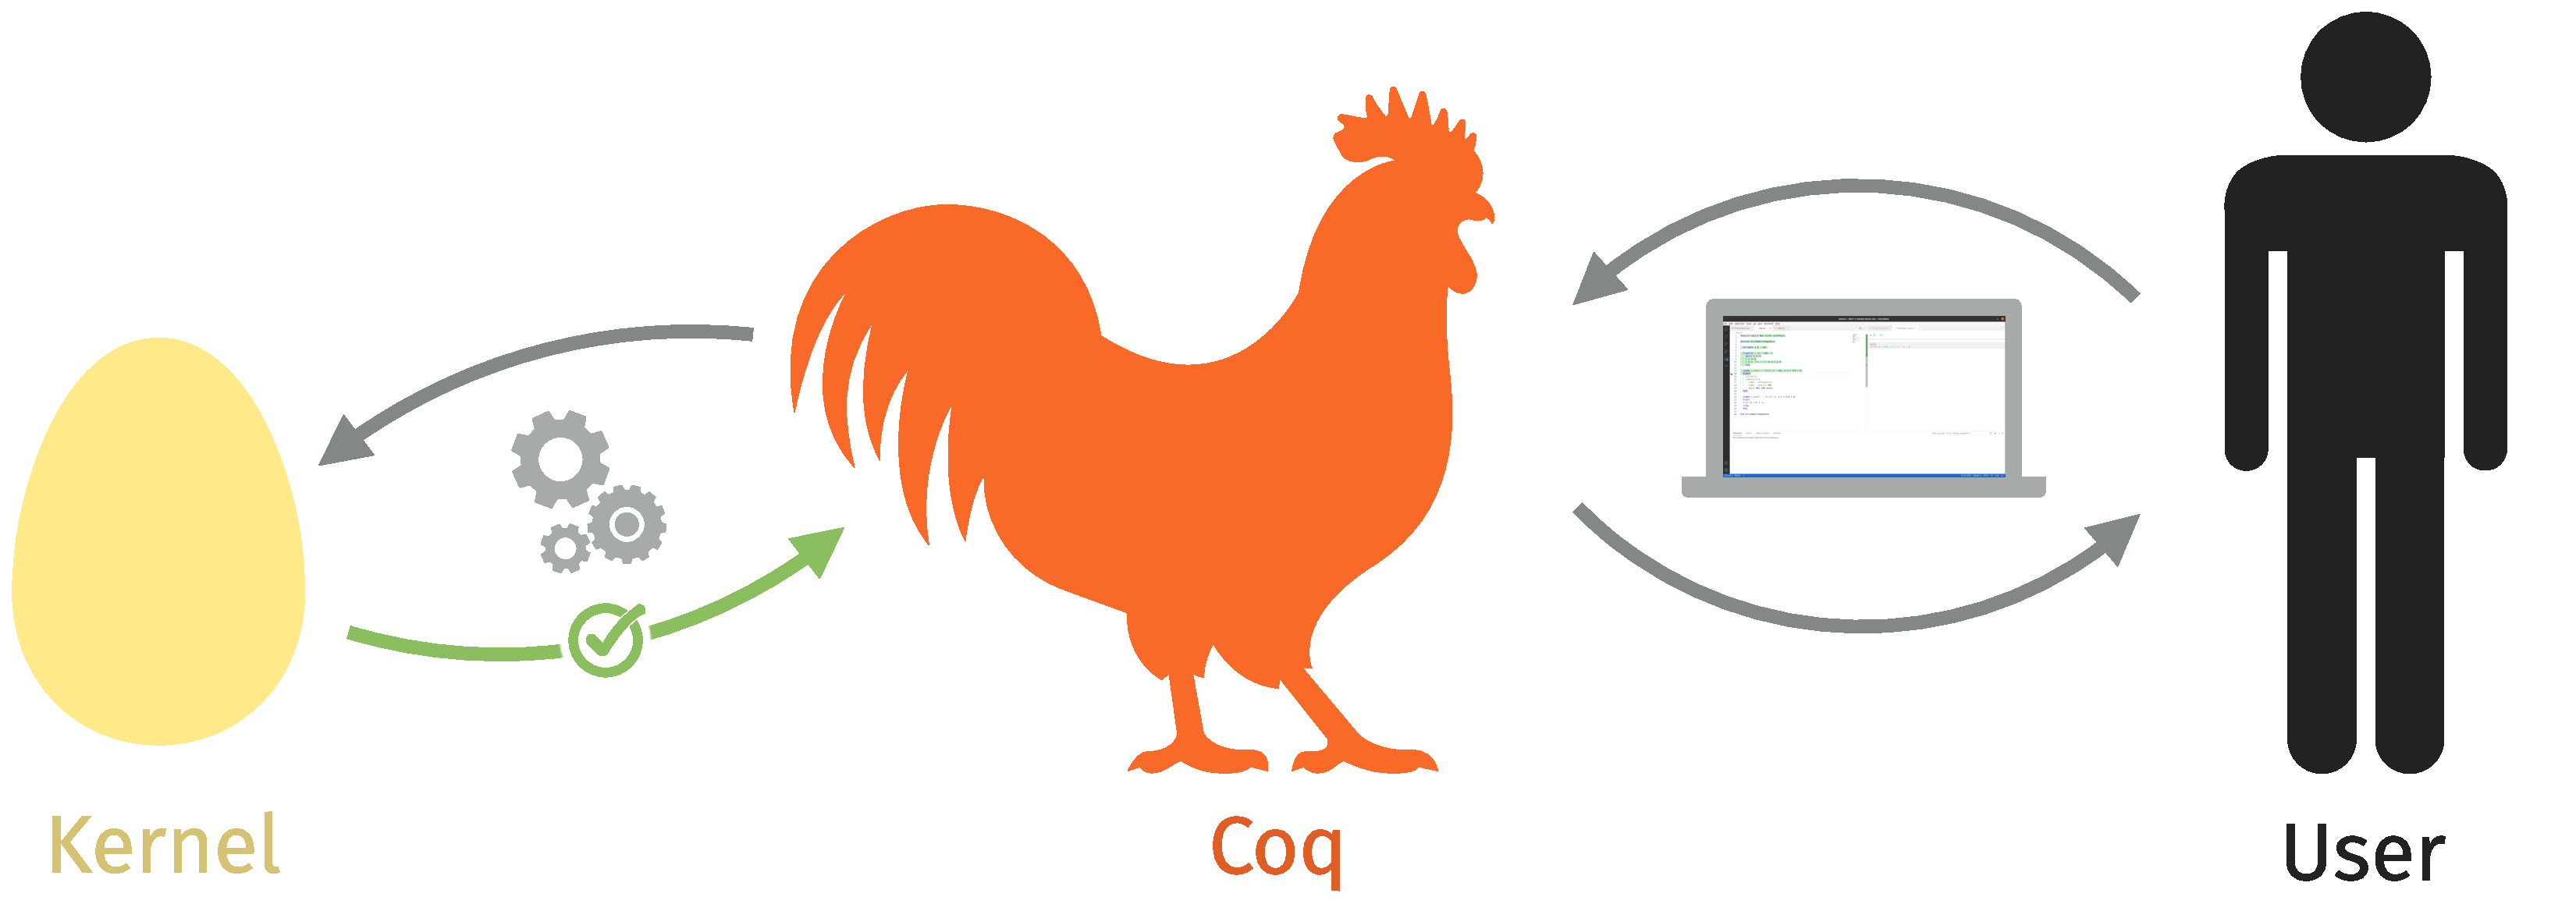
\includegraphics{./figures/coq-kernel-fr.pdf}

  \caption{Le fonctionnement schématique de Coq}
  \label{fig-coq}
\end{figure}

Coq est basé sur la \kl{correspondance de Curry-Howard} : les preuves sont vues comme des programmes dans un langage appelé \intro{Gallina},
et leur vérification est effectuée par un algorithme proche
de ceux utilisés pour les types des langages conventionnels.
Cependant, si dans les premières versions des années 80 \kl{Coq} ressemblait à un langage de programmation un peu étrange, ce n’est actuellement plus du tout le cas.
La raison, comme on l’a expliqué plus haut, est que \kl{Coq} est un \emph{assistant} à la preuve.
C’est pourquoi la majeure partie de \kl{Coq} dans ses versions actuelles a pour but d’aider l’utilisatrice à générer une preuve correcte sans avoir à l’écrire directement.
Ce fonctionnement est illustré en \cref{fig-coq} : l’utilisatrice échange interactivement avec \kl{Coq}, qui utilise cette interaction pour générer un terme de preuve. Celui-ci est ensuite envoyé à une partie bien spécifique du système, appelée \intro{noyau}.
C’est lui qui implémente l’algorithme de vérification de type, et s’assure ainsi de la correction des termes de preuve construits interactivement.
Le \kl{noyau} est donc l’élément crucial du système, car c’est lui – et lui seul – qui est responsable en dernier recours de la validation des preuves.


Cette architecture, qui isole clairement la partie critique du système
est appelée \intro{critère de de Bruijn}~\sidecite{Barendregt2001}, en 
hommage à l’un des pionniers des assistants à la preuve.
% Elle a permis de mener à bien des projets de grande ampleur, parmi lesquels CompCert~\sidecite{Kaestner2017} – un compilateur optimisant pour le langage C entièrement prouvé correct –, ou les preuves du théorème des quatre couleurs~\sidecite{Gonthier2007} et du théorème de l’ordre impair~\sidecite{Gonthier2013}, deux théorèmes importants et difficiles respectivement de la théorie des graphes et des groupes.
Cependant, si le reste de l’écosystème s’est beaucoup plus développé que le \kl{noyau} depuis les débuts, celui-ci a également évolué, en se complexifiant graduellement.
Et comme tout développement logiciel, il n’est pas à l’abri de bugs\sidenote{De l’ordre d'un bug détecté par an, une liste est maintenue à l’adresse suivante : \url{https://github.com/coq/coq/blob/master/dev/doc/critical-bugs}.}.
Ceux-ci sont en général difficilement exploitables par une utilisatrice de \kl{Coq}, encore plus sans s’en rendre compte.
Néanmoins, ils existent, et la tendance à la complexification du \kl{noyau} ne risque pas de s’arrêter de si tôt.

\subsection{MetaCoq, une formalisation par Coq, pour Coq}
\label{sec:intro-metacoq}


Si on veut garantir un niveau de fiabilité le plus élevé possible, il faut donc de nouvelles idées.
Le projet \intro{MetaCoq}, a pour but de répondre à cette problématique.
L’idée est simple : il s’agit d’utiliser \kl{Coq} lui-même pour certifier la correction de son \kl{noyau}.

Plus précisément, la première étape est de décrire à haut niveau le système de type sur lequel est basé le \kl{noyau}, puis de démontrer ses propriétés théoriques.
% , comme la confluence de la réduction, la préservation du typage par cette même réduction, etc.
Une fois ces propriétés établies, la deuxième étape consiste à programmer un algorithme de vérification de type ressemblant au maximum à celui du \kl{noyau}, directement en \kl{Gallina},\sidenote{
  En effet, grâce à la \kl{correspondance de Curry-Howard}, \kl{Gallina} est certes un langage pour décrire des preuves, mais aussi un véritable langage de programmation fonctionnel !}
tout en démontrant qu’il est bien correct\sidenote{
  Si l’algorithme prétend qu’un terme est bien typé, alors c’est bien le cas.}
et complet\sidenote{
  L’algorithme répond bien affirmativement sur tous les termes bien typés.}.
Enfin, une troisième étape extrait de ce programme \kl{Gallina} certifié
un programme efficace qui puisse être utilisé en lieu et place du \kl{noyau} actuel.
Cette extraction est elle-même complexe, car pour obtenir ce programme efficace il
faut effacer le contenu lié à la preuve de correction
pour ne garder que le contenu algorithmiquement intéressant.
C’est pourquoi là encore on prouve que l’extraction est correcte\sidenote{
  C'est-à-dire qu’elle préserve la sémantique des programmes.},
à nouveau en la programmant en \kl{Gallina}.

\subsection{Vérification et inférence}

Pour prouver la complétude de l’algorithme de typage, il est très utile de
passer par une spécification intermédiaire plus structurée que la description
théorique du système de type utilisée dans la première étape.
En particulier, il est important de séparer deux problèmes proches, mais
différents :
d'une part, la vérification, où on cherche à \emph{vérifier}
qu’un terme a bien un type
donné ; de l’autre, l’inférence, où on cherche à \emph{trouver}
un type pour un terme, s'il existe.
L’algorithme de typage du \kl{noyau} de \kl{Coq} est bidirectionnel,
c'est-à-dire qu’il alterne en permanence entre ces deux problèmes
lorsqu’il vérifie qu’un terme est bien typé.
% Par exemple, dans le cas d’une application $f~u$, il commence par inférer un type pour $f$, vérifie qu’il s’agit d’un type produit $\P x : A . B$ (une généralisation du type fonctionnel $A \to B$), puis vérifie que $u$ a le type $A$.
Décrire formellement cette structure bidirectionnelle plus proche de l’algorithme
permet de bien diviser les difficultés entre d’un côté
son équivalence avec la présentation
originale, et de l’autre la partie purement liée aux questions d’implémentation.

Dans le cadre spécifique des types dépendants, bien que présent depuis l’origine dans les algorithmes de vérification de type~\sidecite{Huet1989},
le typage bidirectionnel a été étonnamment peu étudié. En particulier, une preuve
de l’équivalence entre cette présentation et celle utilisée de manière standard
dans la littérature manquait !
Pourtant, cette approche présente également
des avantages théoriques : elle permet,
par sa structure plus contrainte que la présentation standars,
d’obtenir des propriétés difficiles à démontrer dans ce cadre standard.

\subsection{Un peu de flexibilité dans un monde désespérément statique}
\label{sec:intro-graduel}

Comme le cas de \kl{MetaCoq} l’illustre, \kl{Coq} peut être utilisé comme un véritable langage
de programmation. Mieux : son système de type, grâce à son extrême expressivité, 
permet d’exprimer des propriétés très complexes des programmes, et de vérifier
avant même d’exécuter les programmes que celles-ci sont bien respectées par le code.
Cependant, cette impossibilité d’écrire du code imparfait peut aussi se retourner contre l’utilisatrice, en complexifiant la phase de développement.
En effet, personne n’écrit du code parfait au premier essai. Les garanties très
fortes sur le code une fois finalisé compliquent donc 
fortement la phase de développement.
Une solution pour faciliter cette phase de développement
est de s’inspirer d’une proposition issue de la théorie des langages de
programmation : le \kl{typage graduel}. Ici encore, la \kl{correspondance de Curry-Howard}
est à l’œuvre, puisqu’on adapte des concepts venant du monde de la programmation
au cadre de la logique.

Il existe deux grandes approches de la vérification du type des programmes.
Dans l’approche statique\sidenote{Qui est celle sur laquelle est basée \kl{Coq}.},
les types sont vérifiés en amont de l’exécution, alors que dans l’approche dynamique le bon typage des opérations est vérifié à la volée lors de cette même exécution.
La discipline dynamique est plus flexible, parce qu’elle permet de vérifier exactement ce qui est nécessaire à la bonne exécution d’un programme.
À l’inverse, la rigidité du typage statique permet de détecter des erreurs plus tôt dans le développement, et impose des invariants utiles pour optimiser la compilation ou l’exécution.
Pourquoi choisir ? Le programme de recherche du \intro{typage graduel}~\sidecite{Siek2015} vise à dépasser ce dilemme, en intégrant dans un même langage disciplines statiques et dynamiques.
L’idée est d’avoir une première passe de vérification avant l’exécution, comme en typage statique, tout en laissant la possibilité de déférer des vérifications de type à l’exécution, comme en typage dynamique.
On a alors accès à tout un spectre de possibilités, d’une discipline totalement statique à une discipline totalement dynamique,
en pouvant choisir finement quelles parties d’un programme on veut vérifier à quel moment. En particulier, on peut faire évoluer la discipline au fur et à mesure d’un développement logiciel, pour bénéficier de la flexibilité du typage dynamique dans les phases précoces et des garanties du typage statique par la suite.

\section{Et cette thèse, alors ?}
\label{sec:cette-these}

Mon travail de doctorat lui-même
est centré principalement autour du typage bidirectionnel, sous
trois aspects, correspondant aux trois parties de cette thèse.

\subsection{Théorie du typage bidirectionnel}

La première partie (\nameref{part:bidir}) répare (une partie du) manque d'étude
théorique dans la littérature du typage bidirectionnel pour les types dépendant. Elle contient en particulier la
preuve de l’équivalence entre la présentation standard de la littérature et celle
bidirectionnelle.
Le \cref{chap:bidir-ccw} présente les idées générales qui guident ce travail
dans un cadre relativement simple, afin de faciliter leur exposition. 
Le \cref{chap:bidir-cic} montre comment étendre ces idées à un
cadre plus réaliste, proche de la théorie des types utilisée en pratique dans \kl{Coq}.
Enfin le \cref{chap:bidir-conv} traite du statut particulier de la
conversion\sidenote{Cette notion cruciale permet d’intégrer dans la
  théorie des types dépendants l’idée de calcul des programmes.}
et des liens du typage bidirectionnel avec certains travaux récents
à ce propos.

\subsection{Typage bidirectionnel dans MetaCoq}

La seconde partie de cette thèse (\nameref{part:metacoq})
concerne le projet \kl{MetaCoq}
et en particulier sur la formalisation, en \kl{Coq}, des idées présentées dans la
première partie. Le \cref{chap:metacoq-general} donne une présentation générale du
projet, tandis que le \cref{chap:kernel-correctness} se concentre spécifiquement
sur la preuve que le \kl{noyau} implémenté par \kl{MetaCoq} respecte sa spécification.

\subsection{Élaboration bidirectionnelle pour le typage graduel}

Enfin la troisième et dernière partie (\nameref{part:gradual})
présente mon travail
dans le domaine des \kl{types graduels}. Les types dépendants formant déjà des systèmes
complexes, l’adaptation de ceux-ci à l’approche graduelle est particulièrement
délicate. Un résumé des possibilités et problématiques associées est présentée
en \cref{chap:gradual-dependent}.
Un point intéressant est que la présentation habituelle
des types dépendants est inadaptée,
car elle est trop flexible. La structure additionnelle apportée
par le typage bidirectionnel est donc encore une fois cruciale.
De plus, celle-ci s’est avérée très agréable pour présenter
l’élaboration de termes depuis un langage source dans un langage cible, une
caractéristique importante des \kl[graduel]{langages graduels}.
L’utilisation d’une élaboration bidirectionnelle, et les propriétés qu’elle
permet d’obtenir, sont décrites en \cref{chap:bidir-gradual-elab}.

\subsection{Contributions personnelles}

Mon travail de doctorat a débuté avec l’étude des \kl{types dépendants} \kl{graduels}.
J’ai contribué avec Kenji Maillard, Nicolas Tabareau et Éric Tanter à
\sidetextcite{LennonBertrand2020}, où nous étudions une extension graduelle
pour le Calcul des Constructions Inductives. Mon travail technique s’est
majoritairement concentré sur le contenu correspondent au \cref{chap:bidir-gradual-elab}.
Le \cref{chap:gradual-dependent} est également tiré de cette publication.
Un second article, avec les mêmes auteurs et dans la continuité du précédent,
est actuellement en phase de relecture. Cependant il
ne fait pas appel directement au typage graduel, c’est pourquoi il n’en
sera pas question dans cette thèse.

Ce travail ayant montré la nécessité d’un système de types bidirectionnel
et le manque de résultats précis sur le sujet, je l’ai
étudié plus en détail, à la fois sur papier et par le biais d’une
formalisation se basant sur \kl{MetaCoq},
ce qui a donné lieu à une seconde publication~\sidecite{LennonBertrand2021},
et correspond aux \cref{chap:bidir-ccw,chap:bidir-cic}, et à une partie du
\cref{chap:kernel-correctness}.

J’ai ensuite travaillé à intégrer cette formalisation à
\kl{MetaCoq}, et à l’utiliser afin de montrer la complétude du \kl{noyau}
qui y est implémenté. Ceci correspond au reste du \cref{chap:kernel-correctness}.
Au-delà de cette contribution principale,
j’ai également participé à ce projet sur d’autres points plus mineurs.
Cette partie de mon travail de thèse n’a pas encore été publié, mais nous y
travaillons actuellement avec les autres contributeurs de \kl{MetaCoq}.

Enfin le \cref{chap:bidir-conv} correspond à un travail que j’ai entamé dans
le but d’étendre \kl{MetaCoq}, mais qui n’a pas encore atteint le stade de la
publication.

\selectlanguage{english}

\chapter{Introduction (English)}
\label{chap:intro-en}

\margintoc

This thesis belongs to the domain of \kl[dependent type]{type theory}, itself
at the crossroads between computer science and mathematical logics.
One of its goals is to give theoretical and practical foundations
for software tools helping humans in constructing and verifying proofs –
in the mathematical sense.
Such tools are called \kl{proof assistants}, and in this thesis one of them, on
which my work was mainly focused, is central: \kl{Coq}.

To replace this work in its larger context, this introduction begins with a very
short history of mathematical logics (\cref{sec:logic-history}), which exposes the
main questions of the field. Follows a presentation of the links between logics and
computer science, through \kl{proof assistants} (\cref{sec:proof-assistants}).
Next, \cref{sec:intro-coq-en} focuses more closely on the research questions I worked on.
Finally, \cref{sec:this-thesis} summarizes the contributions appearing in the rest of
this thesis.

\section{A very short history of logics}
\label{sec:logic-history}

\subsection{Syllogisms}

The main question that logics looks to answer is that of finding criteria in order to determine
if a reasoning is valid. In Western tradition, this challenge can be traced back to the
Antiquity, and particularly to Aristotle's \textit{Organon}.
The main contribution of this work is to introduce the notion of syllogism.
These are simple fragments of reasoning, which validity stems from the
fixed structure they follow, rather than a specific content.%
\sidenote{The most well-known is probably the \textit{Barbara} syllogism, and example
of which is: \emph{all humans are mortals; Socrates is human; so Socrates is mortal.}}
If complex reasoning is built from assembling such syllogisms, it must necessarily be valid as
a whole, since every assembled fragment is. There are here two important ideas.

The first is that reasoning can be valid or not, depending only on its structure,
independently of its content. Indeed, the whole focus of logics as a discipline from that
point on will concentrate on this structure which underlies reasoning.
It can be syllogisms, but many other systems. We will come across a certain number of them
in this thesis!

The second idea is that of a construction from elementary components.
Starting from a set of rules
one has identified as valid \textit{a priori}, we have a means to ensure the validity
of potentially very complex reasoning. In order to do so, it suffices to verify that these
can be decomposed into the base components.

At that time already, logics was conceived as a means towards communication.
The aim was of course to check one’s own reasoning, but also to be able to convey
it, by fixing a logical formal system%
\sidenote{Structural rules reasoning should obey, as those of syllogisms.}.
A person wanting their conclusion to be accepted by others only has to express their
reasoning in a perfectly precise way in the framework of such a formal system.

The main challenge of logics is thus to construct such a formal system, adapted to a specific
field of reasoning. In the case we are interested in, mathematical logics, this
enables us to give a precise meaning to what constitutes a valid mathematical proof.


\subsection{The beginning of mathematical logics: towards a formal foundation}[Towards a formal foundation]

Following Aristotle, mathematicians seized logics in order to build a formal system
able to serve as a rigorous foundation for mathematics.
Even though the links between logics and mathematics go back to Greek Antiquity,
important progress was made during the 19\textsuperscript{th} century, on two main aspects.

The first consisted in freeing mathematical logics from natural languages%
\sidenote{By opposition with the formal languages which appear in mathematics,
  computer science, etc.},
unsuited to a formal description of deduction, and to instead design a new form of language
specific that could serve as a basis for mathematical reasoning.
An important step here is \citeauthor{Begriffsschrift}'s
\citetitle{Begriffsschrift}~\sidecite{Begriffsschrift}, which, for the first time,
gives a formal language rich enough to express mathematics satisfyingly. Its
major addition is the notion of quantifier, essential to the mathematical vernacular,
which give a faithful way to account for universal%
\sidenote{For instance: “Every even integer is the sum of two prime numbers”.}
and existential%
\sidenote{For instance: “There exists an integer whose square is 2”.}
properties.

The second aimed at showing that mathematics as a whole could be reconstructed from a
few simple properties. An important step was the reduction of analysis to the properties
of real numbers, followed by constructions of those from arithmetic given almost
simultaneously in 1872 by \sidetextcite{Dedekind1872} and
\sidetextcite{Cantor1872}, among others.
Meanwhile, \sidetextcite{Peano1889} proposes an axiomatization of integers close to the
one still used today. Finally, Cantor again proposes set theory \sidecite{Cantor1883}
as a formalism expressive enough to describe all mathematical object as sets of elements.

\subsection{The foundational crisis of mathematics}[The foundational crisis]

Unfortunately, the system proposed in the \citetitle{Begriffsschrift} is inconsistent%
\sidenote{
  That is, it is possible to use it to prove falsity, and so it cannot serve as
  a satisfactory foundation for mathematics.
} !
This result by Russell%
\sidenote{
  Remarked by Russel in 1902, in a letter to Frege he made public
  in \textcite[Nachwort p.~253]{Frege1903}.}%
\margincite{Frege1903}
marks the opening of a crisis period.
Indeed, it cast doubt upon the systems that had started to establish
themselves as good candidates to serve as foundations – that of Frege, but
mainly those of Cantor, which were affected by the same difficulties.

A possible solution is suggested ten years later  by \citeauthor{Whitehead1913} in their
\citetitle{Whitehead1913} \sidecite{Whitehead1913}. This colossal piece of work
not only proposes a formal system avoiding the paradoxes leading to the inconsistency
of \citetitle{Begriffsschrift}. It also builds a significant amount
of mathematics in this system, including a construction of integers,
some arithmetic, and finally real numbers.

In parallel, in the continuity of Cantor’s work, \sidetextcite{Zermelo1908} and others
work towards giving a version of Cantor’s set theory that is consistent. This leads to what
is colloquially referred to as Zermelo-Fraenkel set theory – ZF, or ZFC when the
axiom of choice \sidecite{Zermelo1904} is added –, which also seems able to serve as a
solid foundation for mathematics.

\subsection{Incompleteness}

The search for a formal system adequate as a foundation for mathematics however hits a
second major difficulty: Gödel’s incompleteness theorem \sidecite{Goedel1931}. It asserts
that a formal system in which one can construct integers such as those of Peano – and so
\textit{a fortiori} any system rich enough to serve mathematician’s needs – cannot
prove its own consistency. Thus, no formal system can serve as a basis for mathematics
with a formal certitude as to its adequacy.
Indeed, as we cannot prove the consistency of the system in itself, it could very well
turn out to be inconsistent, ruining all the efforts put into its use – just like what
happened with Frege’s \citetitle{Begriffsschrift}.

A consequence of this theorem is that a system rich enough to found mathematics is
necessarily incomplete.%
\sidenote{
  This means that there exist independent statements, that is assertions which
  can neither be proven nor disproven – meaning that their negation is proven.
  The consistency of the system under consideration is one of many examples.
}
Thus, in what follows, I will never refer to truth in an absolute sense – which could
only be meaningful in a complete system where every statement is true or false –, but
only about provability \emph{relatively to a given system}.

\subsection{A satisfying situation ?}

Despite the difficulties put into light in the beginning of the 20\textsuperscript{th}
century, the research in mathematical logics came to a globally satisfying situation.
First, ZFC is a reasonable formal system on which mathematics can be founded. Moreover,
the mathematical community is globally convinced it would be \emph{theoretically} possible
to write down all mathematics using ZFC. This is enough for most of its members,
even if those who attempt to actually give it a try, in the vein of the
\citetitle{Whitehead1913}, are quite few.

In \emph{practice}, however, things are very different. The human development and
verification of formalized mathematics%
\sidenote{
  That is, effectively expressed in a fixed formal system.}
seems both impossible, and unnecessary.
On the one hand, it would demand a considerable effort, because such mathematics would
require an extremely high level of precision, both from the author of the formal proof
and from the reader. At the same time, this would not significantly reduce the risk of
errors. It would indeed be humanly very hard to check that some reasoning doubtlessly
follows the rules of the system: a tiny error can easily creep inside thousands of pages
of formal reasoning. Finally, describing mathematics in this way would drown the vital
mathematical intuitions, making communication sterile.

If we wish to make formal mathematics practicable, we thus need new tools.

\section{Computers enter the scene}
\label{sec:proof-assistants}

A new element however radically modifies the previous situation: the advent of computers.
Indeed, computer science provides new tools, making formalized mathematics both possible
and attracting.

\subsection{Proof assistants}

Computers excel where humans are weak: their speciality is to treat large volumes of
information in a very precise way, exactly the kind of needs brought up when manipulating
formalized mathematics. Therefore, already at the beginning of the 70s%
\sidenote{With systems like Automath \cite{DeBruijn1970}, or Mizar
  \cite{Rudnicki1992}.}%
\margincite{DeBruijn1970}%
\margincite{Rudnicki1992},
software tools, collectively called \intro{proof assistants}, had started to
appear. They are dedicated to writing and verifying formal proofs.
Through the formalization of proofs and the verification by computers that they
actually follow the rules of the underlying logical system, proof assistants open the
door to a level of trust much higher than that allowed by “informal” proofs.
Renown mathematicians, such as \sidetextcite{Voevodsky2010},
\sidecite[][Preface, p. xi]{Hales2012}, or \sidetextcite{Scholze2021} have indeed
turned to proof assistants, particularly in order to lift uncertainties regarding the
solidity of their own work.

But the term proof \emph{assistant} has not been chosen randomly : beyond simple verification,
proof assistant provide users with a large range of techniques to ease the conception of
formal proofs. These techniques usually enable users to write proofs at a rather
high level, and in an interactive manner%
\sidenote{In most modern proof assistants, the final proof is built as the result of
  an exchange between the programmer and the tool, rather than written as a single block.},
leaving it to the proof assistant to construct the formal proofs.
It can be simple facilities, such as the possibility to visualize the structure of proofs,
the tracking of hypotheses…

But computer science is much more powerful, it enables automatization of entire parts of
proof writing, for instance through the use of tactic languages \sidecite{Delahaye2000},
with which one can program proof generation.
In addition, the automatic construction of proofs is a research field by itself,
and the question of its integration intro proof assistants is an active topic
\sidecite{Boehme2010,Ekici2017}. Computer science has also proven its worth in the
setting of mathematical computations (computer algebra systems, numerical analysis),
and here again promising interactions with proof assistants are starting to arise
\sidecite{Lewis2022,Melquiond2012}.

Finally, if the use of software eases the writing of proofs, proof assistants conversely
open new possibilities for programming. They indeed offer a natural framework to describe in
the same place the source code of a program, its specification, and the formal proof that the
former fulfils the latter. This way, we can \emph{prove} that the program runs correctly,
without encountering any bugs.
This mathematical certainty is much more reliable than any test set!

\subsection{Logics, programming and type theory}

In order to work, proof assistants must be founded on a formal system, corresponding to
the “rules” of the mathematical “game” they are supposed to enforce.
Thus, they require a renewed study of mathematical logics, but with the practical aim of
building tools that are at the same time practical, powerful and easy to use.
There are multiple families of proof assistants, based on relatively different formal systems.
The one I am interested in in this thesis relies on the \kl{Curry-Howard correspondence}
and \kl[dependent type]{dependent type theory}. The proof assistant \kl{Coq},
which is at the heart of my work, belongs to this family.

If one compares a computer program with a text in a natural language,
\intro(en){types}
are a kind of equivalent of grammatical categories. However, contrarily to natural
languages, these types are conceived at the same time as the programming language, in order
to mirror properties of the objects it manipulates.
Their first use is to detect manifest errors. For instance, if a procedure
intended for an object of type “image” is applied to an object of type “character string”,
an error can be reported to the programmer.%
\sidenote{A well-known slogan due to \textcite{Milner1978} claims that
“Well-typed programs cannot go wrong.”}%
\margincite{Milner1978}
But types are very versatile, and their capacity to encode properties of the underlying
programs can be used for compilation, documentation, and many other things. In our
framework, for instance, types correspond to the validity of a logical reasoning.

\begin{marginfigure}

  % \begin{mathpar}
  %   \inferrule{ \Gamma, A \vdash B}{\Gamma \vdash A \Rightarrow B} \and
  %   \inferrule{\Gamma \vdash A \Rightarrow B \\ \Gamma \vdash A}{\Gamma \vdash B} \and
  %   \inferrule{\Gamma, x : A \vdash t : B}{\Gamma \vdash \lambda x : A . t : A \to B} \and
  %   \inferrule{\Gamma \vdash f : A \to B \\ \Gamma \vdash u : A}{\Gamma \vdash f~u : B}

  % \end{mathpar}

  % \caption{Règles d’inférence pour l’implication et de typage des fonctions}

  \begin{mathpar}
    \inferrule{A \\ B}{A \wedge B} \and
    \inferrule{A \wedge B}{A} \and
    \inferrule{A \wedge B}{B} \\
    \inferrule{a \ty A \\ b \ty B}{(a,b) \ty A \times B} \\
    \inferrule{p \ty A \times B}{p.1 \ty A} \and
    \inferrule{p \ty A \times B}{p.2 \ty B}
  \end{mathpar}
  
  \caption{Inference rules for conjunction and typing rules for pairs}
  \label{fig:curry-howard-example-en}
\end{marginfigure}

This idea is that of the \intro{Curry-Howard correspondence}. Rather than a precise theorem,
it is more of a very general concept, according to which two worlds closely resemble each
other: on the one hand, that of logics and proofs, on the other that of programs
and their types.

A short example says more than a long abstract talk, so let’s look at the correspondence
at work in \cref{fig:curry-howard-example-en}, in the form of inference/typing rules:
each bloc presents a rule, with above the bar the hypotheses, and below the conclusion.
The first three rules govern the logical conjuction “and”, written $\wedge$.
The first means that to deduce the proposition $A \wedge B$ (“$A$ and $B$”), it is enoguh
to deduce $A$ and $B$ taken individually.
Conversely, if we have as hypothesis $A \wedge B$, then we can deduce both $A$ (second rule),
and $B$ (third rule).
The last three rules govern typing%
\sidenote{Written using a colon.}
for the pair type $A \times B$. A pair $(a,b)$ built
from a first object $a$ of type $A$ and a second object $b$ of type $B$ has type $A \times B$.
Conversely, if $p$ is a pair of type $A \times B$, then we can retrieve its first component
$p.1$, which is of type $A$, and its second $p.2$, of type $B$.
If we erase the terms%
\sidenote{ In the context of type theory, we often talk about \emph{terms} instead of programs,
  but the two are synonyms.
}
of the bottom rules, we obtain \emph{exactly} the rules above!
Thus, the programming construct of pairs corresponds to the logical concept of conjunction.

This extends well beyond the specific case of conjunction, in a general correspondence
between, on one side, logical propositions and their proofs, and, on the other, types and programs.
We can see properties as types, and a proof of a given property as a program of the
corresponding type – or the other way around!
Beyond a simple analogy between formalisms of different origins, this correspondence
is a powerful tool to establish a dialogue between two worlds. In particular, it
relates two \textit{a priori} quite distant problems: checking that a proof
is valid, and checking that a term is well-typed. In both cases, it amounts to checking that
a construction – program on one side, proof on the other – respects a set of formal
rules guaranteeing it is well-formed.

The \kl{Curry-Howard correspondence} is therefore ideal to serve as a foundation for
\kl{proof assistants}, since it gives access, when studying formal logical systems,
to the rich literature on programming languages, in particular on the theory and
implementation of type systems. In this framework, the
\intro[dependent types]{dependent type systems} are a specific family of type systems,
whose main characteristic is the ability for types to depend on terms. The archetypical
example from the point of view of programming is the type $\Vect(A,n)$
of vectors of length $n$. These are lists that contain exactly $n$ elements of type $A$ – with
$n$ an integer.
This type depends on $n$, in the sense that its inhabitants differ depending on its value.
From the point of view of logics, this dependency corresponds to quantification: if we
wish to express a universal property “for all $x$, the property $P(x)$ holds”, then we need
the property $P$ to depend on $x$.
Thanks to this ability to express quantification, dependent types are rich and powerful enough
to serve as foundations for mathematics.

\section{Coq and its kernel}
\label{sec:intro-coq-en}

Let us focus a bit more on the proof assistant which we will consider mainly in this
thesis: \kl{Coq}.

\subsection[The kernel]{The kernel, cornerstone of the system}

\begin{figure}[h]

  \centering
  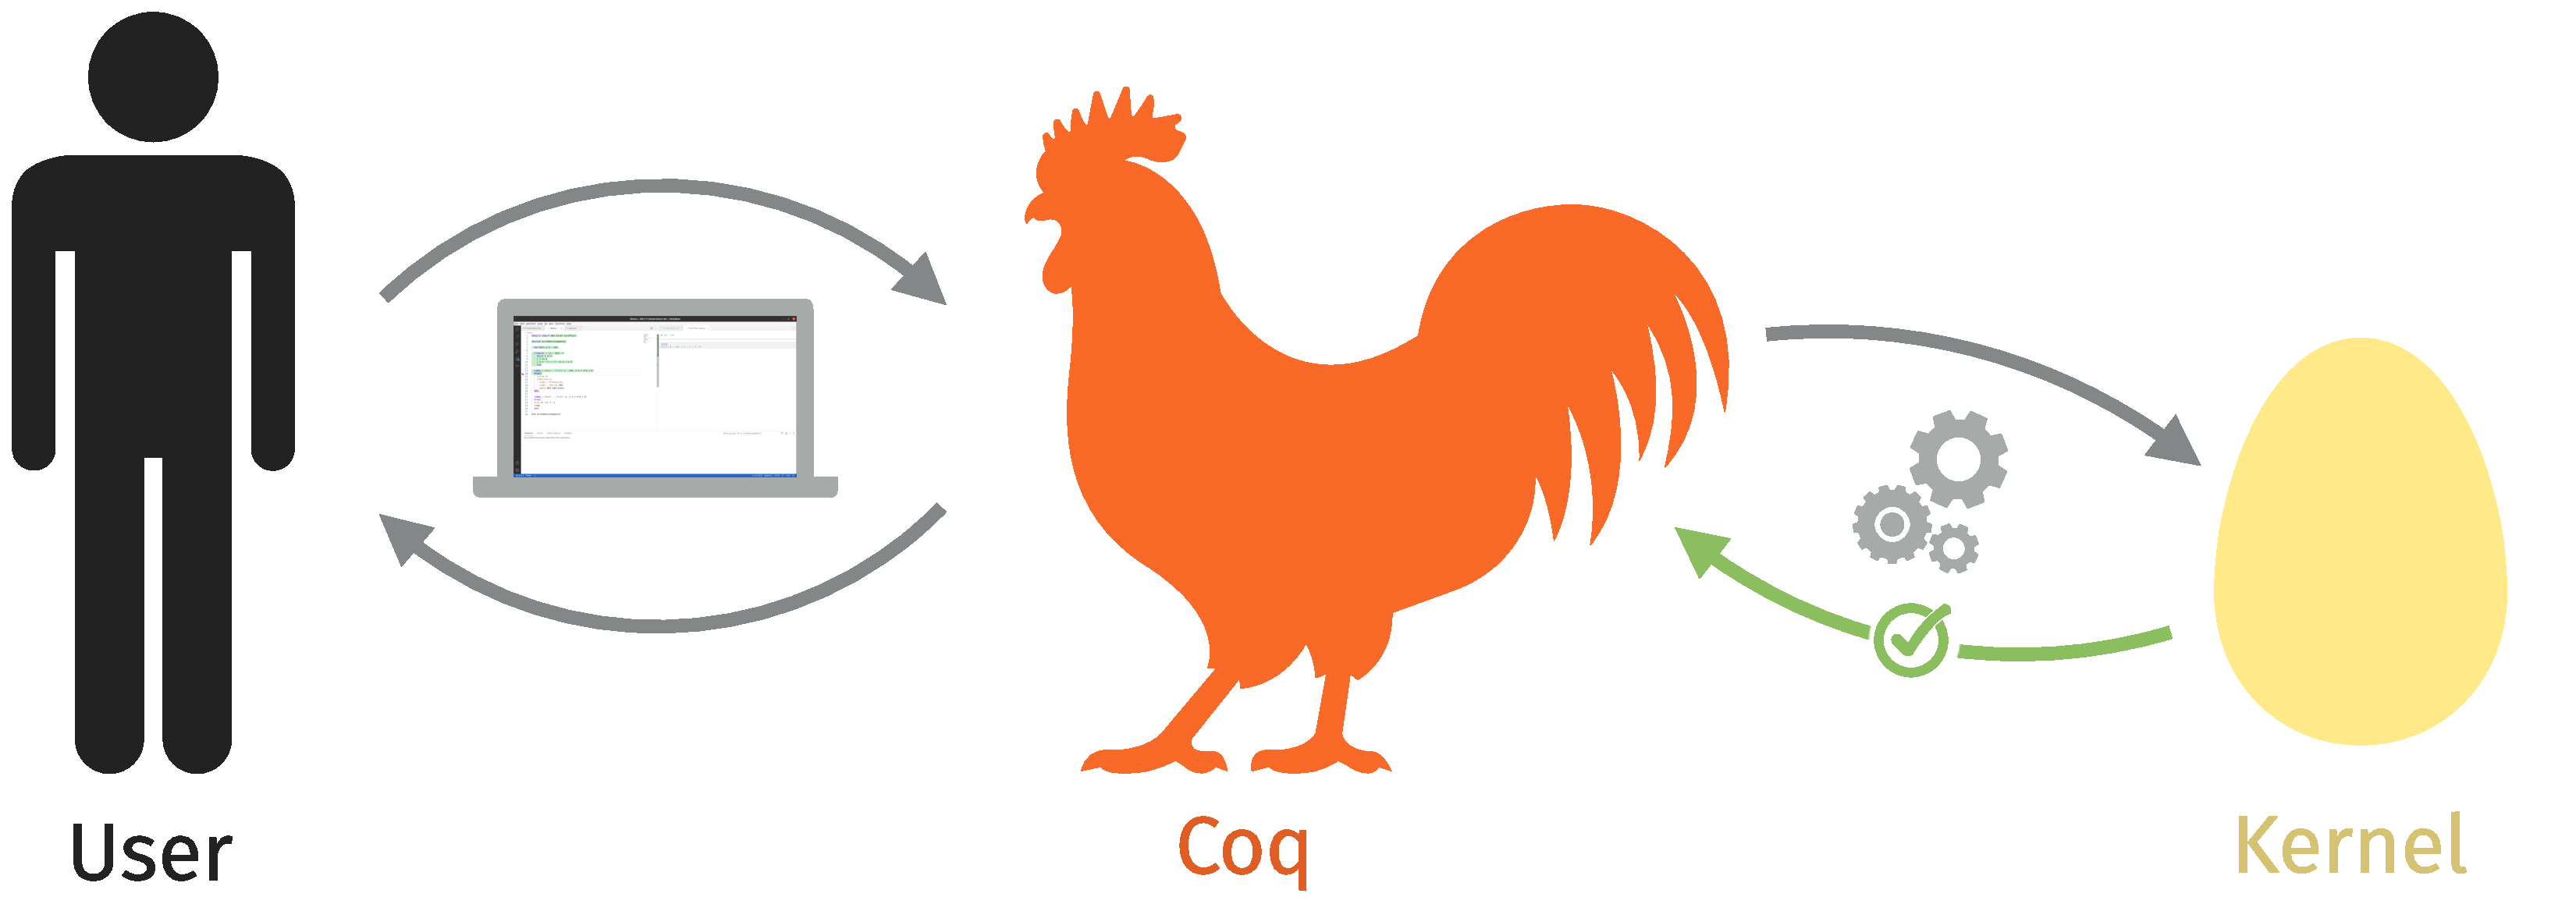
\includegraphics{./figures/coq-kernel-en.pdf}

  \caption{\kl{Coq}’s schematic architecture}
  \label{fig:coq-en}
\end{figure}

\kl{Coq} is based upon the \kl{Curry-Howard correspondence}: proofs are seen as programs,
in a language called \intro{Gallina}, and their verification is done using an algorithm
close to those used for types in conventional languages. However, if, in the first versions
from the 80s, \kl{Coq} looked like a somewhat esoteric programming language, it is
no longer the case at all. The reason is that the major part of the tool in its
current versions aims at helping the user in generating a correct proof. It is a true
\kl[proof assistant]{proof \emph{assistant}}!
The way \kl{Coq} works is illustrated in \cref{fig:coq-en} : the user interactively exchanges
with \kl{Coq}, which uses this interaction to generate a proof term. This proof term is then
sent to a very specific part of the tool, called the \intro{kernel}.
This is the part implementing the type-checking algorithm, and thus responsible for ensuring
that the proof terms built interactively are correct.
The \kl{kernel} is thus the crucial part of \kl{Coq}, because it is the one – and only –
ultimately responsible for proof-checking.

This architecture, which clearly isolates the critical part of the system, is called
\intro{De Bruijn criterion} \sidecite{Barendregt2001}, in tribute to one of the pioneer
of proof assistants.
If the rest of the ecosystem has grown much more than the \kl{kernel} since the beginning,
the latter has also evolved, becoming gradually more complex.
And, as any other software development, it is not safe from bugs%
\sidenote{ The magnitude is that of one critical bug found every year, a list is maintained
at the following address: \url{https://github.com/coq/coq/blob/master/dev/doc/critical-bugs}.}.
These are in general hard to exploit by a user, even more so without noticing.
But still, they exist, and since the \kl{kernel} tends to get more and more complex, they
are likely to continue appearing.

\subsection{\kl{MetaCoq}, a formalization in \kl{Coq}, for \kl{Coq}}[\kl{MetaCoq}]

If we wish to guarantee a trust level as high as possible in the \kl{kernel}, we must
resort to new ideas. That is what the \kl{MetaCoq} project is all about. The idea
is simple: using \kl{Coq} itself to certify the correctness of its \kl{kernel}.

More precisely, the first step is to describe formally the type system on which the \kl{kernel}
is based, and to show its theoretical properties.
Once these are established, the second step
% \sidenote{This is the one on which I mostly work, and on which we will come back in more
% length later on.}
consists in implementing a type-checking algorithm as close as possible to the one of the
\kl{kernel}, directly in \kl{Gallina}%
\sidenote{Indeed, thanks to the \kl{Curry-Howard correspondence}, \kl{Gallina} is of
course a proof language, but also a true programming language!}.
We show, while defining the algorithm, that it is indeed \reintro(bidir){correct}%
\sidenote{If the algorithm pretends that a term is well-typed, then it is the case.}
and \reintro(bidir){complete}%
\sidenote{The algorithm answers positively on all well-typed programs.}.
Finally, in a third step, we extract out of this certified \kl{Gallina} program another
more efficient program, by erasing the content related to the proof of correctness, in order
to keep only the algorithmically relevant one.
This extraction is a complex step, but crucial if we wish to replace the current \kl{kernel}
while keeping a reasonable efficiency. Therefore, we prove that said extraction
is correct%
\sidenote{Meaning that it preserves the semantics of programs.},
once again by programming it in \kl{Gallina}.

\subsection{Checking, inference and bidirectional typing}[Bidirectional typing]

During the second phase, in order to prove that the algorithm is complete, it is
very useful to go through an intermediate specification, which is more structured
than the theoretical one of the first phase.
In particular, it is important to separate two close, but very distinct, questions:
on the one side, type-checking, where we try and \emph{check} that a term indeed has a
given type;
on the other side, inference, where we try and \emph{find} a type for a term, if such a
type exists.
The typing algorithm of \kl{Coq}'s \kl{kernel} is \intro{bidirectional}, that is, it
alternates constantly between these two processes when it checks that a term is well-typed.
The closeness of the bidirectional structure to the algorithm allows for a
clear separation between, on the one side, its equivalence with the original formalization,
and on the other, the part purely dedicated to implementation questions.

In the specific case of dependent types, even if present in type-checking algorithms since
the origin – see \eg \sidecite{Huet1989} –, bidirectional typing has been relatively little
studied. However, beyond its strong relation to algorithms, this approach also presents
theoretical advantages: its more constrained structure makes it easier
to obtain properties that are difficult to obtain in the standard context.

\subsection{Gradual types: some flexibility in a desperately static world}
  [Gradual types]
\label{sec:intro-graduel-en}

There are two main approaches to program type-checking. In the static approach%
\sidenote{On which \kl{Coq} is based.},
types are verified prior to the execution, whereas, in the dynamic approach, the well-typedness
of the operations is verified on the fly during that same execution.
The dynamic discipline is more flexible, as it verifies exactly what is necessary
for the good execution of a program.
The strictness of static typing, conversely, allows for error detection earlier in the
development, and imposes invariants useful to optimize compilation or execution.
Instead of opting exclusively for one of the two approaches,
\reintro{gradual typing} \sidecite{Siek2015} aims at integrating
the static and dynamic disciplines in one and the
same language. This gives access to a whole spectrum of options, from a rigid completely static
discipline to a flexible dynamic one. It particularly allows for a fine-grained, local choice
of how each part of a program is type-checked.
One can thus evolve the discipline during software development, benefiting from
the flexibility of dynamic typing in early phases, and from the guarantees of static typing
later on.

As the case of \kl{MetaCoq} illustrates, \kl{Coq} can be used as a true programming language.
Even better: its type system can express very complex properties of programs, and thus
verify even before their execution that the code indeed enforces them.
Sadly, this impossibility to write imperfect code can turn against the user, by making the
early development phase more difficult. Indeed, nobody writes correct code on the first try,
and it would often be nice to temporarily lift the strong guarantees of typing to
facilitate experimentation. The idea would then be to take inspiration from gradual typing,
in order to pave the way for a more flexible logical or software development. Once again,
\kl{Curry-Howard correspondence} is at work, since we adapt concepts from the world of
programming languages to the logical one.

\section{And this thesis?}
\label{sec:this-thesis}

My doctoral work itself is centered around bidirectional typing, under three main aspects,
corresponding to the three parts of this thesis.
They are preceded by \cref{chap:tech-intro}, which introduces the main technical notions
used in what follows.

\subsection{Theory of bidirectional typing}

The first part (\nameref{part:bidir}) proposes to fill a part of the theoretical gap around
bidirectional typing for dependent types. More precisely, it contains a proof of equivalence
between the standard presentation of the literature, and a bidirectional one.
\Cref{chap:bidir-ccw} presents the general ideas that guide this work in a relatively
simple setting, in order to ease the exposition. \Cref{chap:bidir-pcuic} shows how to extend
them to a more realistic setting, close to the type theory implemented in \kl{Coq}.
Finally, \cref{chap:bidir-conv} focuses on the particular status of conversion%
\sidenote{This crucial notion allows the integration into dependent type theory of
the notion of computation of programs.},
and the links between recent work on this subject and bidirectional typing.

\subsection{Bidirectional typing in \kl{MetaCoq}}

The second part of the thesis (\nameref{part:metacoq}) focuses on the \kl{MetaCoq} project,
and especially the formalization, in \kl{Coq}, of the ideas presented in the first part.
\Cref{chap:metacoq-general} gives a general overview of the project, while
\cref{chap:kernel-correctness} concentrates more specifically on the proof that the
\kl{kernel} implemented in \kl{MetaCoq} fulfils its specification.

\subsection{Gradual dependent types}

Finally, the third and last part (\nameref{part:gradual}) presents my work in the area
of \kl{gradual types}. Since dependent types already form complex systems, their adaptation
to the gradual approach is particularly delicate. A summary of the possibilities and issues is
presented in \cref{chap:gradual-dependent}. An interesting point of emphasis is that the
usual presentation of dependent types turns out to be unsuited, as it is too flexible.
The additional structure provided by bidirectional typing is thus key. It also
appeared relevant to present the type-directed elaboration of terms from a source language
to a target one, an important characteristic shared by all\kl[gradual@typ]{gradual languages}.
The use of a bidirectional elaboration, and the properties it allows us to obtain, are described
in \cref{chap:bidir-gradual-elab}. Finally, \cref{chap:beyond-gcic} succinctly describes the
rest of the work I took part in regarding gradual types, but which is not directly
linked to bidirectional typing.

\subsection{Technical contributions}

My doctoral work started with the study of \kl(typ){gradual}
\kl(typ){dependent} types.
I contributed, together with Kenji Maillard, Nicolas Tabareau and Éric Tanter, to
\sidetextcite{LennonBertrand2022}, where we study a gradual extension to the
Calculus of Inductive Constructions. My main technical contribution corresponds
to \cref{chap:bidir-gradual-elab}. \Cref{chap:gradual-dependent} also comes from this
publication. A second article, together with the same authors and in the continuity of the
previous one, is currently under peer-reviewing. It is quickly summarized in
\cref{chap:beyond-gcic}, together with the second technical part of
\textcite{LennonBertrand2022}, whose main contributor is Kenji Maillard.

This work having shown the relevance of a bidirectional dependent type system and the relative
scarceness of results on the subject, I focused more closely on it, both on
paper and by means of a formalization based on \kl{MetaCoq}. This led to a second publication
\sidecite{LennonBertrand2021}, and corresponds to \cref{chap:bidir-ccw,chap:bidir-pcuic},
and parts of \cref{chap:kernel-correctness}.

I then turned to the integration of this formalization into \kl{MetaCoq}, and its use
in order to prove completeness of the \kl{kernel} it implements. This corresponds to the
rest of \cref{chap:kernel-correctness}. I also took part in the project on more minor points.
This part of my thesis work has not been published yet, but the other contributors to
\kl{MetaCoq} and I are currently working on it.

Finally, \cref{chap:bidir-conv} corresponds to a project I initiated in order to extend
\kl{MetaCoq}, but which did not reach the stage of publication yet.

\chapter{The Calculus of Inductive Constructions}
\label{chap:tech-intro}

Most of this thesis revolves around \kl[dependent type]{dependent type systems}.
Since these are
quite complex, there is a high number of points where one can introduce slight variations
when giving a precise definition of a system to study it.
Some of these variations are unimportant, but some introduce large differences in the
resulting systems. Thus, in this chapter we go over in details over
the definition of what we refer to as the
\kl{Calculus of Inductive Constructions} (or simply \kl{CIC}), in the rest of this
thesis, and which serves as the basis for variations, theoretical study and extensions.
While doing so, I try to give an idea of the trade-offs involved, and of the reasons
behind the choices made. Quite a few of those choices vary during the thesis,
and this is by design: there is no single better choice, 
something that I try to make as clear as possible.

For the impatient specialists, let me say now that with \kl{CIC}, I
mean an intentional type theory, with Curry-style abstractions,
a predicative hierarchy of universes \textit{à la Russel}\sidenote{
  And only those: by default I do \emph{not} include an impredicative sort of propositions, a feature that is sometimes associated to the name \kl{CIC}.},
and any amount of required inductive types, presented by recursors – 
the ones appearing most often in what comes next being the empty and
unit types, booleans, natural numbers, dependent sums, lists, vectors and the equality.
Conversion is by default the reflexive, symmetric, transitive and congruent
closure of β-reduction, and
so in particular it is untyped. For the others, let me now detail what I mean by this.

\section{Terms, typing and derivations}

Throughout this chapter, type systems are defined by means of a relation
$\Gamma \vdash t : T$, which reads "in the context $\Gamma$, term $t$ has type $T$".
From the logical point of view, this judgement means that $\Gamma$
contains the hypothesis available to deduce the
result $T$ by means of the proof $t$. On the programming side, it means that
$t$ is a well-formed program,
which uses the variables listed in $\Gamma$ together with their types,
and has type $T$.
Thus, $\Gamma$ is a list of declarations of the form $x : A$. We write $\emptycon$ for the
empty context, and $\Gamma, x : A$ for the context $\Gamma$ extended with the new variable $x : A$, and $(x : A) \in \Gamma$ to denote that the declaration $x : A$ appears at some
point in the context $\Gamma$.

\begin{marginfigure}
  \begin{mathpar}
  \inferdef{Var}{(x : A) \in \Gamma \\ \vdash \Gamma}{\Gamma \vdash x : A}
  \label{rule:cic-var}
  \end{mathpar}
\end{marginfigure}

This typing relation itself is defined by means of inference rules,
such as \ruleref{rule:cic-var} opposite. The way to read this rule is that the judgement
underneath the line follows from the one above,
\ie from $(x : A) \in \Gamma$
and $\vdash \Gamma$ – a judgement that will soon be defined asserting that the context
$\Gamma$ is well-formed – we can deduce $\Gamma \vdash x : A$.
When objects appear in the hypothesis but not the conclusion, they are implicitely
universally quantified.
Once a set of such inference rules is fixed,
typing is defined as the least relation closed by those
rules. Equivalently, a judgement such as $\Gamma \vdash t : T$
holds as soon as we can build a tree whose nodes are instances of the inference rules,
and whose root is the judgement in question. A general setting
to make this kind of definitions precise can be found in \sidetextcite{Bauer2020},
in our case we restrict to this level of detail until \arefpart{metacoq}.

As we have already introduced variables, a word on those as well. Variables are difficult
to account for precisely, because of issues like shadowing – a conflict between two variables
with the same name – or $\alpha$-equivalence – the identification between two terms
only differing on variable names. There are multiple techniques to solve these issues
– see the many solutions to the POPLMark Challenge~\sidecite{Aydemir2005} –, 
but again, we treat these issues in an informal way until \arefpart{metacoq}, assuming
there is no shadowing whatsoever and identifying $\alpha$-equivalent terms when needed.

A final important building block that we use in all our type theories is substitution,
that we write $\subs{t}{x}{u}$. This replaces every occurrence of $x$ in $t$ by the term
$u$. Once again, we treat this operation informally, assuming it never creates
shadowing – what is sometimes called "capture-avoiding" substitution.

\section{Functional core: \kl{CCω}}
\label{sec:tech-ccw}

\subsection{Functions and applications}

Let us now turn to the core of CIC, namely the
\intro{Calculus of Constructions} (\kl{CCω}). Through the \kl{Curry-Howard correspondence},
it is both a typed form of λ-calculus – \ie a kind of purely functional
programming language – and a minimal form
of logic – only containing universal quantification and implication.

\begin{marginfigure}
  \ContinuedFloat*
  \begin{mathpar}
    \inferrule{\Gamma, x : A \vdash t : T}{\Gamma \vdash \l x : A .\ t : A \to T}
    \and
    \inferrule{\Gamma \vdash f : A \to T \\ \Gamma \vdash u : A }{ \Gamma \vdash t\ u : T}
  \end{mathpar}
  \caption{Typing for non-dependent functions}
  \label{fig:cic-nondep-fun}
\end{marginfigure}

Functions, also called λ-abstraction are written $\l x : A .\ t$. This corresponds
to the mathematical notation $x \mapsto t$: the body $t$ of the function,
is a term that might contain the variable $x$,
and the constructor λ abstracts over that variable to build a function.
Conversely, function application is written simply using juxtaposition, as in $t\ u$.
The type of functions is written $\to$, as in ordinary mathematics.
You can see those at work in \cref{fig:cic-nondep-fun}: an abstraction build a term of arrow
type, and application needs its function to be of arrow type, whose domain must correspond to
that of the argument for it to be well-typed.
Logically, those rules correspond to that of implication: if from a hypothesis $A$ one can
deduce $T$, then $A \to T$ holds – reading $\to$ as implication; conversely if $A \to T$
and $A$ both hold, then $T$ does as well.

\begin{marginfigure}
  \ContinuedFloat
  \begin{mathpar}
    \inferdef{Abs}{\Gamma, x : A \vdash t : T}{\Gamma \vdash \l x : A .\ t : \P x : A.\ T}
    \label{rule:cic-abs}
    \and
    \inferdef{App}{\Gamma \vdash f : \P x : A.\ T \\ \Gamma \vdash u : A }{ \Gamma \vdash f\ u : \subs{T}{x}{u}}
    \label{rule:cic-app}
  \end{mathpar}
  \caption{Typing for dependent functions}
  \label{fig:cic-dep-fun}
\end{marginfigure}
These arrow types, however, are not as expressive as one would wish for.
Remember that we are in the realms of dependent types, so not only $t$ might mention $x$,
but also $T$. For instance, $T$ might be something like "$x$ is even". In such a case,
we need to record that dependency, which is the point of $\P$-types – or product types –,
shown in \cref{fig:cic-dep-fun}.
Seen as function types, they record the fact that the codomain
might vary depending on the argument. This is reflected in the typing rule for application:
since the codomain $T$ might depend on $x$, the type of the application $f\ u$ is $T$
\emph{specialized at the argument $u$}, using substitution.
Seen on the logical side, product types correspond to universal quantification
$\operatorname{\forall} x : A.\ T(x)$.
Indeed, if one can show that $T(x)$ holds for an unspecified $x$,
then it must hold for all $x : A$ – this is \ruleref{rule:cic-abs}.
Conversely, if $T$ holds for all $x : A$, then one can deduce $T(u)$ for any specific
$u : A$ – this is \ruleref{rule:cic-app}.
Now the rules for arrow types in \cref{fig:cic-nondep-fun} are just a special case
of those for product types, in the case where the codomain $T$ does not depend
on the variable $x$, and we use this convention throughout the thesis:
$A \to T$ is a shortcut for $\P x : A.\ T$ when $T$ does not mention $x$.

One last thing to note about our functions is that they record the type of their
domain – what is called \intro{Church-style}
abstraction~\sidecite[][Section~3]{Barendregt1992}. There is an alternative – 
the \intro{Curry-style} abstractions –, that
does not do so, simply using $\l x.\ t$ for functions. At this point in the
presentation, this does not make much difference,
but it is crucial as soon as one looks at the bidirectional structure. 
Indeed, that annotation is required if one wants to infer types for functions,
rather than barely checking them.
The \kl{Curry-style}
option is definitely sensible, see for instance \sidetextcite[][p.~19]{Norell2007}
– which describes the implementation of the very successful proof assistant
\kl{Agda}, which uses the \kl{Curry-style} approach –,
\sidetextcite[][Section~4.1]{Gratzer2019} or \sidetextcite{McBride2022}.
In the end, this is really a design choice between being able to infer a type for any term,
or requiring annotations that in a lot of cases are useless, and in this
thesis we stick with the approach used in \kl{Coq}, and annotate our abstractions.

\subsection{Universes}

To be able to express things like induction principles or polymorphic functions, it is
extremely useful to be able to use functions and products quantifying over types.
This is what the universe $\uni$ are for. It is the type… of a type.
This means that the frontier between types and terms is not syntactic any more.
Instead, types are simply terms of type $\uni$.
Despite this, we still use upper case letters for terms which we want to think of as types.
Such a universe is called \textit{à la} Russell~\sidecite{Palmgren1998}, by contrast with
universes \textit{à la} Tarski, which regain the distinction between types and terms at
the cost of a somewhat heavier treatment of types.
The presentation \textit{à la} Tarski
is mostly useful when building models. Since this is not the subject at hand in this thesis,
we keep the simpler of the two presentations.

\begin{marginfigure}
  \ContinuedFloat
  \begin{mathpar}
    \inferdef{Univ}
    {\vdash \Gamma}
    {\Gamma \vdash \uni[i] : \uni[\unext{i}]}
    \label{rule:cic-univ}
  \end{mathpar}
  \caption{Typing for universes}
  \label{fig:cic-univ}
\end{marginfigure}

There is however, an important caveat.
Since the disappointments of Frege and the paradox exhibited
by Russell in his system, logicians know that considering a set of all sets is a great
source of inconsistencies. Type theory is not devoid of this issue:
Girard~\sidecite[][Annex~A]{Girard1972}
shows how having a type with itself as type is inconsistent.
This inconsistency directly applies to the first dependent type system proposed by
Martin-Löf~\sidecite{MartinLoef1972}, which had a single universe $\uni$ and a rule $\uni : \uni$.
A common solution to this
is to stratify universes into an infinite hierarchy, which gives us \ruleref{rule:cic-univ}:
note the \intro{universe levels} $i$ and $\unext{i}$.

\begin{marginfigure}
  \ContinuedFloat
  \begin{mathpar}
    \inferdef{Prod}
    {\Gamma \vdash A : \uni[i] \\ \Gamma, x : A \vdash B : \uni[j]}
    {\Gamma \vdash \P x : A.\ B : \uni[\umax{i}{j}]}
    \label{rule:cic-prod}
  \end{mathpar}
  \caption{Typing for product types}
  \label{fig:cic-prod}
\end{marginfigure}

\begin{marginfigure}
  \ContinuedFloat
  \begin{mathpar}
    \inferdef{EmptyCon}
    { }{\vdash \cdot}
    \label{rule:cic-empty-con} \and
    \inferdef{ConsCon}
    {\vdash \Gamma \\ \Gamma \vdash A : \uni}{\vdash \Gamma, x : A}
    \label{rule:cic-cons-con}
  \end{mathpar}
  \caption{Context well-formedness}
  \label{fig:cic-con}
\end{marginfigure}

Using those universes, \ruleref{rule:cic-prod} gives the typing rule for the product constructor. We can also use these universes to give a definition of the $\vdash \Gamma$
judgement, asserting that a context is well-formed, in \cref{fig:cic-con}.
It simply means that all its types
are indeed types. Note that in \ruleref{rule:cic-cons-con}, we did not give an index for the
universe, we do so to mean the existence of some unconstrained level $i$.

One last important point regarding universes is the kind of levels used. The simplest solution
is to rely on natural number (of the meta-theory), with the $\unextsymb$
and $\umaxsymb$ operations interpreted by the usual ones.
This is however not strictly necessary: we need levels
to form an order so as to ensure we avoid inconsistency, and operations $\unextsymb$ and
$\umaxsymb$, but levels could very well be something different from natural numbers.
In particular, the natural number approach fixes at which level a particular construction
is done, which is usually much more rigid than what one would wish for.
A more flexible approach, introduced under the name \intro{typical ambiguity} by
\sidetextcite{Harper1991},
uses level expressions based on level variables, rather than integers.
This way, one can collect the constraints between levels required for a
term to type-check in a consistent system, without artificially enforcing a
rigid interpretation of levels by fixing them to a precise integer once and for all.
To simplify the presentation, our "standard" \kl{CCω}/\kl{CIC} nonetheless uses integers,
but we switch to level expressions when needed.

\section{50 Shades of Conversion}
\label{sec:tech-conversion}

\begin{marginfigure}
  \ContinuedFloat
  \begin{mathpar}
  \inferdef{Conv}
    {\Gamma \vdash t : T \\ \Gamma \vdash T \conv T' : \uni}
    {\Gamma \vdash t : T'}
  \label{rule:cic-conv}
  \end{mathpar}
  \caption{Conversion rule}
\end{marginfigure}

There is one big missing part in the picture so far. Remember we are working with
dependent types, and that those can contain terms, which in turn can be arbitrary programs.
If you recall for instance the vector type we used in the introduction (and that we are
about to introduce formally), what happens if a function expects an argument of type
$\Vect A\,3$, but it is given an argument of type $\Vect A\,(2+1)$, for instance the output
of a concatenation function? Surely we must have a way to relate both, since after all
the small program $2+1$ ought to compute to $3$! This is exactly what \intro{conversion} is
for: in dependent type theory, there is a way to change a type to one that
is related to it by this relation – this is \ruleref{rule:cic-conv}, which wraps up our typing
rules for \kl{CCω}, collected in \cref{fig:ccw-typing}.
As usual, there are two ways to look at this relation. From the point of view of programs,
it allows to incorporate the computational aspect of those, directly inside the type system.
From the point of view of logics, this corresponds to things being the same "by definition"
rather than due to some reasoning
– which is why conversion is also called definitional, or judgmental equality. In our vector
example, for instance, the two types are the same by virtue of the definition of addition.

\begin{figure*}[h]
  \LastFloat

  \begin{mathpar}
    %
    \jform{\vdash \Gamma}
    \inferdef{EmptyCon}
      { }{\vdash \cdot}
    \and
    \inferdef{ConsCon}
      {\vdash \Gamma \\ \Gamma \vdash A : \uni}{\vdash \Gamma, x : A}
    \\\\
    \jform{\Gamma \vdash t : T}
    \inferdef{Var}{(x : A) \in \Gamma \\ \vdash \Gamma}{\Gamma \vdash x : A}
    \and
    \inferdef{Univ}
      {\vdash \Gamma}
      {\Gamma \vdash \uni[i] : \uni[\unext{i}]}
    \and
    \inferdef{Prod}
      {\Gamma \vdash A : \uni[i] \\ \Gamma, x : A \vdash B : \uni[j]}
      {\Gamma \vdash \P x : A.\ B : \uni[\umax{i}{j}]}
    \and
    \inferdef{Abs}{\Gamma, x : A \vdash t : T}{\Gamma \vdash \l x : A .\ t : \P x : A.\ T}
    \and
    \inferdef{App}
      {\Gamma \vdash f : \P x : A.\ T \\ \Gamma \vdash u : A }
      {\Gamma \vdash f\ u : \subs{T}{x}{u}}
    \and
  \inferdef{Conv}
    {\Gamma \vdash t : T \\ \Gamma \vdash T \conv T' : \uni}
    {\Gamma \vdash t : T'}
  \end{mathpar}

  \caption{Collected typing rules for \kl{CCω}}
  \label{fig:ccw-typing}
\end{figure*}

Conversion is a very complex beast, arguably the most subtle part of dependent types.
Consequently, there are very different ways to present it, which in turn serve different
needs.
For this reason, we took care to setup the typing rules of
\cref{fig:ccw-typing} so that \emph{nothing} has to
be changed in those when one definition of conversion or another is taken. The only
difference is in how the relation $\Gamma \vdash T \conv T' : \uni$ is defined.
This way, we can treat it as a black box when talking about typing,
making the design modular.

A first divide is between \intro[typed conversion]{typed} and
\intro[untyped conversion]{untyped} conversion.
On one side, conversion is intrinsically typed, terms are only convertible
\emph{at a given type}. On the other, conversion is a relation between raw terms,
that does not presuppose any form of typing. \Cref{fig:typed-untyped-conv} gives an
example of the "same" rule – the computation rule for functions – in both systems.
As we can see, the content of the two rules is the same, it equates $(\l x : A.\ t)\ u$
and $\subs{t}{x}{u}$, only the side-conditions differ wildly.
Typed conversion goes back to
\sidetextcite{MartinLoef1972}, and is a recurring feature in its many descendants.
Untyped conversion relates strongly to (untyped) λ-calculus – Barendregt
for instance uses the name "conversion" for the equational theory of untyped λ-calculus
in his reference work on the subject~\sidecite{Barendregt1985} –, via
the Pure Type Systems (PTS)~\sidecite{Barendregt1991} literature.
In this thesis, we mainly consider untyped conversion, as \kl{Coq}’s meta-theory
has been mostly studied in that tradition.
But the relation between both in the context of
bidirectional typing is the main subject of \cref{chap:bidir-conv}.

\begin{figure}[h]
  \begin{mathpar}
    \inferrule
      {\Gamma, x : A \vdash t : B \\ \Gamma \vdash u : A}
      {\Gamma \vdash (\l x : A.\ t)\ u \tdconv \subs{t}{x}{u} : \subs{B}{x}{u}}
    \and
    \inferrule{ }{(\l x : A.\ t)\ u \udconv \subs{t}{x}{u}}
  \end{mathpar}
  \caption{Example: typed and untyped β rule for conversion}
  \label{fig:typed-untyped-conv}
\end{figure}

A second axis is about how close the conversion relation is to an implementation.
For instance, conversion should be an equivalence relation,
but there are two approaches to that. The first – and standard – one
is to simply \emph{define} conversion as an equivalence relation, by adding rules 
for \eg transitivity, as the one of \cref{fig:trans-conv}.
\begin{marginfigure}
  \begin{mathpar}
    \inferrule
      {t \udconv t' \\ t' \udconv t''}
      {t \udconv t''}
  \end{mathpar}
  \caption{Example: transitivity rule for conversion}
  \label{fig:trans-conv}
\end{marginfigure}
This ensures that conversion has the right properties, but means it does not directly correspond
to an algorithm: the transitivity rule cannot be directly implemented, since its middle
term is not recorded in any place.
The λ-calculus theorists have known this issue for a long time, and they
have a solution: characterizing conversion by means of a \kl{reduction} relation $\red$, which
corresponds to the idea of program evaluation – see \sidetextcite{Barendregt1985} for
instance. If this reduction has good
properties\sidenote{The main one being confluence.}, then
two terms are be convertible exactly when they reduce to the same third term.
This much more operational characterization is closer to what can be implemented.
Turning things around, one can define conversion through reduction,
and only show \emph{afterwards}
that it has the good properties of the first approach – typically, that it is transitive.
Conversion of the first kind we call \intro{declarative conversion}, while for the second
we talk about \intro{algorithmic conversion}.

In the rest of this section we give two presentations of \kl{untyped conversion}.
A \kl{declarative} one, which we use to define \kl{CCω}, as is the standard.
And an \kl{algorithmic} one, anticipating \arefpart{metacoq} where it is needed
to show decidability of type-checking, and
\arefpart{gradual} where we extend it into a relation that is by design not transitive, so
that basing it on declarative conversion would be nonsensical.

\subsection{Untyped declarative conversion}

\begin{marginfigure}
  \ContinuedFloat*
  \begin{mathpar}
    \inferdef{UConv}{\Gamma \vdash T' : \uni \\ T \udconv T'}{\Gamma \vdash T \conv T' : \uni}
    \label{rule:cic-conv-unty}
  \end{mathpar}
  \caption{Typing constraint on untyped conversion}
\end{marginfigure}

To start our presentation of \kl{untyped conversion},
let us first go back to \ruleref{rule:cic-conv}.
Even if we wish to describe conversion as
an untyped relation, we still enforce a typing constraint in \ruleref{rule:cic-conv},
in order to ensure that, whenever $\Gamma \vdash t : T$ is derivable,
$\Gamma \vdash T : \uni$ is as well.
This is exactly the content of \ruleref{rule:cic-conv-unty}, which combines conversion
with a check that the target type is indeed a well-formed type.

\begin{figure}[h]
  \ContinuedFloat
  \begin{mathpar}
    \inferdef{ConvRefl}{ }{t \udconv t}
    \label{rule:cic-uconv-refl} \and
    \inferdef{ConvSym}{t \udconv t'}{t' \udconv t}
    \label{rule:cic-uconv-sym} \and
    \inferdef{ConvTrans}
      {t \udconv t' \\ t' \udconv t''}
      {t \udconv t''}
    \label{rule:cic-uconv-trans}
  \end{mathpar}
  \caption{Equivalence rules}
  \label{fig:cic-uconv-equiv}
\end{figure}

Regarding conversion itself, the first set of rules asserts
that conversion forms an equivalence relation: it
is reflexive (\ruleref{rule:cic-uconv-refl}), symmetric (\ruleref{rule:cic-uconv-sym}),
and transitive (\ruleref{rule:cic-uconv-trans}).

A second set of rules, collected in \cref{fig:cic-uconv-cong},
asserts that conversion is a congruence, meaning that it is compatible
with all term formers. As for the previous three, these correspond to properties we expect
from the conversion relation, that we simply declare to be true. Note that we include only
congruence rules for term formers with sub-terms – we \eg omit $\uni$. This is because
those are special cases of \ruleref{rule:cic-uconv-refl}. Conversely, we could omit 
reflexivity altogether and only have congruence rules, which can be seen as a generalized
form of reflexivity.

\begin{figure}[h]
  \ContinuedFloat
  \begin{mathpar}
    \inferrule
    % \inferdef{ProdConv}
      {A \udconv A' \\ B \udconv B'}
      {\P x : A.\ B \udconv \P x : A'.\ B'}
    % \label{rule:cic-uconv-prod}
    \and
    \inferrule
    % \inferdef {AbsConv}
      {A \udconv A' \\ t \udconv t'}
      {\l x : A .\ t \udconv \l x : A'.\ t'}
    % \label{rule:cic-uconv-abs}
    \and
    % \inferdef{AppConv}
    \inferrule
      {f \udconv f' \\ u \udconv u' }
      {f\ u \udconv f'\ u'}
    % \label{rule:cic-uconv-app}
  \end{mathpar}
  \caption{Congruence rules}
  \label{fig:cic-uconv-cong}
\end{figure}

\begin{marginfigure}
  \ContinuedFloat
  \begin{mathpar}
    \inferdef{βConv}{ }{(\l x : A.\ t)\ u \udconv \subs{t}{x}{u}}
    \label{rule:cic-uconv-beta}
  \end{mathpar}
  \caption{Computation rule for functions}
\end{marginfigure}
Finally \ruleref{rule:cic-uconv-beta}, is the crucial one:
it corresponds to the computational behaviour
of functions, replacing the variable of an applied λ-abstraction by its argument by
means of substitution.

\subsection{Reduction}

Before we can describe \kl{algorithmic conversion}, we first need
to give a look at \intro{reduction}. Reduction is in some way an operational variant of
conversion. The main difference is that it is oriented, in the direction which would
correspond to program evaluation. It itself decomposes into three components.

\begin{marginfigure}
  \ContinuedFloat*
  \begin{mathpar}
    \inferdef{βRed}{ }{(\l x : A.\ t)\ u \tred \subs{t}{x}{u}}
    \label{rule:beta-red}
  \end{mathpar}
  \caption{Top-level reduction}
\end{marginfigure}

The first is \intro{top-level
reduction} $\tred$, which corresponds purely to computation, without any congruent closure.
In \kl{CCω} there is only the single \ruleref{rule:beta-red}.

The second component is the congruent closure of top-level reduction,
\intro{one-step reduction} $\ored$, which allows triggering top-level reduction exactly once,
but at any position in a term. Its definition is given in \cref{fig:ccw-ored}.
Note that while we talk about congruent closure both for
\kl{conversion} and \kl{one-step reduction}, we mean it differently: in the
case of conversion, we demand the relation to hold in all sub-terms,
while for one-step reduction it is allowed in exactly one position.

\begin{figure}[ht]
  \ContinuedFloat
  \begin{mathpar}
    \inferrule
    % \inferdef{TopRed}
      {t \tred t'}
      {t \ored t'}
    % \label{rule:top-red}
    \and
    \inferrule
    % \inferdef{ProdRedDom}
      {A \ored A'}
      {\P x : A.\ B \ored \P x : A'.\ B}
    % \label{rule:red-prod-dom}
    \and
    \inferrule
    % \inferdef{ProdRedCod}
      {B \ored B'}
      {\P x : A.\ B \ored \P x : A.\ B'}
    % \label{rule:red-prod-cod}
    \and
    \inferrule
    % \inferdef{AbsRedDom}
      {A \ored A'}
      {\l x : A .\ t \ored \l x : A'.\ t}
    % \label{rule:red-abs-dom}
    \and
    \inferrule
    % \inferdef{AbsRedBod}
      {t \ored t'}
      {\l x : A .\ t \ored \l x : A.\ t'}
    % \label{rule:red-abs-bod}
    \and
    \inferrule
    % \inferdef{AppRedFun}
      {f \ored f'}
      {f\ u \ored f'\ u}
    % \label{rule:red-app-fun}
    \and
    \inferrule
    % \inferdef{AppRedArg}
      {u \ored u'}
      {f\ u \ored f\ u'}
    % \label{rule:red-app-arg}
  \end{mathpar}
  \caption{One-step reduction}
  \label{fig:ccw-ored}
\end{figure}

Finally, we obtain \kl{reduction} as the reflexive
transitive closure of one-step reduction, see \cref{fig:red}.

\begin{figure}[h]
  \begin{mathpar}
    \inferrule
    % \inferdef{TopRed}
      {t \tred t'}
      {t \ored t'} \and
    % \label{rule:top-red}
    \inferrule{ }{t \fred t}
    \and
    \inferrule
      {t \ored t' \\ t' \fred t''}
      {t \fred t''}
  \end{mathpar}
  \caption{Reduction}
  \label{fig:red}
\end{figure}

Now, the reason we separate these three layers is that reduction as just defined is
somewhat too unrestricted, in particular it is non-deterministic.
In a lot of places, what we care about is exposing the head
constructor of a term, and there is a deterministic strategy we can impose to do so, called
\intro{weak-head reduction} $\hred$. It amounts to restricting the places in the term where
\kl{top-level reduction} can be used, by removing some congruence rules. More precisely,
λ-abstractions, product types and universes are not reduced, as they already are canonical
forms of their types. Variables are not reduced either, since they simply cannot be. Thus,
the only reduction that is allowed is in the function position of an application, with the
hope to get an abstraction there that can be further reduced at top-level. In the end,
we get \cref{fig:wh-red}. When we want to contrast this weak-head reduction with the
previously defined one $\red$, we call the latter \kl{full reduction}.
\begin{figure}[h]
  \begin{mathpar}
    \inferrule
    % \inferdef{TopRed}
      {t \tred t'}
      {t \hored t'}
    % \label{rule:top-red}
    \and
    \inferrule
      {f \hored f'}
      {f\ u \hored f'\ u}
    \and
    \inferrule{ }{t \hred t}
    \label{rule:red-refl} \and
    \inferrule
      {t \hored t' \\ t' \hred t''}
      {t \hred t''}
    \label{rule:red-trans}
  \end{mathpar}
  \caption{Weak-head redution}
  \label{fig:wh-red}
\end{figure}



\subsection{Algorithmic conversion}

\section{Adding Inductive Types: \kl{CIC}}

\subsection{Datatypes}

\subsection{Indexed inductive types}

\section{Beyond \kl{CIC}: \kl{PCUIC}}

\subsection{Cumulativity}

\subsection{The sort of propositions}

\subsection{Local and global definitions}

\subsection{Enhancing inductive types}

\subsection{Co-inductive types and records}

\pagelayout{wide} % No margins
\addpart{Bidirectional typing for dependent types}
\label{part:bidir}
\pagelayout{margin} % Restore margins


When presenting a typing derivation the way we did in \cref{chap:tech-intro}, there is
an important piece of information missing.
In logical programming, this is called the \kl{mode} of the inference rules,
\ie which objects are considered as inputs and which as outputs in the search
for a derivation.
This information, however, is crucial when one tries to build a type-checker:
some rules might seem fine when writing them down on paper, but trying to give them a
sensible mode fails, indicating they are not suited for an implementation.
In the case of the typing judgement $\Gamma \vdash t \ty T$,
usually both the term $t$ under inspection and the context $\Gamma$ are inputs –
although some depart from this, see \sidetextcite{Jim1996}.
The mode of the type $T$, however, is much less clear: should it be inferred based upon
$\Gamma$ and $t$, or do we merely want to check whether $t$ conforms to a given $T$?
Both are sensible approaches, and in fact typing algorithms for complex type systems usually 
alternate between them during the inspection of a single term/program.
The bidirectional approach makes this difference between modes explicit,
by decomposing \intro{undirected typing}%
\sidenote{We call anything related to the $\Gamma \vdash t \ty T$ judgement undirected,
by contrast with the bidirectional typing.}
$\Gamma \vdash t \ty T$ into two separate judgements $\Gamma \vdash t \inferty T$
(\kl{inference}) and $\Gamma \vdash t \checkty T$ (\kl{checking})%
\sidenote{We use the $\inferty$ and $\checkty$ symbols rather than the more usual
$\Rightarrow$ and $\Leftarrow$ to avoid confusion with implication and with the
\kl{Coq} notation for functions.},
that differ only by modes of the type. It is an output in inference, but an output in checking.
Following this decomposition, pionereed by \sidetextcite{Pierce2000}, gives rise to type
systems that are more structured, directly amenable to implementations,
and leads to algorithms which are often of good quality.%
\sidenote{\citeauthor{Pierce2000} for instance stress good error reporting as an important 
attribute of their approach.}

Although this seems appealing, and despite advocacy by \eg
\sidetextcite{McBride2018,McBride2019} to explicitly adopt this approach during
the design of type systems on paper rather than in their implementations only,
most of the theoretical work on dependent typing to this day remains undirected.
Bidirectionality appears mostly
in articles concentrating on the description of typing algorithms – for instance
\sidetextcite{Huet1989}, \sidetextcite{Coquand1996}, or \sidetextcite{Norell2007}…
However, since these primarily insist on the algorithmic aspect, they do not consider the
bidirectional structure for itself. Moreover, in the case of
\textcite{Coquand1996} and \textcite{Norell2007}, they concentrate on bidirectional typing
as a way to remedy for the lack of annotations on their \kl{Curry-style} λ-abstractions.
This is sensible when looking for lightness of the input syntax, but poses an inherent completeness problem: a term such as $(\l x . x)~0$ is not typeable in those systems.%
\sidenote{They are actually only able to give types to normal forms.}
In the context of \kl{Church-style} abstraction, the closest there is to a description of
bidirectional typing for \kl{CIC} is probably that by the
\kl{Mattia} team \sidecite{Asperti2012},
who however again concentrate on the challenges posed by the
elaboration and unification algorithms.
They also do not consider the problem of completeness with respect to a given undirected system, as it would fail in their setting due to the undecidability of higher order unification.

In this part we therefore wish to fill this gap in the literature,
by describing a bidirectional type system that is complete with respect to the (undirected)
\kl{Calculus of Inductive Constructions}, as presented in \cref{chap:tech-intro}.
By completeness, we mean that any term that is typeable in the undirected system should also
infer a type in the bidirectional one.
This feature is very desirable when implementing kernels for proof assistants,
whose algorithms should correspond to their undirected specification,
never missing any typeable term – even those not in normal forms.

The bidirectional system we present naturally forms an intermediate
step between actual algorithms and undirected type systems, something we exploit
in \arefpart{metacoq}.
But the interest of having a bidirectional type system equivalent
to the undirected one is not limited to the relation to algorithms.
Indeed, the structure of a bidirectional derivation is more constrained than that of
an undirected one, especially restraining the uses of computation.
This finer structure can make proofs easier,
while the equivalence ensures that they can be transported to the undirected world.
We show this by providing straightforward proofs of \kl{uniqueness of types}
up to cumulativity, and of \kl{strengthening}.

% The bidirectional structure also provides a better base for new type systems. This was actually the starting point for this investigation: in \cite{LennonBertrand2020}, we quickly describe a bidirectional variant of CIC, as the usual undirected CIC is unfit for the gradual extension we envision due to the too high flexibility of a free-standing conversion rule. This is the system we wish to thoroughly describe and investigate here.
 
% This step has proven useful in an ongoing completeness proof of MetaCoq's \cite{Sozeau2020a} type-checking algorithm\footnote{A completeness bug in that algorithm – also present in the Coq kernel – has already been found, see \cref{sec:to-pcuic} for details.}: rather than proving the algorithm complete directly, the idea is to prove it equivalent to the bidirectional type system, separating the implementation problems from the ones regarding the bidirectional structure.

This part is separated into three chapters.
As we did in \cref{chap:tech-intro}, we start by exposing the main ideas in the
simpler setting of \kl{CCω} in \cref{chap:bidir-ccw}.
With those set clear, we go on with their adaptation to \kl{PCUIC}, and the subtle
issues that arose in that context, in \cref{chap:bidir-pcuic}.
Finally, \cref{chap:bidir-conv} describes early investigations into giving a
bidirectional treatment not only of typing, but also of conversion.

% This equivalence has been formalised on top of MetaCoq \cite{Sozeau2020}\footnote{A version frozen as described in this article is available in the following git branch: \url{https://github.com/MevenBertrand/metacoq/tree/itp-artefact}.}
% We next turn back to less technical considerations, as we believe that the bidirectional structure is of general theoretical interest. \Cref{sec:beyond} thus describes the value of basing type systems on the bidirectional system directly rather than on the equivalent undirected one. Finally \cref{sec:related} investigates related work, and in particular tries and identify the implicit presence of constrained inference in various earlier articles, showing how making it explicit clarifies those.
\chapter{Warmup: CCω}
\label{chap:bidir-ccw}

\section{Turning \kl{CCω} Bidirectional}
\label{sec:bidir-ccw}

\section{Properties of the Bidirectional System}
\label{sec:bidir-prop}

\begin{itemize}
  \item Correctness
  \item Completeness
  \item Reduction strategies and uniqueness
  \item Strengthening
\end{itemize}
\chapter{Bidirectional \kl(tit){PCUIC}}
\label{chap:bidir-pcuic}

\margintoc

As we have seen in \cref{sec:tech-pcuic}, there is much more to the real \kl{Coq} than
\kl{CCω}.
The ideas exposed in the previous chapter nevertheless
scale very well to these extensions.
There are two areas, though, where some care needs to be taken.
The first is cumulativity, which in particular forces us to reconsider the statement
of the completeness and uniqueness properties, see \cref{sec:bidir-pcuic-cumulativity}.
But the main one is the introduction of inductive types. In particular, there is a subtle
interplay with cumulativity in the treatment of pattern-matching.
Working on the formalized proof of completeness in \kl{MetaCoq} led to the discovery of
an incompleteness bug in the kernel of \kl{Coq} linked to this.
In \cref{sec:bidir-pcuic-inductives} we show how the bidirectional setting adapts to
inductive types, and try and give an intuition of the origin of the completeness issue.

We do not give precise proofs in this chapter,
instead relying on the formalization in \kl{MetaCoq} as described in \arefpart{metacoq}.

  % The first area of difference are the universes. While on paper those are simply integer, to handle typical ambiguity and polymorphic (co)-inductive types, PCUIC uses algebraic universes, containing level variables, algebraic $\vee$ and $+1$ operators, and a special level for the sort Prop. Moreover, those universes are cumulative, that is they behave as if smaller universes were included in larger ones. The precise handling of the algebraic universes is abstracted away in MetaCoq, and quite similar in the directed and undirected systems, so it did not prove too difficult to handle. Cumulativity, however, introduces some not-so-small differences with the previous presentation, so we spend some time on it in \cref{sec:pcuic-cumul}.

  % The second is the addition of new base type and term constructors. We describe the treatment of inductive types in \cref{sec:pcuic-indu}. Co-inductive types and records behave very similarly to inductive types at the level of typing, so we do not dwell on them. The difference lies mainly at the level of reduction/conversion, but as our type system treats those as black boxes the differences have a negligible impact.
  
  
\section{Cumulativity}
\label{sec:bidir-pcuic-cumulativity}

\begin{marginfigure}
  \begin{mathpar}
    \inferdef{CheckCum}
    {\inferty{\Gamma}{t}{T} \\ T \cum T'}{\checkty{\Gamma}{t}{T'}}
    \label{rule:bd-check-cum}
  \end{mathpar}    
\end{marginfigure}
The introduction of the more liberal cumulativity rules in the undirected system
of course calls for an update to the computation rules.
The change to \ruleref{rule:bd-check} is direct: simply replace conversion with cumulativity,
as done in \ruleref{rule:bd-check-cum} opposite.
As for the constrained inference rules, they do not even need any modification.
Intuitively, this is because there is no reason to degrade a type to a larger one,
unless it is forced by a given target type in the checking judgment.

The statement of completeness also needs to account for cumulativity,
and becomes the following:

\begin{theorem}[Completeness, with cumulativity]
  \label{thm:comp-cumul}
  If $\Gamma \vdash t \ty T$, then $\inferty{\Gamma}{t}{T'}$ is derivable
  for some $T'$ such that $T' \cum T$.
\end{theorem}

This also means that in the setting of \kl{PCUIC},
\kl{uniqueness of types} up to \kl{conversion} is not true any more.
For instance, we both have $\Gamma \vdash \uni[0] \ty \uni[1]$ and $\Gamma \vdash \uni[0] \ty \uni[2]$, but $\uni[1]$ and $\uni[2]$ are not convertible. In that context, however,
the type $\uni[1]$ still has a special property: it is minimal amongst all types, what
we call a \kl{principal type}.

\begin{definition}[Principal type]
  The type $T$ is a \intro{principal type} for term $t$ – in a context $\Gamma$ –
  if $\Gamma \vdash t \ty T$ and for any $T'$ such that $\Gamma \vdash t \ty T'$,
  we have $T \cum T'$.
\end{definition}

The existence of such a principal type is the same as \kl{uniqueness of types} 
up to cumulativity. Moreover, even in the cumulative setting, \cref{thm:unique-inf}
stays true – intuitively, because it only relies on properties of reduction, but not of
conversion. Thus, following the same proof as that of \cref{thm:unique-undir},
we obtain the following:

\begin{theorem}[Inferred types are principal]
  \label{thm:princ-types}
  If $\Gamma$ is well-formed and $\inferty{\Gamma}{t}{T}$,
  then $T$ is a \kl{principal type} for $t$ in $\Gamma$.
\end{theorem}
  
\begin{proof}
  If $\Gamma \vdash t \ty T'$, then by completeness there exists some $T''$ such that
  $\inferty{\Gamma}{t}{T''}$, and moreover $T'' \cum T'$.
  But by \cref{thm:unique-inf}, $T \conv T'' \cum T'$ and thus $T \cum T'$, and $T$ is thus indeed a principal type for $t$ in $\Gamma$.
\end{proof}

The existence of \kl{principal types} is not so easy to prove directly, as it more or less
amounts to showing correctness and completeness of the bidirectional system at once.
Nevertheless, it is useful, because it in particular means that any well-typed term $t$
has an unambiguous smallest universe, which can be obtained as the \kl{principal
type} of its \kl{principal type}. This means that there is a good separation between irrelevant 
propositions – those terms whose smallest universe is $\Prop$ – and relevant terms
– those whose smallest universe is some $\uni[i]$ –, and that this stays true even in
presence of cumulativity, and even if $\Prop \cum \uni[i]$. If this were not the case,
the erasure of propositional content – which is one of the important use cases of $\Prop$ –
would not make sense.

\section{Inductive Types}
\label{sec:bidir-pcuic-inductives}

\subsection{An example: the pair type}

\begin{figure}
    
  \begin{mathpar}
    \inferdef{PairTy}{
      \pinferty{\uni}{\Gamma}{A}{\uni[i]} \\ 
      \pinferty{\uni}{\Gamma, x : A}{B}{\uni[j]}}
      {\inferty{\Gamma}{\Sb x : A .\ B}{\uni[\umax{i}{j}]}}
      \label{rule:pair-type-bd} \and
    \inferdef{Pair}{
      \pinferty{\uni}{\Gamma}{A}{\uni[i]} \\
      \pinferty{\uni}{\Gamma, x : A}{B}{\uni[j]} \\
      \checkty{\Gamma}{t}{A} \\
      \checkty{\Gamma}{u}{\subs{B}{x}{t}}}
      {\inferty{\Gamma}{\pair[A][x.B]{t}{u}}{\Sb x : A .\ B}}
      \label{rule:pair-bd} \and
    \inferdef{PairInd}{
      \pinferty{\Sb}{\Gamma}{s}{\Sb x : A .\ B} \\
      \pinferty{\uni}{\Gamma, z : \Sb x : A .\ B}{P}{\uni} \\
      \checkty{\Gamma, y_1 : A, y_2 : \subs{B}{x}{y_1}}{b}
        {\subs{P}{z}{\pair[A][x.B]{y_1}{y_2}}}}
      {\inferty{\Gamma}{\ind{\Sb}{s}{z.P}{y_1.y_2.b}}{\subs{P}{z}{s}}}
      \label{rule:pair-ind-bd} \and
        
    \inferdef{PairInf}{
      \inferty{\Gamma}{t}{T} \\ T \red \Sb x : A .\ B}
      {\pinferty{\Sb}{\Gamma}{t}{\Sb x : A .\ B}}
      \label{rule:sig-inf} 
  \end{mathpar}

  \caption{Bidirectional pair type}
  \label{fig:bidir-pair}
\end{figure}

To set ideas straight, let us look at how we can adapt the dependent pair type of
\cref{fig:sig} to the bidirectional setting: see \cref{fig:bidir-pair}.
To obtain these rules, first notice that all rules of \cref{fig:sig}
must become inference rules if we want the resulting system to be complete.
The question therefore is once again to choose modes for the premises.
Rules \nameref{rule:pair-type-bd} and \nameref{rule:sig-inf} are
very similar to the rule for Π-types, there is not much surprise there.

\ruleref{rule:pair-bd} shows why we insisted in the undirected system
on recording the types $A$ and $B$ in the pair. Indeed, they are needed to
know which type to infer for the pair. Without the annotation, one could infer a
type $A$ for $t$ and a type $B'$ for $u$, but there are potentially many incomparable types $B$ that would be correct for the whole pair, depending on which instances of $t$ in $B'$ are abstracted to $x$. This impossibility to invert a substitution is a general source of need
for annotations, which is not specific to pair types!

Finally, \ruleref{rule:pair-ind-bd} is the most complex.
In usual presentations of \kl{recursors}, the predicate appears first, then the branches,
and finally the scrutinee. But this is not possible here, as the parameters of the inductive
type are needed to construct the context in which the predicate is typed.
Instead, those parameters can be inferred from the scrutinee.
Thus, a type for the scrutinee is first obtained using a new constrained inference judgment,
forcing the inferred type to be a Σ-type, but leaving its parameters free.
Next, these parameters can be used to construct the context to type the predicate.
And finally, once the predicate is known to be well-formed,
it can be used to type-check the branch.

This same approach can be readily extended to the other inductive types of
\cref{sec:tech-cic}, with recursion or indices posing no specific problems.
%, see \cref{fig:bidir-indu-other}.

\subsection{Polymorphic Inductive Types}

The account of general inductive types in \kl{PCUIC} is slightly different from
the one we just gave. The reason for this is that giving a general account of rules
which infer type levels like our \ruleref{rule:pair-type-bd} is not easy.
Indeed, the parameters of an inductive type can
be of a type much more complex than simply $\uni$, and in that general setting deciding which
type variable can be inferred is a non-trivial problem.
Instead, the polymorphic inductive types as implemented in \kl{Coq} store explicit universe
levels on inductive types and constructors. The  pair type of \cref{fig:bidir-pair},
for instance, would contain explicit universe levels $i,j$, so that both $A$ and $B$
would be checked rather than having their level inferred.
The rule for the type constructor in that context is given opposite.
\begin{marginfigure}
  \inferrule{
    \checkty{\Gamma}{A}{\uni[i]} \\ 
    \checkty{\Gamma, x : A}{B}{\uni[j]}}
    {\inferty{\Gamma}{\Sb\ulev{i,j} x : A .\ B}{\uni[\umax{i}{j}]}}
\end{marginfigure}
This makes the treatment of complex inductive types possible by using checking uniformly –
rather than relying on constrained inference to infer universe levels –
at the cost of possibly needless annotations, as here with Σ-types.
This is mostly invisible for the end user hough, as she does very seldom write universe
levels thanks to \kl{typical ambiguity} anyway.

In the same spirit, pattern-matching in \kl{Coq} – and its counterpart in \kl{PCUIC} –
also stores enough information to easily reconstruct the context
in which the predicate and branches are typed. This information consists in universe levels
– for polymorphic inductive types – and parameters of the inductive type.
Thus, the actual typing rule for pattern-matching in the case of Σ-types
is close to the following:

\begin{mathpar}
  \inferrule{
    \pinferty{\Sb}{\Gamma}{s}{\Sb\ulev{i,j} x : A .\ B} \\
    i \le i' \\ j \le j' \\ A \cum A' \\ B \cum B' \\
    \pinferty{\uni}{\Gamma, z : \Sb x : A' .\ B'}{P}{\uni} \\
    \checkty{\Gamma, y_1 : A', y_2 : \subs{B'}{x}{y_1}}{b}
      {\subs{P}{z}{\pair[A'][x.B']{y_1}{y_2}}}}
    {\inferty{\Gamma}{\match{\Sb}{i',j'}{A',B'}{s}{z.P}{y_1.y_2.b}}{\subs{P}{z}{s}}}
\end{mathpar}  

Note that the domain and codomain are compared using \kl{cumulativity}. This is crucial
to retain \kl{subject reduction}. Indeed, reduction of the scrutinee might make its inferred
type decrease. For instance in
  \[ \left( \l y : (\uni[1] \times \uni[1]).\ y \right)\ \pair[\uni[0]][\uni[0]]{\Nat}{\Nat}
    \red \pair[\uni[0]][\uni[0]]{\Nat}{\Nat} \]
the redex infers type $\uni[1] \times \uni[1]$ while the reduct infers $\uni[0] \times \uni[0]$. Thus, if such a term is plugged as scrutinee in the previous pattern-matching with
parameters $\uni[1]$ and $\uni[1]$, the whole term still is typeable after the reduction of
the scrutinee precisely because $\uni[0] \cum \uni[1]$.

But here lies a subtle issue: in pen-and-paper accounts of recursors,
the predicate and branches are often
represented respectively as Π-types and λ-abstractions. This is also how old versions of
\kl{Coq} represented pattern-matching. But recall that in \kl{PCUIC}, cumulativity is
equivariant on the domain of Π-types. This led to an implementation that wrongly compared
the context of parameters using conversion rather than cumulativity, leading to a completeness
bug that manifested as a failure of subject reduction in situations such as the one above.%
\sidenote{An example and precise description of the problem in the kernel
  are given in issue \coqIssue{13495}.}
This prompted subsequent work, both on the theory of \kl{PCUIC} and in the implementation, to
remove the use of Π- and λ-abstractions completely from pattern-matching%
\sidenote{This was carried out by Pierre-Marie Pédrot starting with pull-request \coqPR{13563},
following ideas that had been laid down earlier by Hugo Herbelin in the \kl{Coq} enhancement
proposal \href{https://github.com/coq/ceps/blob/master/text/inductive-branch-predicate-representation-and-reduction.md}{\#34}.},
making both the implementation less ad-hoc, and the theory cleaner.
A detailed summary has been given by Matthieu Sozeau \sidecite{Sozeau2022}.

Further investigations in that area might still be valuable though, in particular in order
to determine what kind of annotations are actually needed for pattern-matching, both
in theory and in practice. Can we give a presentation of polymorphic inductive types
that is as lightweight as pair types in \cref{fig:bidir-pair}?
The bidirectional presentation is valuable there, because now
it is clear what the specification of an alternative syntax is:
it should remain complete, in the sense of \cref{thm:comp-cumul}.
\chapter{Bidirectional Conversion}
\label{chap:bidir-conv}

In \cref{chap:bidir-ccw,chap:bidir-pcuic}, we considered typing, and saw how it could be
turned into a bidirectional relation. However, we did not consider \kl{conversion}.
Indeed, since we chose to use an \kl(conv){untyped} notion of conversion, a bidirectional
approach would not have made sense, as there was no type around in conversion.

However, the \kl(conv){typed} presentation of conversion is also a popular one, and in that
setting the question of giving a bidirectional presentation \emph{is} sensible.
Luckily, such a presentation is already available if we go through the literature with the
right glasses on. Indeed, in \sidetextcite{Abel2017},
decidability of conversion is shown by introducing a “conversion algorithm”,
a relation presented via inference rules, but which directly corresponds to
an implementable convertibility check.
This is somewhat similar to how we show decidability of typing
in \arefpart{metacoq} by going through bidirectional typing as an intermediate,
more structured representation.
But the interesting point is that this \kl(conv){typed}%
\sidenote{Type information is used to trigger η-expansion when comparing inhabitants of
a Π-type.},
algorithmic conversion, and it is, in fact, bidirectional!
Indeed, while regular conversion-checking uses the type as
\kl{input}, it is mutually defined with a specific relation to compare \kl{neutrals},
which \kl[inference]{\emph{infers}} a type while checking that the neutrals are convertible.
In this chapter, we re-cast the ideas of \textcite{Abel2017} in our setting,
clearly delineating their bidirectional nature.

Moreover, we can use that bidirectional structure
to show that this typed algorithmic conversion agrees with an untyped one,
close to the conversion algorithm implemented in \kl{Coq}.
This is interesting, because currently \kl{PCUIC} as presented in \kl{MetaCoq}
is not able to handle extensionality rules such as the η-rule for functions.
This is not because we do not know how to handle them in the kernel%
\sidenote{\kl{Coq}’s kernel has an implementation that takes care of extensionality rules
in a term-directed fashion.}
but rather because it is difficult to give a good specification of them in the
\kl(conv){untyped} setting chosen for \kl{MetaCoq}’s conversion.%
\sidenote{I gave a workshop presentation \cite{LennonBertrand2022a} on this issue.}%
\margincite{LennonBertrand2022a}
Thus, this could be a first step towards a specification of
\kl{MetaCoq} using \kl{typed conversion}, which would facilitate the incorporation of
extensionality rules that are currently direly missing to the project.

The chapter is organized as follows: \cref{sec:bidir-conv} introduces the main relation we will
be interested in, namely the bidirectional conversion inspired by \textcite{Abel2017};
\cref{sec:bidir-conv-meta} discusses the difficulties encountered when establishing the
meta-theory of such a system; finally, \cref{sec:unty-conv-equiv} presents the equivalence
between this bidirectional conversion and an untyped one, very close to how \kl{Coq}’s kernel
handles η-rules.

\section{Bidirectional Conversion}
\label{sec:bidir-conv}

\subsection{Extensionality and η-rules}
\label{sec:eta-rules}

Before we can get to bidirectional conversion, let us first go over why using typed conversion
is interesting. Typed conversion is as old as type theory itself \cite{MartinLoef1972},
and there are two main reasons that make it a better choice over untyped conversion.
The first is that it is easier to build models%
\sidenote{Or logical relations, translations…} using typed conversion,
because these can use the extra type information to interpret conversion based on the type.
But the reason that is of interest to us here, as we do not build such
models, are extensionality rules.

In general, extensionality rules allow equating two terms, not based on their shape,%
\sidenote{As is the case of all the rules introduced so far, especially β and ι.}
but on the type. The most basic one is that for functions,
which says that any function $f$ and $g$ of type $\P x : A.\ B$
should be convertible whenever $f\ x \conv g\ x \ty B$ – note that here $f$ and $g$ are
\emph{any} functions.
As their name suggest, this kind of rules constrain the
system to not be too intentional. For instance, in the case of functions, $f$ and $g$ cannot
contain any “hidden” information that disappear when observing their behaviour using
application, because that information would disappear when applying the extensionality rule.
In \kl{Coq}, similar extensionality rules exist for dependent pair types%
\sidenote{Or more generally for record types, which are a generalized version of these,
see \cref{sec:pcuic-ind}.}
– saying that $p$ and $q$ of type $\Sb x : A.\ B$, $p$ and $q$ are convertible whenever
their two components are –
and for strict propositions – saying that whenever $P \ty \SProp$, and $p \ty P$, $q \ty P$,
$p$ and $q$ are convertible.

In the case of functions,%
\sidenote{Something similar happens for record types.}
the extensionality rule is inter-derivable with what is called the η-rule, which equates
$f$ and $\l x : A. f~x$. While less useful than β-rules, η-rules are still valuable.
For instance, in the setting of homotopy type theory, they are needed to deduce function
extensionality from univalence \sidecite{UniFoundationsProgram2013}.

\subsection{Conversion checks, neutral comparison infers}

If we wish to describe such type-based rules, it is natural to wish for a typing relation
that maintains that type, in order to use it to trigger extensionality rules.
This what happens for instance in \kl{Agda} \sidecite{Norell2007}.%
\sidenote{Although in the specific case of functions,
the \kl{Agda} implementation actually uses the
same term-directed technique as \kl{Coq}, as presented in \cref{sec:unty-conv-equiv}.}
Because the type is maintained, we need the conversion rules to obey McBride’s discipline too.
A nice presentation of this is given by the “algorithmic conversion” of \sidetextcite{Abel2017},
from which we take inspiration here to describe a bidirectional conversion relation for
\kl{CCω}.

The important intuition about this relation is that it actually decomposes conversion in two
relations. On one side, \intro{generic conversion}, that we will continue writing $\bconvop$,
which takes a type as \kl{input} – \ie, it \emph{checks}. On the other side,
\intro{neutral comparison}, written $\nconvop$, which takes a type as \kl{output} – it \emph{infers}.
There are two reasons for this. First, applying extensionality rules on neutrals is
useless, as it will simply create a blocked redex. For instance, if $n$ and $n'$ are neutral
functions, $n\ x$ and $n'\ x$ are convertible exactly when $n$ and $n'$ are. But more
importantly, the inferred information is used to know at which type the recursive appeals to
conversion need to be done. In the case of applications for instance, comparing $n\ t$ with
$n'\ t'$, we need to infer a type $\P x : A.\ B$ while comparing $n$ with $n'$ to recursively
compare $t$ to $t'$ at type $A$.

\begin{figure*}[h]
  \ContinuedFloat*
  \begin{mathpar}
  \inferdef{Check}{\inferty{\Gamma}{t}{T} \\ \bcum{\Gamma}{T}{T'}}{\checkty{\Gamma}{t}{T'}}
    \label{rule:bd-cum-check} \and
  \inferdef{RedCum}{T \hred T' \\ U \hred U' \\ \cumh{\Gamma}{T'}{U'}}{\bcum{\Gamma}{T}{U}}
    \label{rule:bd-red-cum}
  \end{mathpar}
  \caption{\kl{Generic cumulativity}}
  \label{fig:gene-cum}
\end{figure*}

We wish to extend \kl{CCω}, so the rules we present here are meant to complement
the rules of \cref{fig:ccw-bidir-infer,fig:bidir-ccw-other}, replacing \ruleref{rule:bd-check}
of \cref{fig:bidir-ccw-other} by \ruleref{rule:bd-cum-check} of \cref{fig:gene-cum}.
We cannot define a system based purely on \kl{conversion},%
\sidenote{This is due to the product rule, to which we will get soon.}
so we use \kl{generic cumulativity} $\mathord{\bcumop}$ instead.
Note also that there is no known level at which the two types should be compared,
hence \kl{generic cumulativity} “checks”, but against the mere
fact of being a type, rather than against a precise type. This is akin to the relation often
written $\Gamma \vdash T \conv T'$ or $\Gamma \vdash T \conv T'\ type$ often used in the
setting of Martin-Löf type theory.
To deduce \kl{generic cumulativity},
there is only one rule that applies, \ruleref{rule:bd-red-cum}:
both arguments are reduced to \kl{weak-head} normal forms, before being compared
by the auxiliary relation $\cumhop$.

\begin{figure*}[h]
  \ContinuedFloat
  \begin{mathpar}
    \inferdef{BdNeuCum}{\nconv{\Gamma}{N}{N'}{S}}{\cumh{\Gamma}{N}{N'}}
      \label{rule:bd-neu-cum} \and
    \inferdef{BdUniCum}{i \leq j}{\cumh{\Gamma}{\uni[i]}{\uni[j]}}
      \label{rule:bd-uni-cum} \and
    \inferdef{BdΠCum}{\bconv{\Gamma}{A}{A'} \\ \bcum{\Gamma, x : A}{B}{B'}}
      {\cumh{\Gamma}{\P x : A.\ B}{\P x : A'.\ B'}}
      \label{rule:bd-prod-cum}
  \end{mathpar}
  \caption{\kl{Generic cumulativity} between reduced types}
  \label{fig:gene-cumh}
\end{figure*}

This auxiliary relation, in turn, is defined by the rules of \cref{fig:gene-cumh}, which
either apply congruence rules if both types being compared are \kl{canonical} forms –
Rules \nameref{rule:bd-uni-cum} and \nameref{rule:bd-prod-cum} –, or call
\kl{neutral comparison} otherwise – \ruleref{rule:bd-neu-cum}.

\begin{figure*}[h]
  \ContinuedFloat
  \begin{mathpar}
    \inferdef{RedConvTy}{T \hred T' \\ U \hred U' \\ \convh{\Gamma}{T'}{U'}}
      {\bconv{\Gamma}{T}{U}}\label{rule:bd-red-conv-ty} \and
    \inferdef{BdNeuConvTy}{\nconv{\Gamma}{N}{N'}{S}}{\convh{\Gamma}{N}{N'}}
      \label{rule:bd-neu-conv-ty} \and
    \inferdef{BdUniConvTy}{i = j}{\convh{\Gamma}{\uni[i]}{\uni[j]}}
      \label{rule:bd-uni-conv-ty} \and
    \inferdef{BdΠConvTy}{\bconv{\Gamma}{A}{A'} \\ \bconv{\Gamma, x : A}{B}{B'}}
      {\convh{\Gamma}{\P x : A.\ B}{\P x : A'.\ B'}}
      \label{rule:bd-prod-conv-ty} \and
  \end{mathpar}
  \caption{\kl{Generic conversion} between types}
  \label{fig:gene-conv-ty}
\end{figure*}

\kl{Generic conversion} is defined in \cref{fig:gene-conv-ty}, in a way very similar to
\kl{generic cumulativity}.

\begin{figure*}[h]
  \ContinuedFloat
  \begin{mathpar}
    \inferdef{VarComp}{(x : A) \in \Gamma}{\nconv{\Gamma}{x}{x}{A}}
      \label{rule:neu-comp-var}\and
    \inferdef{AppComp}{\pnconv{\P}{\Gamma}{n}{n'}{\P x : A.\ B} \\ \bconv{\Gamma}{t}{t'}[A]}
      {\nconv{\Gamma}{n\ t}{n\ t'}{\subs{B}{x}{t}}}
      \label{rule:neu-comp-app} \and
    \inferdef{RedComp}{\nconv{\Gamma}{n}{n'}{T} \\ T \hred \P x : A.\ B}{\pnconv{\P}{\Gamma}{n}{n'}{\P x : A.\ B}}
      \label{rule:neu-comp-red}
  \end{mathpar}
  \caption{\kl{Neutral comparison}}
  \label{fig:neu-comp}
\end{figure*}

Next, we get to \kl{neutral comparison}, in \cref{fig:neu-comp}. Neutrals are
related exactly when they are the same variable, applied to two lists of recursively convertible arguments. The interesting rule is \ruleref{rule:neu-comp-app}, where we see
the behaviour described earlier: the domain of the inferred type for the neutral is used to
compare the arguments.

\begin{figure*}[h]
  \ContinuedFloat
  \begin{mathpar}
    \inferdef{RedConvTm}{t \hred t' \\ u \hred u' \\ A \hred A' \\ \convh{\Gamma}{t'}{u'}[A']}
      {\bconv{\Gamma}{t}{u}[A]}\label{rule:bd-red-conv-tm} \and
    \inferdef{BdNeuConvTm}{\nconv{\Gamma}{n}{n'}{S}}{\convh{\Gamma}{n}{n'}[T]}
      \label{rule:bd-neu-conv-tm} \and
    \inferdef{BdUniConvTm}{i = j}{\convh{\Gamma}{\uni[i]}{\uni[j]}[\uni[k]]}
      \label{rule:bd-uni-conv-tm} \and
    \inferdef{BdΠConvTm}{\bconv{\Gamma}{A}{A'}[\uni[i]] \\
      \bconv{\Gamma, x : A}{B}{B'}[\uni[i]]}
      {\convh{\Gamma}{\P x : A.\ B}{\P x : A'.\ B'}[\uni[i]]}
      \label{rule:bd-prod-conv-tm}
  \end{mathpar}
  \caption{\kl{Generic conversion} between terms at the universe}
  \label{fig:gene-conv-tm}
\end{figure*}

Finally, we get to \kl{generic conversion} between terms, which is called recursively by
\kl{neutral comparison}.
The first set of rules, given in \cref{fig:gene-conv-tm} is very similar to the one for types.
First, the two terms are reduced, and the type at which they are compared too,
and the terms are then compared using relation $\convhop$
(\ruleref{rule:bd-red-conv-tm}). If the terms are neutrals, \kl{neutral comparison} is used
(\ruleref{rule:bd-neu-conv-tm}).

Otherwise, congruence rules must be used. In case the comparison happens at the universe, 
these are very similar to that for types (Rules \nameref{rule:bd-uni-conv-tm} and
\nameref{rule:bd-prod-conv-tm}).
Note however, that to maintain the well-formedness invariant mandated by McBride’s discipline,
we should always call $\bconv{\Gamma}{t}{t'}{A}$ when we know that both $t$ and $t'$
check against $A$. But in \ruleref{rule:bd-prod-conv-tm}, the domains and codomains might be at
a universe level lower that $i$ even if the whole product is.%
\sidenote{For instance, $A$ might be $\uni[0]$ and $B$ might be $\uni[1]$.}
Thus, in order to recursively compare $A$ to $A'$ and $B$ to $B'$, we must know that they still
check against $\uni[i]$, which requires \kl{cumulativity}.

\begin{figure}[h]
  \ContinuedFloat
  \begin{mathpar}
    \inferdef{BdFunConv}{
      \bconv{\Gamma, x : A}{f\ x}{f'\ x}[B]}
      {\convh{\Gamma}{f}{f'}[\P x : A.\ B]}
      \label{rule:bd-fun-conv}
  \end{mathpar}
  \caption{\kl{Generic conversion} between functions}
  \label{fig:gene-conv-fun}
\end{figure}

The last rule is that for comparing two functions (\ruleref{rule:bd-fun-conv}).
In that case, an extensionality rule is directly applied without even looking
at the two terms. There is thus no congruence rule for λ-abstractions, but it is actually
derivable, because $(\l x : A.\ t)\ x \hred t$, and so in case both $f$ and $f'$ are
abstractions, the recursive calls amount to comparing their bodies.

The rules as given directly translate to an algorithm, as they nicely term/type directed,
\ie there is always at most one rule that applies to derive a judgment. Moreover,
if in \kl{generic cumulativity} and \kl{generic conversion} we view all objects as \kl{inputs}%
\sidenote{The subject is the “computational content” of the judgment, \ie whether the
conversion/cumulativity holds. This is similar to the conversion judgments of
\textcite{Bauer2020}.}
\margincite{Bauer2020}
in \kl{neutral comparison} the type is an \kl{output} and all other objects are inputs,
and in \kl{reduction} $t \hred t'$, $t$ is an \kl{input} and $t'$ is an \kl{output}, then
all rules respect McBride’s discipline.

\section{Untyped Presentation}
\label{sec:unty-conv-equiv}

In the presentation of \cref{sec:bidir-conv}, types are carried around,
but almost never used. Indeed,
only \ruleref{rule:bd-fun-conv} really needs the type information to be applied.
However, there is an alternative approach, which is the one used by the kernels of \kl{Coq}
and \kl{Agda}, which avoids looking at types at all, by replacing \ruleref{rule:bd-fun-conv}
by term-directed rather than type-directed ones.

\subsection{The rules}

As we do not want to maintain types, there is also no point in maintaining the context either.
Thus, the \kl{conversion} we define is of the following form: $\buconv{\gamma}{t}{t'}$.

\begin{figure*}[h]
  \ContinuedFloat*
  \begin{mathpar}
  \inferdef{CheckUty}{\inferty{\Gamma}{t}{T} \\ \bucum{\left| \Gamma \right|}{T}{T'}}{\checkty{\Gamma}{t}{T'}}
    \label{rule:bd-ucum-check} \and
  \inferdef{RedCumUty}{t \hred t' \\ u \hred u' \\ \ucumh{\gamma}{t'}{u'}}
    {\bucum{\gamma}{t}{u}} \label{rule:bd-red-ucum} \and
  \inferdef{RedConvUty}{t \hred t' \\ u \hred u' \\ \uconvh{\gamma}{t'}{u'}}
    {\buconv{\gamma}{t}{u}} \label{rule:bd-red-uconv} \and
  \inferdef{BdNeuCumUty}{\nuconv{\gamma}{n}{n'}}{\ucumh{\gamma}{n}{n'}}
    \label{rule:bd-neu-ucum} \and
  \inferdef{BdNeuConvUty}{\nuconv{\gamma}{n}{n'}}{\uconvh{\gamma}{n}{n'}}
    \label{rule:bd-neu-uconv} \and
  \end{mathpar}
  \caption{Untyped cumulativity and conversion}
  \label{fig:gene-ucum}
\end{figure*}

The first rules of \cref{fig:gene-ucum} are similar to those for the typed variants: cumulativity can be used
in checking, and terms are compared by first reducing them to weak-head normal form, and if they are neutrals
the special \kl{neutral comparison} is called.

\begin{figure}[h]
  \ContinuedFloat
  \begin{mathpar}
  \inferdef{BdUniCumUty}{i \leq j}{\ucumh{\gamma}{\uni[i]}{\uni[j]}}
    \label{rule:bd-uni-ucum} \and
  \inferdef{BdΠCumUty}{\buconv{\gamma}{A}{A'} \\
    \bucum{\gamma, x}{B}{B'}}
    {\ucumh{\gamma}{\P x : A.\ B}{\P x : A'.\ B'}}
    \label{rule:bd-prod-ucum} \\
  \inferdef{BdUniConvUty}{i = j}{\uconvh{\gamma}{\uni[i]}{\uni[j]}}
    \label{rule:bd-uni-uconv} \and
  \inferdef{BdΠConvUty}{\buconv{\gamma}{A}{A'} \\
    \buconv{\gamma, x}{B}{B'}}
    {\uconvh{\gamma}{\P x : A.\ B}{\P x : A'.\ B'}}
    \label{rule:bd-prod-uconv}
  \end{mathpar}
  \caption{Untyped bidirectional conversion for types}
  \label{fig:bd-cong-univ}
\end{figure}

The rules for the comparison of types are given in \cref{fig:bd-uconv}, and are again
very similar to those for the typed variant: there is a congruence rule for Π-types,
and universes are convertible when their levels are in the right relation.

\begin{figure}[h]
  \ContinuedFloat
  \begin{mathpar}
    \inferdef{VarCompUty}{(x : A) \in \gamma}{\nuconv{\gamma}{x}{x}}
      \label{rule:neu-ucomp-var}\and
    \inferdef{AppCompUty}{\nuconv{\gamma}{n}{n'} \\ \buconv{\gamma}{t}{t'}}
      {\nuconv{\gamma}{n\ t}{n\ t'}}
      \label{rule:neu-ucomp-app}
  \end{mathpar}
  \caption{Untyped \kl{Neutral comparison}}
  \label{fig:neu-ucomp}
\end{figure}

In the case of \kl{neutral comparison}, the rules (\cref{fig:neu-ucomp}) are even simpler
than in the typed case, because there is no need for a special rule to reduce the type,
as they are not maintained. Thus, there are only two rules, one for application and one
base case for variables.

\begin{figure}[h]
  \ContinuedFloat
  \begin{mathpar}
  \inferdef{BdAbsCong}{\buconv{\gamma,x}{t}{t'}}
    {\uconvh{\gamma}{\l x : A.\ t}{\l x : A'.\ t'}} \label{rule:bd-abs-uconv} \\
  \inferdef{BdAbsNeu}{\buconv{\gamma,x}{t}{n'\ x} \\ \ne{n'}}{\uconvh{\gamma}{\l x : A.\ t}{n'}}
    \label{rule:bd-abs-neu} \and
  \inferdef{BdNeuAbs}{\buconv{\gamma,x}{n\ x}{t'} \\ \ne{n}}{\uconvh{\gamma}{n}{\l x : A'.\ t'}}
    \label{rule:bd-neu-abs}
  \end{mathpar}
  \caption{Untyped, bidirectional conversion for functions}
  \label{fig:bd-uconv-fun}
\end{figure}

Finally, the interesting difference appears in \cref{fig:bd-uconv-fun}. Here what was done
using only one generic rule (\ruleref{rule:bd-fun-conv}) is decomposed into four of them,
depending on whether each function in weak-head normal form is a neutral or an abstraction.
In case both are abstractions, the extensionality rules amounts to a congruence, \ie
\ruleref{rule:bd-abs-uconv}.%
\sidenote{If we maintain the invariant that both terms that are compared have a common type,
then there is no need to compare the domains of the abstractions because they are always
convertible.} 
In case both are neutrals, the extensionality rule only inserts
a useless application to a variable, but \kl{neutral comparison} can be directly used
instead. The only setting where the extensionality rule is useful is when comparing a neutral
to an abstraction. But in those cases, the information that the comparison happens at a function
type and that the neutral needs to be η-expanded can be obtained from the abstraction.
This is what the symmetric Rules \nameref{rule:bd-abs-neu} and \nameref{rule:bd-neu-abs} do.

\subsection{Equivalences between the systems}

The presentations are so similar they ought to be equivalent. We can show this, assuming
for a moment that the system with \kl{typed conversion} has the good properties we now list.

%to fill

\paragraph{Typed to untyped}

Let us first tackle the typed-to-untyped direction, which has to erase the typing information.
To avoid cluttering the statements with a lot of assumptions, we will simply say “inputs are
well-formed” with the following meaning.

\begin{definition}[Inputs well-formation]
  We say that “inputs are well-formed” for a relation to mean the following:
  \begin{itemize}
    \item in the case of $\bconv{\Gamma}{t}{t'}[T]$ and of $\convh{\Gamma}{t}{t'}[T]$,
      that $\vdash \Gamma$,
      that there exists $i$ such that $\pinferty{\uni}{\Gamma}{T}{\uni[i]}$,
      and that $\checkty{\Gamma}{t}{T}$ and $\checkty{\Gamma}{t'}{T}$;
    \item in the case of $\bconv{\Gamma}{T}{T'}$, $\convh{\Gamma}{T}{T'}$,
      $\bcum{\Gamma}{T}{T'}$ and $\cumh{\Gamma}{T}{T'}$, that $\vdash \Gamma$,
      and that there exist $i$ and $j$ such that $\pinferty{\uni}{\Gamma}{T}{\uni[i]}$
      and $\pinferty{\uni}{\Gamma}{T'}{\uni[j]}$;
    \item in the case of $\nconv{\Gamma}{n}{n'}{T}$ and of $\pnconv{\P}{\Gamma}{n}{n'}{T}$,
      that $\vdash \Gamma$,
      and that there exists $T'$ such that $\inferty{\Gamma}{n'}{T'}$.%
      \sidenote{We do not demand that $\inferty{\Gamma}{n}{T''}$ for some $T''$, as that
      already follows from the relation holding that $\inferty{\Gamma}{n}{T}$.}
  \end{itemize}
\end{definition}

Because McBride’s discipline is respected in the structure of the rules, inputs well-formation is preserved, in
the following sense.

\begin{lemma}[Preservation of well-formation]
  Whenever one of the typed conversion relation holds and its inputs are well-typed, then inputs are well-typed
  in all sub-derivations.
\end{lemma}

\begin{proof}
  The proof is by mutual induction. It requires stability of typing by context/type cumulativity to handle the fact that our
  rules are left-leaning — \eg context extension in \ruleref{rule:bd-prod-conv-ty} is done using the domain of the left Π-type –,
  and to deduce that the η-expansions of \ruleref{rule:bd-fun-conv} are well-formed.
  Subject reduction is needed to know that weak-head reduction preserves well-formation.
  Finally, validity (that can be alternatively seen as well-formation of outputs), is necessary in \ruleref{rule:neu-comp-app}
  to ensure that $t'$ indeed checks against $A$.  
\end{proof}

The only rule that needs looking at is, of course, that which differs between the two systems, \ie \ruleref{rule:bd-fun-conv}.
But we have the following lemma.

\begin{lemma}[Injectivity of η-expansion]
  If $\convh{\Gamma}{f}{f'}{B}$ holds, its inputs are well-formed, and $\buconv{| \Gamma |,x}{f\ x}{f'\ x}$ holds too,
  then $\uconvh{| \Gamma |}{f}{f'}$.
\end{lemma}

\begin{proof}
  By inversion on $\convh{\Gamma}{f}{f'}{\P x : A.\ B}$, we know that $f\ x$ and $f'\ x$ reduce to weak-head normal forms,
  say $f\ x \hred v$, $f'\ x \hred v'$ and by
  inversion on these derivations, we get that also $f$ and $f'$ reduce to weak-head normal forms, say
  $f \hred w$ and $f' \hred w'$.
  By inversion on $\buconv{| \Gamma |,x}{f\ x}{f'\ x}$ and because weak-head normal forms are unique,
  we also get that and $\uconvh{| \Gamma |,x}{v}{v'}$.
  Moreover, because of input well-formation and \kl{subject reduction}, we know that both $w$ and $w'$
  check against $\P x : A.\ B$. Since they are weak-head normal forms, they must thus be either λ-abstractions, or neutrals.
  We thus have four cases to consider.

  In case both $w$ and $w'$ are λ-abstractions, say respectively $\l x : A.\ t$ and $\l x : A'.\ t'$, we have that
  $f\ x \hred w\ x \hored t$, and similarly $f'\ x \hred t'$. Because weak-head reduction is deterministic,
  we must have $t \hred v$ and $t' \hred v'$, but then since $\uconvh{| \Gamma |,x}{v}{v'}$ we also have
  $\buconv{|\Gamma |,x}{t}{t'}$. Thus, we can apply \ruleref{rule:bd-abs-uconv} and conclude.

  In case $w$ is a λ-abstraction, say $\l x : A.\ t$ and $w'$ is a neutral $n'$, then $v'$ must be equal to $n'\ x$.
  Then we have $f\ x \hred w\ x \hored t \hred v$, and thus $\buconv{|\Gamma|,x}{t}{n'\ x}$ since $\uconvh{|\Gamma|,x}{v}{n'\ x}$.
  Thus, \ruleref{rule:bd-abs-neu} applies to conclude. The reasoning in the symmetric case where $w'$ is an abstraction
  and $w$ is not is similar.

  In the last case, both $w$ and $w'$ are neutrals, say $n$ and $n'$. Then $v$ and $v'$ are respectively $n\ x$ and $n'\ x$.
  Since $\uconvh{|\Gamma|,x}{n\ x}{n'\ x}$, we must have also $\nuconv{|\Gamma|,x}{n\ x}{n'\ x}$ because all rules but
  \ruleref{rule:bd-neu-uconv} equate canonical forms. But then the last rule that applies must have been
  \ruleref{rule:neu-comp-app}, and thus we have $\nuconv{|\Gamma|,x}{n}{n'}$. From this, we can get $\uconvh{|\Gamma|,x}{n}{n'}$
  and since $f \hred n$ and $f' \hred n'$, we finally obtain $\buconv{|\Gamma|,x}{f}{f'}$, as expected.
\end{proof}


\begin{theorem}[Typed to untyped bidirectional conversion]
  The following implications hold whenever inputs are well-formed:
  \begin{itemize}
    \item if $\bconv{\Gamma}{t}{t'}{T}$ or $\bconv{\Gamma}{t}{t'}$, then $\buconv{| \Gamma |}{t}{t'}$;
    \item if $\bcum{\Gamma}{T}{T'}$, then $\bucum{|\Gamma|}{T}{T'}$;
    \item if $\convh{\Gamma}{t}{t'}{T}$ or $\convh{\Gamma}{t}{t'}$ then $\uconvh{| \Gamma |}{t}{t'}$;
    \item if $\nconv{\Gamma}{n}{n'}{T}$ or $\pnconv{\P}{\Gamma}{n}{n'}{T}$ then $\nuconv{| \Gamma |}{n}{n'}$.
  \end{itemize}
\end{theorem}



\section{Meta-Theory of the Bidirectional System}
\label{sec:bidir-conv-meta}

\subsection{The Properties We Can Prove}

\subsection{The Properties We Can’t Prove}


\pagelayout{wide} % No margins
\addpart{A Certified Kernel for \kl{Coq}, in \kl{Coq}}
\label{part:metacoq}
\pagelayout{margin} % Restore margins

\kl{Coq} is a very complex tool. Even its \kl{kernel}, which is only but a very small
fraction of it, is already quite complex: it relies on subtle implicit invariants, which
might not be properly maintained, especially when the code evolves.
In practice, around one critical bug is found every year.%
\sidenote{A \href{https://github.com/coq/coq/blob/master/dev/doc/critical-bugs}{compilation}
  of those is maintained by \kl{Coq}’s development team.}
Although it is in practice generally difficult to exploit these
and actually derive an inconsistency,
even less so inadvertently, simply relying on the \kl{De Bruijn criterion}%
\sidenote{Keeping a small, trusted kernel that is the only one responsible for the validity
of proofs.}
is not enough if one wants to trust \kl{Coq}.

Although \kl{CIC} is well-understood and has been widely studied,
this is much less true of the type theory which is actually implemented, \kl{PCUIC}.
This is why bugs usually creep in with the extra level of complexity added by \kl{PCUIC},
which is rarely handled in details on paper proofs.%
\sidenote{This is for instance the case of the completeness issue
  explained in \cref{sec:bidir-pcuic-inductives}.}

This begs for a precise investigation of \kl{PCUIC}, from the heights of the
type system’s meta-theory, all the way down to the sophisticated details of the implementation.
Due to the complexity of the endeavour, it is not feasible on paper. Nor is it
desirable: if in the end we wish to implement a certified kernel, it is natural to do so
in a proof assistant, so that we can run that certified implementation.
Instead, the natural framework is the \kl{MetaCoq} project,
which aims at giving tools to reify and manipulate \kl{Coq} terms%
\sidenote{Or, maybe more accurately, \kl{Gallina}.}
inside of \kl{Coq} itself. This gives the possibility to write down and certify
all kinds of procedures operating on these terms – the first to come to mind being of course
a type-checker. This way, we can have both the help and guarantees offered by
formal proofs inside a \kl{proof assistant}, and the possibility to execute
our implemented kernel.

There are two important caveats to this, though.
The first pertains to Gödel’s second incompleteness
theorem. Because of it, it is impossible to prove \kl{Coq}’s consistency inside \kl{Coq} itself,
meaning that the meta-theoretical study can only be partial, since otherwise it would allow
a proof of consistency contradicting Gödel’s theorem. Indeed, \kl{MetaCoq} relies on an
axiom, asserting the \kl{normalization} of \kl{PCUIC},
which is the blind spot we must allow in order to circumvent Gödel’s limitation.
A second is that writing down a certified kernel is not enough. Indeed, executing directly
such a kernel in \kl{Coq} would be much too slow to actually type-check
any reasonably-sized term. Rather, we must rely on extraction, a procedure which erases the
proof-related content of a certified program to only keep the algorithmically relevant one.
As this erasure itself is a complex transformation, \kl{MetaCoq} also incorporates a certified
erasure procedure.

In this part of the thesis,
I shall describe the portion of \kl{MetaCoq} which is relevant to it.
\Cref{chap:metacoq-general} gives a general overview of
the meta-theory of \kl{PCUIC}, with the main definitions, properties, and proof ideas.
My technical contributions to this part of the development is relatively minor,
mainly consisting of small patches. However, since I rely on that formalization
in my main contributions, it seems fitting to at least say a word on it.

\Cref{chap:kernel-correctness} concentrates on the formalization of bidirectional typing, as
presented in \arefpart{bidir}, and on the proof of correctness and completeness of
the kernel implementation based on it. This is my main technical
contributions to the \kl{MetaCoq} project.

Throughout the part, source files of the \kl{MetaCoq} project
and specific definitions or theorems are referenced respectively as follows:
\pcuicfile{Typing}, and \pcuicline{Typing}{typing}{188}. They link directly to the source
code of the project on \kl{GitHub}.
% \pagelayout{fullwidth}
% \includegraphics{./figures/test.pdf}
% \pagelayout{margin}

\chapter{Formalized Meta-Theory of \kl(tit){PCUIC}}
\label{chap:metacoq-general}

\margintoc

Before we can attempt to build a certified kernel, we need a thorough meta-theoretical study
of the type system. This is necessary in order to show that the invariants used by the kernel – typically, well-typedness of the objects it manipulates – 
re preserved during the type-checking algorithm.
The use of these invariants goes beyond correctness:
the conversion test used as a sub-routine by the \kl{kernel} needs to reduce terms, and,
since all functions in \kl{Coq} must be terminating,
this reduction is defined by well-founded induction on the normalization of well-typed terms.
Since evaluation is not normalizing on ill-typed terms, the mere \emph{definition} of the
conversion check relies on \kl{preservation} to be able to iterate reduction steps.

The properties under scrutinee in this chapter are not new,
and neither are the basic strategy of most proofs.
Indeed, the development roughly follows the architecture we already exposed in
\cref{sec:tech-properties}. The main difficulty is the scale: due to the
complexity of \kl{PCUIC}, even well-understood techniques are challenging to apply.
Moreover, subtleties that do not appear in a simpler setting become apparent –
typically pertaining to universe levels or general inductive types –,
demanding original ideas. Thus, rather than getting lost in
the gory details of the formalization which are best understood by looking at it
– and maybe replaying it –, we try and focus on describing these interesting subtleties.

In more details, we start with the main definitions : the syntax, and conversion and typing
judgments (\cref{sec:meta-defs}). We follow (\cref{sec:meta-stabilities}) by the basic
stability properties: renaming, substitution, environment extension, etc.
Next comes the first important proof, that of confluence, and its multiple consequences
(\cref{sec:meta-confluence}). This leads to the properties pertaining to typing, culminating
with subject reduction (\cref{sec:meta-typing-prop}).
Finally, we discuss the place of normalization.

\section[Terms, Cumulativity and Types]{Setting up the Definitions: Terms, Cumulativity and Types}
\label{sec:meta-defs}

\subsection{Terms}

First thing first: the syntax of terms, defined in \pcuicfile{Ast} and reproduced in \cref{fig:metacoq-ast}.

\begin{figure*}
  \coqfile{./code/PCUICAst.v}
  \caption{The Abstract Syntax Tree of terms in \kl{MetaCoq} (\pcuicline{Ast}{term}{194})}
  \label{fig:metacoq-ast}
\end{figure*}

It of course contains  the term formers introduced in \cref{chap:tech-intro}:
\coqe{tRel} for variables, \coqe{tAbs} for abstractions,
\coqe{tApp} for application, and \coqe{tProd} for dependent function types.
The syntax uses de Bruijn indices for binders – the integer argument of the \coqe{tVar}
term former –, but names are still recorded, mainly for printing annotations, directly in the
binders – this is the \coqe{aname} argument of \coqe{tProp} and \coqe{tAbs}.
There are also local definitions, in the form of the \coqe{tLetIn} constructor,
binding the term \coqe{b} of type \coqe{B} in \coqe{t}.

The \coqe{tSort} constructor is for sorts – what we have called universe earlier.
Its argument \coqe{Universe.t} represents its \kl{universe level}, which can be either $\Prop$
or an algebraic expression based on universe variables, in order to handle \kl{typical ambiguity}.

Next come \coqe{tVar} and \coqe{tEvar}, which
correspond respectively to named variables and existential variables. These are never well-typed in
the current formalization, and ignored in most of the development. Still, they are kept to be as
faithful as possible to the representation of the \kl{Coq} kernel.
Indeed, the inductive \coqe{term} corresponds directly to the
\mintinline{OCaml}{constr} datatype used there.%
\sidenote{The only differences are that the latter uses
an n-ary application rather than a binary one, and casts that inform the \kl{kernel} as to
which conversion algorithm to use, but which is left out since we implement only one.}

Follow the three term formers \coqe{tConst}, \coqe{tInd} and
\coqe{tConstruct} all refer to previous definitions, stored in a \kl{global environment}.
The first corresponds to constants, that either have a body – definitions –
or do not – axioms. The next two are respectively for
inductive types and inductive constructors, respectively. Co-inductive and record types and
constructors are also represented by these term formers, the information contained in the
\coqe{inductive} argument is used to separate between them.
All of these can be \kl{universe polymorphic}, in which case they must be instantiated
with a list of universes – their \coqe{Instance.t} argument.

The two subsequent \coqe{tCase} and \coqe{tProj} are destructors for (co-)inductive types. The
latter is a \kl{projection}, used to destruct \kl{record types}. The former represents the
pattern-matching construction. Its main components are the \kl{predicate} \coqe{p}, the
\kl{scrutinee} \coqe{c} and the \kl{branches} \coqe{brs}.

Finally, the two very similar \coqe{tFix} and \coqe{tCoFix} are for (co-)fixed-points. 
These can be mutual: the \coqe{mfix} argument is a list of definitions,
that can each refer each other.

\subsection{Cumulativity}

The next important definition is that of \kl{cumulativity}, given in \pcuicfile{CumulativitySpec}.%
\sidenote{The “Spec” part comes from the fact that this is the \emph{specification} of conversion,
by contrast to the algorithmic version encountered later on.}
It is stated in the \kl[declarative conversion]{declarative} \kl(conv){untyped} fashion,
akin to how we defined \kl{declarative conversion} in
\cref{fig:cic-uconv-beta,fig:cic-uconv-equiv,fig:cic-uconv-cong}.
This time, however, it is done relatively to
both a \kl{global environment} \coqe{Σ} and a context \coqe{Γ},
as these contain definitions that \kl{cumulativity} can unfold.

\kl{Cumulativity} is defined mutually with \kl{conversion}, because for instance when two Π-types
are compared for \kl{cumulativity}, their codomains are recursively compared for \kl{cumulativity},
but their domains are compared for \kl{conversion} instead.%
\sidenote{As explained in \cref{sec:tech-pcuic},
this is a consequence of the models justifying cumulativity.}
Since the two relations are extremely similar, they are actually fused in a single
inductive relation, \coqe{Σ ;;; Γ ⊢ t ≤s[pb] u}.
This relation is indexed by a \intro{conversion problem} \coqe{pb : conv_pb}, which can take
the two values \coqe{Conv} and \coqe{Cumul}, so that \kl{cumulativity}
is actually \coqe{≤s[Cumul]} – and \kl{conversion} is
\coqe{≤s[Conv]}. This has the advantage that a lot of definitions and proofs
can be factored using \coqe{conv_pb}. Moreover, using a simple boolean allows for case reasoning
when needed, which would not be possible if the index was \eg a relation.%
\sidenote{This used to be the case prior to the uniform introduction of \coqe{conv_pb}: the
relation was the one to be used at leaves to compare universes, which differed between 
\kl{conversion} and \kl{cumulativity}.}

\begin{figure}[h]
  \ContinuedFloat*
  \coqfile[firstline=4,lastline=15]{./code/PCUICCumulativitySpec.v}
  \caption{Pre-order rules (\pcuicline{CumulativitySpec}{cumulSpec0}{29})}
  \label{fig:meta-cumul-struct}
\end{figure}

The first set of rules are the pre-order rules of \cref{fig:meta-cumul-struct}:
transitivity, symmetry and reflexivity. Note that symmetry restricts the \kl{conversion problem},
since only \kl{conversion} should be symmetric. Using this rule twice shows that 
\kl{conversion} is included inside transitivity.
Another important thing to note is that symmetry is restricted: the middle term is required
to have all its variables in the context \coqe{Γ}.%
\sidenote{This is the \coqe{is_open_term} predicate.}
This is key in proving the equivalence between this notion of \kl{cumulativity} and the
algorithmic version that appears later on. Indeed, this equivalence relies on \kl{confluence},
which is only true on well-scoped terms in \kl{PCUIC}. Thus, we need to know that this
\kl{declarative conversion} only goes through well-scoped terms, which is exactly what this
condition ensures.

\begin{figure}[h]
  \ContinuedFloat
  \coqfile[firstline=19,lastline=32]{./code/PCUICCumulativitySpec.v}
  \caption{Cumulativity rules (\pcuicline{CumulativitySpec}{cumulSpec0}{29})}
  \label{fig:meta-cumul-cumul}
\end{figure}

\begin{figure}[ht]
  \ContinuedFloat
  \coqfile[firstline=55,lastline=59]{./code/PCUICCumulativitySpec.v}
  \caption{Example of congruence rule (\pcuicline{CumulativitySpec}{cumulSpec0}{29})}
  \label{fig:meta-cumul-cong}
\end{figure}

Next come the rules of congruence. There are actually two kinds of them. The first are the
“standard” ones – similar to those of \cref{fig:cic-uconv-cong}. An example
is given in \cref{fig:meta-cumul-cong}.
More interesting are the rules of
\cref{fig:meta-cumul-cumul}, which implement “real” cumulativity. Rule \coqe{cumul_Sort} directly
implements subtyping between universes, while rules \coqe{cumul_Ind} and \coqe{cumul_Construct}
implement cumulativity of inductive types \sidecite{Timany2017}. The latter two apply respectively
to \emph{fully applied} inductive types and inductive constructors, that can be considered equal
if their arguments are one-to-one convertible, and their universe levels are correctly related.
This means that \eg the \coqe{nil} constructor of polymorphic lists \emph{always} satisfies that
\coqe{nil@{u} A} is convertible \coqe{nil@{u'} A}, irrespective of the universe levels \coqe{u}
and \coqe{u'}.


Last, but not least, are the rules for computation.

\begin{figure*}[h]
  \ContinuedFloat
  \coqfile[firstline=103,lastline=114]{./code/PCUICCumulativitySpec.v}
  \caption{Computation rules for destructors (\pcuicline{CumulativitySpec}{cumulSpec0}{29})}
  \label{fig:meta-cumul-dest}
\end{figure*}

The three rules of \cref{fig:meta-cumul-dest} are for destructors, \ie applied functions,
pattern-matching on a constructor, and projections. The β rule for functions directly uses
substitution: \coqe|b{0 := a}| denotes the substitution of \coqe{a} for the variable of de Bruijn
index \coqe{0} in \coqe{b}. Similarly, the
\coqe{iota_red} function computes the substitution of the branch \coqe{br} by the arguments
of the constructor \coqe{args}.
Finally, the rule for projections simply selects the right field of the record.

\begin{figure*}[h]
  \ContinuedFloat
  \coqfile[firstline=117,lastline=126]{./code/PCUICCumulativitySpec.v}
  \caption{Computation rules for definitions (\pcuicline{CumulativitySpec}{cumulSpec0}{29})}
  \label{fig:meta-cumul-defs}
\end{figure*}

The next three rules deal with definitions. Rule \coqe{cumul_zeta} directly reduces a
let-binder into a substitution, while \coqe{cumul_rel} and \coqe{cumul_delta} unfold a definition,
respectively one that is present in the local context or in the global environment. In the latter
case, the definition must be instantiated with a universe instance, which is denoted \coqe{@[u]}.

\begin{figure}[h]
  \ContinuedFloat
  \coqfile[firstline=129,lastline=142]{./code/PCUICCumulativitySpec.v}
  \caption{Computation rules for fixed-points (\pcuicline{CumulativitySpec}{cumulSpec0}{29})}
  \label{fig:meta-cumul-fix}
\end{figure}

The last rules – \cref{fig:meta-cumul-fix} – pertain to the reduction of (co-)fixed-points.
In all cases, they are unfolded in a guarded fashion, in order to avoid a non-terminating behaviour.
On fixed-points, this guard is that they have to be applied to a constructor,
and dually co-fixed-points are unfolded when
they are forced, either by a pattern-matching or a projection. In both cases, this ensures that
the unfolded (co-)fixed-point can reduce further, either by consuming the constructor of
its recursive argument, or by producing a constructor to be consumed by the destructor
that forced the unfolding.

\subsection{Typing}

With the \kl{cumulativity} relation defined, we can turn to typing, defined in \pcuicfile{Typing}.
As for \kl{cumulativity}, typing is an inductively defined relation \coqe{Σ ;;; Γ |- t : T},
relative to a global environment \coqe{Σ} and a local context \coqe{Γ}.
The rules correspond roughly to ones we already went over in \cref{chap:tech-intro}.

\begin{figure}
  \ContinuedFloat*
  \coqfile[firstline=2,lastline=22]{./code/PCUICTyping.v}
  \caption{\kl{CCω} fragment (\pcuicline{Typing}{typing}{188})}
  \label{fig:meta-typing-ccw}
\end{figure}

The first set of typing rules pertain to the \kl{CCω} fragment. There are not many differences
there with respect to \cref{fig:ccw-typing}. Rule \coqe{type_Rel} looks up the type of the
variable in the context, and ensures that said context is well-formed:
the \coqe{wf_local} predicate corresponds to $\vdash \Gamma$, but here as everything else it is
relative to a global environment. Rule \coqe{type_Sort} uses the \coqe{super} function to compute
the successor of an algebraic universe, and similarly Rule \coqe{type_Prod} uses the
\coqe{sort_of product} to compute the universe level of a Π-type%
\sidenote{This not only includes computing the maximum of two algebraic universes expressions,
but also handling the \kl{impredicativity} of the $\Prop$ sort.}
Context extension with an assumption, \ie a variable without a body,
is written \coqe{Γ ,, vass na A}, and used as expected in Rules \coqe{type_Prod}
and \coqe{type_Lambda}. Finally, \coqe{type_App} is for application. It contains a “paranoid”
assumption that the product is well-formed, which is not strictly speaking needed once we
prove \kl{validity}, but is useful in some cases to provide a needed induction hypothesis.

\begin{figure}
  \ContinuedFloat
  \coqfile[firstline=23,lastline=27]{./code/PCUICTyping.v}
  \caption{Local definitions (\pcuicline{Typing}{typing}{188})}
  \label{fig:meta-typing-letin}
\end{figure}

The rule for local definitions, given in \cref{fig:meta-typing-letin}, is similar to the one
for λ-abstractions, with the only difference that the body too is typed, and that the context
is extended with a definition, \ie a variable with a body.

\begin{figure*}[h!]
  \ContinuedFloat
  \coqfile[firstline=28,lastline=42]{./code/PCUICTyping.v}
  \caption{Globally defined terms (\pcuicline{Typing}{typing}{188})}
  \label{fig:meta-typing-genv}
\end{figure*}

Next (\cref{fig:meta-typing-genv}) are the three rules performing look-ups in
the \kl{global environment}, respectively constants – \coqe{type_Const} –, inductive types –
\coqe{type_Ind} – and inductive constructors – \coqe{type_Construct}. In all cases the
term should be declared in the \kl{global environment}, the context well-formed
– since these are leaves of a term –,
and the universe instance given should respect the constraints coming from the
entry in the \kl{environment} – this is the \coqe{consistent_instance_ext} predicate.

\begin{figure*}[h]
  \ContinuedFloat
  \coqfile[firstline=43,lastline=58]{./code/PCUICTyping.v}
  \caption{(Co-)inductive destructors (\pcuicline{Typing}{typing}{188})}
  \label{fig:meta-typing-idest}
\end{figure*}

The rules of \cref{fig:meta-typing-idest} are the ones for the destructors of (co-)inductive
types. Rule \coqe{type_Case} is somewhat similar to \eg \ruleref{rule:bool-ind}: the \kl{scrutinee}
should be of an inductive type, and the \kl{predicate} and \kl{branches} should all be well-typed
in the appropriate context. The main complexities are to build these contexts, and
\coqe{case_side_conditions}, which handles universe instances, checks
that the elimination is allowed%
\sidenote{This is where \kl{PCUIC} enforces \kl{proof irrelevance}, by imposing the so-called
“singleton elimination” criterion, which ensures that only inductive
types of a certain specific shape – sub-singletons – can be matched on to build proof relevant
content, so that that content cannot actually depend on the value of a proof.}…
The second rule, \coqe{type_Proj} is somewhat similar, albeit a bit simpler: the \kl{scrutinee}
should still be some applied co-inductive/record type, and the type is constructed by
substitution from the projection information.

\begin{figure}[h]
  \ContinuedFloat
  \coqfile[firstline=59,lastline=74]{./code/PCUICTyping.v}
  \caption{(Co-)fixed-points (\pcuicline{Typing}{typing}{188})}
  \label{fig:meta-typing-fix}
\end{figure}

The last typing rules for terms are those for (co-)fixed-points,
given in \cref{fig:meta-typing-fix}. They are almost identical,
the main part amounts to checking that the types and bodies of all
the mutually definitions are well-typed.
The \coqe{wf_fixpoint} and \coqe{wf_cofixpoint} both check that the mutual definitions are on
the same block of mutually-defined (co-)inductive types, and that these are of the right kind –
inductives for \coqe{tFix} and co-inductives for \coqe{tCoFix}.
Finally, the \coqe{fix_guard} and \coqe{cofix_guard} predicates correspond to the guard condition,
ensuring that the definitions do not endanger \kl{normalization}. We come back to those in
\cref{sec:meta-normalization}.

\begin{figure}[h]
  \ContinuedFloat
  \coqfile[firstline=75,lastline=79]{./code/PCUICTyping.v}
  \caption{Cumulativity (\pcuicline{Typing}{typing}{188})}
  \label{fig:meta-typing-cumul}
\end{figure}

The final rule is that which uses \kl{cumulativity} as just defined
to change the type of the term, \eg \ruleref{rule:cic-cum}.

From the definition of \pcuicline{Typing}{typing}{188}, two more pervasively used definitions
follow. We have already encountered \pcuicline{PCUICTyping}{wf\_local}{284},
asserting that a local context is well-formed.
Its sibling predicate \pcuicline{PCUICTyping}{wf}{439}%
\sidenote{Sometimes replaced by \pcuicline{PCUICTyping}{wf\_ext}{444},
an extension that takes into account the universes of the current definitions.}
asserts that the \kl{global environment} is well-formed. It ensures not only that all definitions
are properly typed, but also of the validity of various information
related to inductive types – in particular the positivity criterion which ensures that inductive
definitions are well-founded – and universe polymorphism.

\section[Stabilities]{The Easy Properties: Stabilities}
\label{sec:pcuic-stabilities}

\section[Confluence]{Things Get Serious: Confluence}
\label{sec:pcuic-confluence}


\section[Properties of Typing]{Reaping the Fruits: Properties of Typing}
\label{sec:meta-typing-prop}

\section[Normalization]{Gödel’s Thorn in the Side: Normalization}
\label{sec:meta-normalization}
\chapter{Building a Certified Kernel}
\label{chap:kernel-correctness}

\margintoc

\section{Bidirectional Typing, Formalized}

\section{Environment Querying and Conversion Checking}

\section{Correct and Complete Inference}

\section{Beyond Typing: Environment Checking and Re-Typing}

\pagelayout{wide} % No margins
\addpart{Bidirectional Elaboration for Gradual Typing}
\label{part:gradual}
\pagelayout{margin} % Restore margins

We have already seen in \arefpart{metacoq} how the structure of bidirectional typing can
help with proofs on \kl{CIC}/\kl{PCUIC}. But this is far from being the only advantage of
the approach. Indeed, the extra control provided on the conversion rule can be instrumental.
In this part, we go over one situation where this is the case: the extension of \kl{CIC} to
incorporate \kl(typ){gradual} features.

\kl{Gradual typing} arose as an approach to selectively and soundly relax static type
checking by endowing programmers with imprecise static
types \sidecite{Siek2006,Siek2015}. Optimistically well-typed
programs are safeguarded by runtime checks that detect violations of
statically-expressed assumptions. A gradual version of the simply-typed lambda
calculus enjoys such flexibility that it can embed the untyped lambda
calculus \cite{Siek2015}.
This means that gradually-typed languages tend to accommodate at least
two kinds of effects, non-termination and runtime errors.
% The smoothness of the static-to-dynamic checking spectrum afforded by gradual languages
% is usually captured by (static and dynamic) gradual
% guarantees
% which stipulate that typing and reduction are monotone with respect
% to precision~\cite{siekAl:snapl2015}.

Originally formulated in terms of simple types, the extension of \kl{gradual typing}
to a wide variety of typing disciplines has been an extremely active topic of
research, both in theory and in practice. As part of this quest towards more
sophisticated type disciplines, gradual typing was bound to meet with full-blown
dependent types. This encounter saw various premises in a variety of approaches
to integrate (some form of) dynamic checking with (some form of) dependent
types \sidecite{Ou2004,Wadler2009,Knowles2010,Tanter2015,Lehmann2017,Dagand2018}.
Naturally, the highly-expressive setting of dependent types, in which terms and
types are not distinct and computation happens as part of typing, raises a lot
of subtle challenges for gradualization.

Of those challenges, one of the first is the place of computation.
In the gradual setting, in order to optimistically compare types,
\kl{conversion} is replaced by \kl(grad){consistency}, a relation
akin to unification. This relation is naturally
non-transitive, meaning that the usual, \kl(typ){undirected} setting is not adapted to
gradualization.%
\sidenote{
  This is because \ruleref{rule:cic-conv} can be applied any number of times, which is sensible
  only if these successive application amount to just one.
}
Moreover, the semantics of \kl(typ){gradual} languages is usually explained
through an elaboration phase to a second language, responsible for the runtime checks ensuring
safety of evaluation. This elaboration is naturally described in a bidirectional
system, which moreover provides enough constraints on the typing derivation so that replacing
\kl{conversion} with \kl(grad){consistency} is reasonable. Finally, the identification of
the role of \kl{reduction} for \kl{constrained inference} clarifies
how the latter should be extended to incorporate imprecise types.
In fact, I told the story upside down: it is the need for bidirectional typing in the context
of \kl{gradual typing} that led me to its investigation!

In this part, we go over a collaboration with Kenji Maillard, Éric Tanter and Nicolas
Tabareau to address the challeng of gradualizing a full-blown dependently-typed language:
\kl{CIC} \sidetextcite{LennonBertrand2022}.
\cref{chap:gradual-dependent} gives a general overview of the challenges and trade-offs
involved in \kl(typ){gradual} \kl(typ){dependent} types, culminating with the
\kl{Fire Triangle of Graduality}, which identifies an irreconcilable tension between
the properties one should demand of such a type system. It ends with a broad picture
of our proposed solution to those difficulties,
the \kl{Gradual Calculus of Inductive Constructions} (\kl{GCIC}).
Next, \cref{chap:bidir-gradual-elab} describes precisely this \kl{GCIC},
via a relation representing type-based, bidirectional elaboration,
which represents my main technical contribution to \textcite{LennonBertrand2022}.
Finally, \cref{chap:beyond-gcic} gives an overview of the rest of our work in the area:
models used to establish properties of the target language of the elaboration procedure,
and the thorny question of indexed inductive types and consistent reasoning about gradual
programs.
Due to their absence of direct relation to bidirectional typing and my lower
involvement in their technical development, we do not go into full details.
The interested reader can of course consult the appropriate publications for those –
the former appears in \textcite{LennonBertrand2022}, while the latter is the subject
of \textcite{Maillard2022}.
\chapter{Gradual Typing Meet Dependent Types}
\label{chap:gradual-dependent}

\margintoc

Before diving into what \kl{GCIC} is about, let us first say what it is not about.
The aim is not to put forth a unique design or solution,
but rather to explore the space of possibilities.
Nor is it about a concrete implementation of gradual \kl{CIC} and an evaluation of its
applicability; these are challenging perspectives of their own,
which first require the theoretical landscape to be unveiled.
Rather, we believe that studying the gradualization of a full-blown dependent type theory
like \kl{CIC} is in and of itself an important scientific endeavour,
which is very likely to inform the gradual typing research community in its drive towards
supporting ever more challenging typing disciplines.

This being said, we can still highlight some practical motivating scenarios
for gradualizing \kl{CIC},
anticipating what could be achieved in a hypothetical gradual version of \eg \kl{Coq}.

\paragraph{Smoother development with indexed types.}
  \label{ex:indices}
  
\kl{CIC}, which underpins languages and proof assistants such as \kl{Coq},
\kl{Agda} and \kl{Idris}, among others, is a very powerful system to program in,
but at the same time extremely demanding.
Mixing programs and their specifications is attractive but challenging.

Consider the example of the vector type $\Vect(A,n)$ as defined in \cref{sec:tech-cic}.
In \kl{Coq}, its definition is the following:

\begin{coqcode}
Inductive vec (A : Type) : ℕ -> Type :=
| nil  : vec A 0
| cons : A -> forall n : ℕ, vec A n -> vec A (S n).
\end{coqcode}

Indexing the inductive type by its length allows us to define a \emph{total}
\coqe{head} function, which can only be applied to non-empty lists:
\begin{coqcode}
  head : forall A n, vec A (S n) -> A
\end{coqcode}
  
Developing functions over such structures can be tricky. For instance, what type should the \coqe{filter} function be given?
\begin{coqcode}
  filter : forall A n (p : A -> 𝔹), vec A n -> vec A …
\end{coqcode}
The size of the resulting list depends on how many elements in the list actually match the given predicate \coqe{p}!
Dealing with this level of intricate specification can (and does) scare programmers away from mixing programs and specifications. The truth is that many libraries, such as the Mathematical
Components library \sidecite{Mahboubi2021},
give up on mixing programs and specifications even for simple structures such as these, which are instead dealt with as ML-like lists with extrinsically-established properties. This
tells a lot about the current intricacies of dependently-typed programming.
  
Instead of avoiding the obstacle altogether, gradual dependent types provide a uniform and flexible mechanism to a tailored adoption of dependencies. For instance, one could give \coqe{filter} the following gradual type, which makes use of the \reintro{unknown term} $\?$
in an index position:
\begin{coqcode}
  filter : forall A n (f : A -> 𝔹), vec A n -> vec A ?
\end{coqcode}
This imprecise type means that uses of \coqe{filter} will be optimistically accepted by the type-checker, although subject to associated checks during reduction. For instance,
\begin{coqcode}
head ℕ ? (filter ℕ 4 even [ 0 ; 1 ; 2 ; 3 ])
\end{coqcode}
type-checks, and successfully evaluates to \coqe{0}, while
\begin{coqcode}
head ℕ ? (filter ℕ 2 even [ 1 ; 3 ])
\end{coqcode}
type-checks but fails during reduction, upon the discovery that the assumption
of non-emptiness of the argument to head is in fact incorrect.

\paragraph{Defining general recursive functions.}
\label{ex:rec}

Another challenge of working in \kl{CIC} is to convince the type-checker that recursive
definitions are well-founded.
This can either require tight syntactic restrictions, or sophisticated arguments involving
accessibility predicates. At any given stage of a development,
one might not be in a position to follow any of these.
In such cases, a workaround is to adopt the “fuel” pattern, \ie parametrize a function with
a clearly syntactically decreasing argument in order to please the termination checker,
and to use an arbitrary initial fuel value.
In practice, one sometimes requires a simpler way to unplug termination checking,
and for that purpose, many proof assistants support external commands or parameters to deactivate termination checking.%
\mintedstring{terminating}{{-# TERMINATING #-}}%
\sidenote{For instance \mintinlinestring{agda}{terminating} in \kl{Agda}
or \coqe{Unset Guard Checking.} in \kl{Coq}.}

Because the use of the \reintro{unknown type} $\?$
allows the definition of fixed point combinators \sidecite{Siek2006,Eremondi2019},
one can use this added expressiveness to bypass termination checking locally.
This just means that the external facilities provided by specific proof assistant implementations now become internalized in the language.

\paragraph{Large elimination, gradually.}
\label{ex:elim}

One of the argued benefit of dynamically-typed languages, which is accommodated by gradual typing, is the ability to define functions that can return values of different types depending on their inputs, such as the following%
\sidenote{With \coqe{?>} a boolean comparison operator.}:
\begin{coqcode}
  Definition foo n m := if (n ?> m) then m + 1 else m ?> 0.
\end{coqcode}

In a gradually-typed language, one can give such a function the type \coqe{?},
or even \coqe{ℕ -> ℕ -> ?} in order to enforce proper argument types,
and remain flexible in the treatment of the returned value.
Of course, one knows very well that in a dependently-typed language, using large elimination, we can simply give \coqe{foo} the dependent type:
\begin{coqcode}
  foo : forall (n m : ℕ), if (n ?> m) then ℕ else 𝔹
\end{coqcode}

Lifting the term-level comparison \coqe{n ?> m} to the type level is extremely expressive, but hard to work with as well, both for the implementer of the function and its clients.
In a dependently-typed setting, one can explore the whole spectrum of type-level precision for such a function, starting from the least precise to the most precise, for instance:
\begin{coqcode}
    foo : ?
    foo : ℕ -> ℕ -> ?
    foo : ℕ -> ℕ -> if ? then ℕ else ?
    foo : forall (n m : ℕ), if (n ?> m) then ℕ else ?
    foo : forall (n m : ℕ), if (n ?> m) then ℕ else 𝔹
\end{coqcode}

At each stage from top to bottom, there is less flexibility (but more guarantees!) for both the implementer of \coqe{foo} and its clients. The \kl{gradual guarantee}%
\sidenote{One of the important properties we seek in our \kl{GCIC}.}
ensures that if the function is actually faithful to the most precise type
then giving it any of the less precise types above does not introduce any new failure
\sidecite{Siek2015}.

\paragraph{Gradually refining specifications.}
\label{ex:specif}
  
Let us come back to the \coqe{filter} function from the first example.
Its fully-precise type requires appealing to a type-level function that counts the number of
elements in the list satisfying the predicate
(notice the dependency to the input vector \coqe{v}):
\begin{coqcode}
  filter : forall A n (p : A -> 𝔹) (v : vec A n),
            vec A (count A n p v)
\end{coqcode}

Anticipating the need for this function, a gradual specification could adopt the above
signature for \coqe{filter} but leave \coqe{count} unspecified:
\begin{coqcode}
Definition count A n (p : A -> 𝔹) (v: vec A n) : ℕ := ?.
\end{coqcode}

This situation does not affect the behavior of the program compared to leaving the return type index unknown. More interestingly, one could immediately define the base case, which trivially specifies that there are no matching elements in an empty vector:
\begin{coqcode}
Definition count A n (p : A -> 𝔹) (v : vec A n) : ℕ :=
  match v with
  | nil _ _ => 0
  | cons _ _ _ => ?
  end.
\end{coqcode}

This slight increment in precision provides a little more static checking, for instance:
\coqe{head ℕ ? (filter ℕ 4 even [])}
does not even type-check, instead of failing during reduction.

Again, the gradual guarantee ensures that such incremental refinements in precision towards the proper fully-precise version do not introduce spurious errors.
Note that this is in stark contrast with the use of axioms – which will be discussed in more depth in \cref{sec:axiom}. Indeed, replacing correct code with an axiom can simply break typing! For instance, with the following definitions:
\begin{coqcode}
Axiom to_be_done : ℕ.
Definition count A n (p : A -> 𝔹) (v: vec A n) : ℕ :=
  to_be_done.
\end{coqcode}
the definition of \coqe{filter} does not type-check anymore,
as the axiom at the type-level is not convertible to any given value.

\paragraph{Gradual programs or proofs?}

When adapting the ideas of gradual typing to a dependent type theory, one might
expect to deal with programs rather than proofs.
This observation is however misleading: from the point of view of the Curry-Howard correspondence, proofs and programs are intrinsically related, so that gradualizing the latter begs for a gradualization of the former. The examples above illustrate mixed programs and specifications, which naturally also appeal to proofs: dealing with indexed types typically requires exhibiting equality proofs to rewrite terms.
Moreover, there are settings in which one must consider computationally-relevant proofs, such as constructive algebra and analysis, homotopy type theory, etc. In such settings, using axioms to bypass unwanted proofs breaks reduction, and because typing requires reduction, the use of axioms can simply prevent typing, as illustrated in the last example.

\paragraph{Fundamental Trade-offs in Gradual Dependent Type Theory}

Before exposing a specific approach to gradualizing \kl{CIC},
there is a need for a general analysis of the properties at stake and tensions
that arise when gradualizing a dependent type theory.

Thus, in what follows
we start by recalling the two cornerstones properties of progress and normalization,
and explain to the need to reconsider them carefully in a gradual setting
(\cref{sec:norm-canon-endang}).
Next, we show why the obvious approach based on axioms is unsatisfying (\cref{sec:axiom}),
as well as why simply using a type theory with exceptions \sidecite{Pedrot2018} is not enough
either (\cref{sec:extt}).
We then turn to the gradual approach, recalling its essential properties in the simply-typed
setting (\cref{sec:grad-simple}),
and revisiting them in the context of a dependent type theory (\cref{sec:graduality}).
This finally leads us to establish a fundamental impossibility in the gradualization
of \kl{CIC}, which means that at least one of the desired properties has to be sacrificed (\cref{sec:fire-triangle}).

Once this is done, we are in a better position to present our \kl{gradual},
\kl{dependently} typed system, \kl{GCIC} and its main characteristics.

\section{Safety and Normalization, Endangered}[Safety and Normalization]
\label{sec:norm-canon-endang}

% As a well-behaved typed programming language, \kl{CIC} enjoys
% (type) \intro{safety}%
% %  \sidenote{That we abbreviate as \psafe in this part.}
% – the combination of \kl{progress} and \kl{preservation} –,
% meaning that well-typed closed terms cannot get stuck,
% \ie that normal, closed terms of a given type are exactly the \kl{canonical forms} of that type.
% %
% % In \kl{CIC}, a closed canonical form is a term whose typing derivation ends
% % with an introduction rule, \ie a $\lambda$-abstraction for a function
% % type, and a constructor for an inductive type.
% %
% % For instance, any closed term of type \coqe{bool} is convertible (and
% % reduces) to either \coqe{true} or \coqe{false}.
% Note that a normal open term, on the contrary, must not be \kl{canonical form}.
% Instead, it can also be a \kl{neutral form}.

% As a logically consistent type theory, \kl{CIC} also enjoys \kl{normalization},
% %(\pnorm)
% meaning that any term reduces to its (unique) normal form.
% \kl{Normalization}, together with \kl{safety}, imply \kl{canonicity}:
% any closed term of a given type \emph{must} reduce to a \kl{canonical form} of that type.
% %
% When applied to the empty type $\Empty$, canonicity ensures \kl{logical consistency}:
% because there is no canonical form for $\Empty$, there is no
% closed proof of $\Empty$.
% %
% Note that \kl{normalization} also has an important consequence in \kl{CIC}. Indeed, in
% this system, conversion---which coarsely means syntactic equality
% up-to reduction---is used in the type-checking algorithm.


In the gradual setting, the two cornerstone properties of \kl{CIC} exposed in
\cref{sec:tech-properties}, \kl{safety}%
\sidenote{The combination of \kl{progress} and \kl{preservation}.}
and \kl{normalization} must be considered with care.
%
First, any closed term can be ascribed the unknown type $\?$
and then any other type: for instance, $0 \ascop \? \ascop \Bool$ is a
well-typed closed term of type $\Bool$.%
\sidenote{\label{ftn:ascription}
  We write $a \ascop A$ for a type \intro{ascription}, which we define as syntactic sugar
  for $(\l x:A.\ x)\ a$ \sidecite[3em]{Siek2006}; in
  other systems, it is taken as a primitive notion \sidecite[5em]{Garcia2016}.}
However, such a term
cannot possibly reduce to either $\true$ or $\false$, so some
concessions must be made with respect to \kl{safety} – at the very least, the notion
of canonical forms must be extended.
%

Second, \kl{normalization} is endangered.
The quintessential example of non-termination in the untyped lambda calculus is the
term $\Omega$, defined as $\delta~\delta$
where $\delta$ is $\l x.\ x\ x)$.
In the \kl{simply-typed lambda calculus}%
  \sidenote[][2em]{Hereafter abbreviated as \intro{STLC}.},
as in \kl{CIC}, \emph{self-applications} like $\delta\ \delta$ and $x\ x$ are ill-typed.
However, when introducing gradual types, one usually expects to accommodate such idioms,
and therefore in a standard gradually-typed calculus such as
\intro{GTLC}%
\sidenote{The gradual counterpart to \kl{STLC}.}
\cite{Siek2006}, a variant of $\Omega$ that uses
$(\l x : \?.\ x\ x)$ as $\delta$ is well-typed and diverges – \ie reduces indefinitely.
The reason is that the domain type of $\delta$, the \kl{unknown type} $\?$,
is \reintro{consistent} with the type of $\delta$ itself,
$\? \to \?$, meaning that we wish to optimistically accept the application as
plausibly valid. But at runtime, nothing prevents reduction from going on forever.
Therefore, if one aims at ensuring \kl{normalization} in a gradual setting,
some care must be taken to restrict expressiveness.


\section{The Axiomatic Approach}
\label{sec:axiom}

Let us first address the elephant in the room:
why would one want to gradualize \kl{CIC} instead of simply postulating
an axiom for any term (be it a program or a proof) that one does not feel like providing (yet)?

Indeed, we can augment \kl{CIC} with a wildcard axiom $\axiom \ty \P A : \uni.\ A$.
The resulting system, called \intro{CICax}, has an obvious practical benefit: we can use
$\axiom A$%
%\sidenote{Hereafter written $\axiom[A]$.}
as a wildcard whenever we are
asked to exhibit an inhabitant of some type $A$ and we do not (yet) want to.
This is exactly what admitted definitions are in \kl{Coq}, for instance,
and they do play an important practical role during any \kl{Coq} development.

However, we cannot use the axiom $\axiom A$ in any meaningful way \emph{at the
  type level}.
%
For instance, going back to \cref{ex:indices},
one might be tempted to give to the\coqe{filter} function on vectors the type
\begin{coqcode}
  forall A n (p : A -> 𝔹), vec A n -> vec A (ax ℕ)
\end{coqcode}
%
in order to avoid the complications related to specifying the
size of the vector produced by \coqe{filter}.
%
The problem is that the term:
\begin{coqcode}
  head ℕ (ax ℕ) (filter ℕ 4 even [ 0 ; 1 ; 2 ; 3 ])
\end{coqcode}
does not type-check since the type of the filtering expression, \coqe{vec A (ax ℕ)},
is not convertible to \coqe{vec A (S (ax ℕ))}, as required by the domain type of
\coqe{head ℕ (ax ℕ)}.

Thus, the axiomatic approach is not useful for making dependently-typed programming
any more pleasing.
%
That is, using axioms goes in total opposition to the \kl{gradual guarantee}
– characteristic of gradual languages \sidecite{Siek2015} –
when it comes to the smoothness of
the static-to-dynamic checking spectrum: given a well-typed term,
making it “less precise” by using axioms for some sub-terms actually
results in programs that do not type-check or reduce any more.

%
Because \kl{CICax} amounts to working in \kl{CIC}
with an initial context extended with $\axiom$, this theory
satisfies \kl{normalization} as much as \kl{CIC}, so conversion remains decidable.
However, \kl{CICax} lacks a satisfying notion of \kl{safety}, because 
there is an \emph{infinite} number \emph{stuck} terms
that inhabit any type \coqe{A}.
%
For instance, in $\Bool$, we not only have the normal forms $\true$,
$\false$, and $\axiom \Bool$, but also plenty of terms stuck on an
eliminations of $\axiom$, such as $\axiom (\Nat \to \Bool)\ 1$ or
$\ind{\Nat}{\axiom \Nat}{P}{b_{\z},b_{\Sop}}$.

\section{The Exceptional Approach}
\label{sec:extt}

\sidetextcite{Pedrot2018} present the exceptional type theory \intro{ExTT},
demonstrating that it is possible to extend a
type theory with a wildcard term while enjoying a satisfying notion of safety,
which coincides with that of programming languages with exceptions.

\kl{ExTT} is essentially \kl{CICerr}, that is, it
extends \kl{CIC} with an indexed error term $\err[A]$ that can inhabit any type $A$.
But instead of being treated as a computational black box like $\axiom A$,
$\err[A]$ is endowed with computational content
emulating exceptions in programming languages, which propagate instead of being stuck.
%
For instance, in \kl{ExTT} the following conversion holds:
\[\ind{\Bool}{\err[\Bool]}{\Nat}{0,1} \conv \err[\Nat]\]

Notably, such exceptions are \intro{call-by-name} exceptions, so one can only
discriminate exceptions on positive types – \ie inductive types –, not on negative
types – \ie function types. In particular, in \kl{ExTT}, $\err[A \to B]$ reduces to
$\l x : A.\ \err[B]$ are \kl{convertible}.
So $\err[A]$ is a normal form of $A$ only if $A$ is a positive type.

\kl{ExTT} has a number of interesting properties. It is
\kl{normalizing} and \kl{safe}, taking $\err[A]$
into account as usual in programming languages,
where exceptions are possible outcomes of computation: the canonical forms
of a positive type – \eg $\Bool$ – are either the
constructors of that type – \eg $\true$ and $\false$ –, or
$\err$ at that type – \eg $\err[\Bool]$.
%
As a consequence, \kl{ExTT} does not satisfy full \kl{canonicity}, but it
a weaker form of it. In particular, it enjoys
(weak) \kl{logical consistency}: any closed proof of $\Empty$ is \kl{convertible}
to $\err[\Empty]$, which is discriminable at $\Empty$.
%
It has been shown that we can still reason soundly in an
exceptional type theory, either using a parametricity
requirement \sidecite{Pedrot2018}, or, more flexibly, a
different universe hierarchies \sidecite{Pedrot2019}.

It is also important to highlight that this weak form of logical
consistency is the \emph{most} one can expect in
a theory with effects. Indeed, \sidetextcite{Pedrot2020} have
shown that it is not possible to define a type theory with full
dependent elimination%
\sidenote{That is, a constructor such as $\indop$.}
that has observable effects – of which
exceptions are a particular case – and at the same time validates
traditional \kl{canonicity}.
%
Settling for less, as explained in \cref{sec:axiom} for the axiomatic
approach, leads to an infinite number of stuck terms, even in the
case of booleans, which contradicts the type safety criterion of gradual languages,
which only allows for runtime type errors.

Unfortunately, while \kl{ExTT} solves the safety issue of the axiomatic approach, it still suffers from the same limitation as the axiomatic approach regarding type-level comparison.
Indeed, even though we can use $\err$ to inhabit any type,
we cannot use it in any meaningful way at the type level.
In such a system, the following term
\begin{coqcode}
  head ℕ (err ℕ) (filter ℕ 4 even [ 0 ; 1 ; 2 ; 3 ])
\end{coqcode}
does not type-check, because \coqe{vec A (err ℕ)} is still not convertible to
\coqe{vec A (S (err ℕ))}.
The reason is that \coqe{err ℕ} behaves like an extra constructor to \coqe{ℕ}, so
\coqe{S (err ℕ)} is itself a normal form,
and normal forms with different head constructors
– \coqe{S} and \coqe{err} – are not convertible.

\section{The Gradual Approach: Simple Types}[Simple Gradual Types]
\label{sec:grad-simple}

\section{The Gradual Approach: Dependent Types}[Dependent Gradual Types]
\label{sec:graduality}

\section{The Fire Triangle of Graduality}[Fire Triangle of Graduality]
\label{sec:fire-triangle}

\section{GCIC: Overall Approach, Main Challenges and Results}
\label{sec:gcic-overview}
\chapter{From GCIC to CastCIC: Bidirectional Elaboration}
\label{chap:bidir-gradual-elab}

Again, should be an adaptation from TOPLAS. Maybe I can do a bit more, especially if
I concentrate on the bidirectional way of things. For instance, I could try and give a better algorithm for deciding conversion than the crappy one from the paper.
\chapter{Beyond \kl(tit){CastCIC}: Models, Indices and Pure Reasoning}
\label{chap:beyond-gcic}

\cref{chap:bidir-gradual-elab} establishes quite a few properties of \kl{GCIC} and
\kl{CCIC}, culminating with \kl{elaboration graduality}. This is, however, still far
from satisfactory. First, it is missing proofs of \kl{normalization} for the two variants
which are supposed to satisfy it – \kl{CCICT} and \kl{CCICs} –, and of \kl{graduality} – for
\kl{CCICP} and \kl{CCICs}.
Next, it only treats \kl{CIC-}, \ie it does not handle indexed inductive types.
But these are crucial in order to really exploit dependency:
for instance, most of our introductory examples were based on the vector type, an indexed
inductive type outside the scope of \cref{chap:bidir-gradual-elab}.

In this chapter we go over these issues and possible solutions:
\cref{sec:realizing-cast-calculus} describes model constructions to establish
both \kl{normalization} and \kl{graduality};
\cref{sec:indices-issue} describes the issue with indexed inductive types, and gives
possible solutions in case the indices are “nice enough”, which covers vectors; finally,
\cref{sec:ReTT} gives a much more ambitious solution to handle indices, giving a proper
treatment of the equality type – the stereotypical pathologic inductive type –, and much more.

As these have no direct relation to bidirectional typing \textit{per se},
we do not dwell on the technical details in this chapter.
The interested reader can consult either \sidetextcite{LennonBertrand2022} –
\cref{sec:realizing-cast-calculus} corresponds roughly to
Section 6 there, and \cref{sec:indices-issue} to Sections 6 and 8.3 –, or
\sidetextcite{Maillard2022} – corresponding to \cref{sec:ReTT}.

\section{Realizing \kl(tit){CastCIC}}
\label{sec:realizing-cast-calculus}

\subsection{The discrete model}

To inform the design and justify the reduction rules provided for
\kl{CCIC}, we build a syntactic model%
\sidenote{
  \intro{Syntactic models} \cite{Boulier2017,Boulier2018},
  are a kind of models of type theory defined directly by induction
  on the raw syntax, in a way akin to program translation or compilation. This allows for
  simple models, that moreover can be used to capture fine-grained properties that only
  make sense on that raw syntax,
  typically those that need to separate between convertible terms.
}%
\margincite{Boulier2017}%
\margincite{Boulier2018}
of \kl{CCIC} by translation to \kl{CIC}
augmented with induction-recursion
\sidecite{MartinLoef1996,Dybjer2003,Ghani2015}.

From a type theoretical point of view, what makes \kl{CCIC} peculiar are the
possibility of having \emph{exceptions} – both “pessimistic” ($\err$) and
“optimistic” ($\?$) –, and the necessity to do \emph{intensional type
analysis} in order to resolve casts. For the former, we build upon the work of
\sidetextcite{Pedrot2018} on the exceptional type theory \kl{ExTT}.
For the latter, we reuse the technique of \textcite{Boulier2017} to equip the universe with
an elimination principle $\typerec$%
\sidenote{Corresponding to a form of ad-hoc polymorphism.},
which requires induction-recursion to be implemented.
%

\AP We call this syntactic model of \kl{CCIC} the \intro{discrete model}.
% , in contrast with a semantic model motivated by \kl{graduality}. This \kl{discrete model}
It captures the intuition that the unknown type is
inhabited by “tagged values”, \eg a term together with its type.
In other words, the \kl{unknown type} $\?[\uni]$ behaves as a dependent sum $\Sb A : \uni.\ A$.
Projecting out of it is realized through type analysis using $\typerec$,
and may fail – raising an error in the \kl{ExTT} sense.

Note that we provide a particular interpretation of the unknown
term in the universe, which is legitimized by an observation
made by \textcite{Pedrot2018}: \kl{ExTT} does not constrain in
any way the definition of exceptions in the universe.
This is crucial to combine \kl{ExTT} with a universe equipped with $\typerec$.
%

The key point to prove \kl{normalization} is that reduction is preserved,
in the sense that a reduction step in the source theory \kl{CCIC} is mapped to at least one step
in the target. Thus, the target being \kl{normalizing}, so is \kl{CCIC}.

\begin{theorem}[Normalization for \kl{CCIC}]
  Both \kl{CCICT} and \kl{CCICs} have the \kl{normalization}
  property (\cref{prop:normalization}).  
\end{theorem}

An important corollary of this property, in combination with \kl{safety}
(\cref{thm:ccic-psafe}), is a weak form of \kl{logical consistency}, characterizing the
possible inhabitants of the empty type:

\begin{theorem}[Weak logical consistency]
  Suppose $\tcol{t}$ is a closed inhabitant of the empty type
  $\tcol{\Empty}$ in \kl{CCICT} or \kl{CCICs}, \eg $\vdash \tcol{t} \cty \tcol{\Empty}$.
  Then $\tcol{t}$ must reduce to either $\tcol{\err[\Empty]}$ or $\tcol{\?[\Empty]}$. 
\end{theorem}

\subsection{The monotone model}

The simplicity of the discrete model comes at the price of an inherent inability to
characterize which casts are guaranteed to succeed, \ie a \kl{graduality} theorem.
%
\AP To overcome this limitation, and prove graduality of \kl{CCICs},
we can build a more elaborate \intro{monotone model}, inducing a
precision relation that is well-behaved with respect to conversion.

In this model, each type $A$ comes equipped with an order
structure $\sqsubseteq^A$ – a reflexive, transitive, antisymmetric and
proof-irrelevant relation – modelling precision between terms.
%
In particular, the exceptions $\err[A]$ and $\?[A]$ correspond respectively to the smallest
and greatest element of $A$ for this order.
%
Saying that this interpretation of types as posets is a model is equivalent to
saying that each term and type former is enforced to be monotone,
providing a strong form of \kl{graduality}.
%
This implies in particular that such a model cannot be defined for \kl{CCICT},
as this type theory lacks graduality.

\AP The precision order of the monotone model can be reflected back to
\kl{CCIC}, giving rise to the \intro{propositional precision} judgment
$\tcol{\Gamma} \vdash \tcol{t} \precision{\tcol{T}}{\tcol{U}} \tcol{u}$, where
$\tcol{T}$ and $\tcol{U}$ are the respective types of $\tcol{t}$ and $\tcol{u}$.
Type dependency naturally demands such a notion of inhomogeneous precision,
rather than a simpler notion relating only terms of the same type.

This precision relation bears a similar relationship to \kl{definitional precision}
$\cdpre$ as propositional equality to \kl{conversion}/definitional equality in \kl{CIC}.
%
\kl{Propositional precision} can be used to prove precision statements
inside the target type theory, for instance we can show by
case analysis on $\tcol{b} : \tcol{\Bool}$ that 
\[ \tcol{b} : \tcol{\Bool} \vdash \tcol{\ind{\Bool}{b}{x.\uni}{A,A}}
\precision{\tcol{\square}}{\tcol{\square}} \tcol{A}\]
a judgment that does not hold for \kl{definitional precision}.
%
In particular, \kl{propositional precision} is invariant by \kl{conversion}: if
$\tcol{t} \conv \tcol{t'}$, $\tcol{u} \conv \tcol{u'}$ and
$\tcol{\Gamma} \vdash \tcol{t} \precision{\tcol{T}}{\tcol{U}} \tcol{u}$
then
$\tcol{\Gamma} \vdash \tcol{t'} \precision{\tcol{T}}{\tcol{U}}
\tcol{u'}$.
%
But this means that \kl{propositional precision} is too coarse to capture properties such
as the \kl{simulation} property (\cref{thm:simulation}) and its corollaries
(\cref{cor:red-types,cor:mon-cons}), because these distinguish \kl{convertible} terms.

Still, we can relate the two notions, as follows:
\begin{theorem}[Compatibility of \kl{structural} and \kl{propositional} precision]
  \label{thm:prop-prop-prec}
   
  If $\cinferty{\Gamma}{t}{T}$, $\cinferty{\Gamma}{u}{U}$ and
  $\tcol{\Gamma \mid \Gamma} \vdash \tcol{t} \capre \tcol{u}$, then
  $\tcol{\Gamma} \vdash \tcol{t} \precision{\tcol{T}}{\tcol{U}} \tcol{u}$.
  
  Conversely, if
    $\emptycon \vdash \tcol{v_1} \precision{\tcol{\Bool}}{\tcol{\Bool}}
    \tcol{v_2}$ for normal forms $\tcol{v_1}, \tcol{v_2}$, then
    $\emptycon \vdash \tcol{v_1} \capre \tcol{v_2}$.

\end{theorem}
Again, this is similar to the relation between \kl{conversion} and propositional equality:
the former always implies the latter, and one can come back from the second to the first in
a constrained enough setting – here, on closed booleans.

Finally, the main property satisfied by \kl{propositional precision} is \kl{graduality}:

\begin{theorem}[\kl{Graduality}]
  \label{thm:graduality}

  \kl{Propositional precision} satisfies the \kl{Dynamic Gradual Guarantee}: if
  $\cinferty{\Gamma}{t}{T}$, $\cinferty{\Gamma}{t'}{T}$ and
  $\tcol{\Gamma} \vdash \tcol{t} \precision{\tcol{T}}{\tcol{T}} \tcol{t'}$ hold, then
  $ \tcol{t} \obsRef \tcol{t'}$.
  
  Casts form \kl{embedding-projection pairs}. That is, if
  $\cinferty{\Gamma}{t}{T}$ and $\cinferty{\Gamma}{u}{U}$,
  and moreover
    $\tcol{\Gamma} \vdash \tcol{T} \precision{\tcol{\square}}{\tcol{\square}} \tcol{U}$,
  then the following three properties are equivalent:
  \begin{align*}
    \tcol{\Gamma} \vdash \tcol{\cast{T}{U}{t}} \precision{\tcol{U}}{\tcol{U}} \tcol{u}
    \Leftrightarrow  \tcol{\Gamma} \vdash \tcol{t} \precision{\tcol{T}}{\tcol{U}} \tcol{u}
    \Leftrightarrow  \tcol{\Gamma} \vdash \tcol{t}
    \precision{\tcol{T}}{\tcol{T}} \tcol{\cast{U}{T} u}
  \end{align*}
  And furthermore,
    $\tcol{\Gamma} \vdash \tcol{{\cast{U}{T}{\cast{T}{U}{t}}} \precision{\tcol{T}}{\tcol{T}} \tcol{t}}$ – this is the retraction property.
\end{theorem}



\section{What is the issue with indices? Gradual vectors and equalities}
  [Gradual vectors and equalities]
\label{sec:indices-issue}

\subsection{The issue with propositional equality}

% In \kl{CIC}, propositional equality \coqe{eq A x y}, corresponds to the Martin-L{\"o}f
% identity type~\cite{Martin-Lof-1973}, with a single constructor \coqe{refl} for reflexivity, and the
% elimination principle known as \coqe{J}:
% %
% \begin{coq}
%   Inductive eq (A : Type) (x : A) : A -> Type := refl : eq A x x.
% \end{coq}
% \begin{coq}
%   J : forall (A : Type) (P : A -> Type) (x : A) (t : P x) (y : A) (e : eq A x y), P y
% \end{coq}
% together with the conversion rule:

% \begin{center}
%  \coqe{J A P x t x (refl A x) equiv t}
% \end{center}

For the sake of exposing the problem, suppose that we can define the equality type
$\tcol{\eqty[A]{a}{a'}}$ in \kl{CCIC}, 
while still satisfying \kl{canonicity}, \kl{conservativity} and \kl{graduality}.
%
This means that for an equality $\tcol{\eqty{t}{u}}$ involving closed terms
$\tcol{t}$ and $\tcol{u}$ of \kl{CIC}, there should only be three possible canonical forms:
$\tcol{\refl[A][t]}$ whenever $\tcol{t}$ and $\tcol{u}$ are convertible terms,
as well as $\tcol{\err}$ and $\tcol{\?}$.

Just under these assumptions, 
we can show that there exist two functions that are pointwise equal in \kl{CIC},
but are no longer equivalent in \kl{CCIC}. 
Consider the two functions $\tcol{\id_{\Nat}}$ and $\tcol{\addz}$ defined respectively as
$\tcol{\id_{\Nat}} \coloneqq \tcol{\l x : \Nat.\ n}$ and
$\tcol{\addz} \coloneqq \tcol{\l x : \Nat.\ x + 0}$.
In \kl{CIC}, these functions are not convertible, but they are pointwise equal,
and observationally equivalent.
However, they would not be observationally equivalent in \kl{GCIC} under our assumptions.
%
To see why, consider the following term:
\[\tcol{\test} \coloneqq \tcol{\l f : \Nat \to \Nat. \ind{\eqtyop}{y.z.\Bool}{\cast{\eqty{\id_{\Nat}}{\id_{\Nat}}}{\eqty{\id_{\Nat}}{f} \Leftarrow \?[\uni]}{\refl}}{\true}} \]

We have $\tcol{\test \id_{\Nat} \red \tcol{\true}}$ because, by \kl{graduality}, the
upcast-downcast in the scrutinee must succeed, \ie
\[\tcol{\cast{\eqty{\id_{\Nat}}{\id_{\Nat}}}{\eqty{\id_{\Nat}}{\id_{\Nat}} \Leftarrow \?[\uni]}{\refl}} \red \tcol{\refl[\id_{\Nat}]}\]
However, since $\tcol{\addz}$ is \emph{not} \kl{convertible} to $\tcol{\id_{\Nat}}$,
\[\tcol{\cast{\eqty{\id_{\Nat}}{\id_{\Nat}}}{\eqty{\id_{\Nat}}{\addz} \Leftarrow \?[\uni]}{\refl}}\]
cannot possibly reduce to $\tcol{\refl}$, and
thus would need to reduce either to $\tcol{\err}$ or $\tcol{\?}$;
and so does $\tcol{\test \addz}$.
%
This means that the theory would be very intentional, by being able to distinguish between
any two functions that are not \kl{convertible}, even if they are pointwise equal.

More generally, the issue is the following: given a constructor $\tcol{c}$
of an inductive type $\tcol{I}$, we need to decide what to do when confronted with some
$\tcol{\cast{I(b_1, \dots, b_n)}{I(b'_1, \dots, b'_n)}{c(a_1, \dots, a_m)}}$.
If $\tcol{I}$ does not have indices, as in the case of lists, we know that $\tcol{c}$
can always be used to inhabit $\tcol{I(b_1', \dots, b_n')}$,
if given arguments of the right types.
If $\tcol{I}$ has indices, however, this might not be possible due to typing constraints,
as in the example of $\tcol{\refl}$.
But we still need to provide an inhabitant of that type as redex for the cast! If we resort to
the wildcards $\tcol{\?}$ or $\tcol{\err}$,
then we expose a very intentional behaviour such as the one above.
However, in the setting of a generic inductive type
– such as that of the equality –, deciding whether it is inhabited by a “valid”,
non-wildcard, term in a given non-empty context is undecidable,
so we cannot hope to always decide whether the cast should fail or
return such a valid term.

\subsection{Solutions for vectors}

Thankfully, not all indexed inductive types are as thorny as equality. Indeed,
in examples such as $\Vect$,%
\sidenote{And quite a lot of those used in the context of dependently typed programming.}
solutions are possible that avoid the dead-end identified for equality, by carefully
using the structure of indices. These rely on two well-known alternatives to indexed
inductive types for capturing properties intrinsically: type-level eliminators,
and “forded” inductive types.

\paragraph{Type-level eliminators.}

Instead of an inductive type, $\Vect$ can be defined as a recursive function on its index,
at the type level, effectively representing lists as nested pairs:
\[\FVect \coloneqq \l (A : \uni) (n : \Nat). \ind{\Nat}{n}{x.\uni}{\Unit,y.p_y.A \times p_y}\]
corresponding to the \kl{Coq} definition

\begin{coqcode}
  Fixpoint FVect (A : Type) (n : ℕ) : Type :=
    match n with 0 => unit | S n => A * FVec A n end.
\end{coqcode}

\AP Type-level eliminators can be used as soon as the indices are \intro{concretely
forceable} \sidecite{Brady2004}. Intuitively, \kl{concretely forceable} indices
are those that can be matched upon (like $n$ in the example of $\Vect$).
\sidetextcite{Gilbert2019} give a general translation of this kind
to build mock-up inductive types inside a sort of definitionally irrelevant propositions.

This presentation coincides with the indexed inductive one  on standard, non-exceptional terms, but quickly becomes very imprecise in presence of unknown indices.

\paragraph{Forded inductive type.}

Instead of using an indexed inductive type, one can use a parametrized inductive type, with \emph{explicit} equalities as arguments to constructors.% 
\sidenote{This technique has been coined “fording” by \textcite[Section 3.5]{McBride1999},
as an allusion to Henry Ford' quote “\textit{Any customer can have a car painted any color that he wants, so long as it is black.}”}%
\margincite{McBride1999}
For instance, vectors can be defined in this style as follows:
\begin{coqcode}
  Inductive Vectf (A : Type) (n : ℕ) : Type :=
  | nilf : eq_nat 0 n -> Vectf A n
  | consf : A -> forall m : ℕ, eq_nat (S m) n
      -> Vectf A m -> Vectf A n.
\end{coqcode}
Here, \coqe{eq_nat} is the type of \emph{decidable} equality proofs between natural numbers,
expressing the constraints on $n$ – \eg $\eqty{n}{0}$ – but avoiding the use of the unavailable propositional equalities –, which can be defined like this:
\begin{coqcode}
  Fixpoint eq_nat (m n : ℕ) : Type :=
  match m, n with
    | 0, 0 => True
    | S m, S n => eq_nat m n
    | _, _ => False
  end.
\end{coqcode}

This presentation is more accurate than the previous one when dealing with unknown indices,
but is too permissive with invalid index assertions. It fails very late when such invalid
assertions are made, meaning that error-reporting is bad.

\paragraph{Direct support}

In contrast to the two previously-exposed encodings that both have serious shortcomings, 
extending \kl{CCIC} with direct support for indexed inductive types can provide a
much more satisfactory solution. The idea is to reason about indices directly in
the reduction of casts. 

To do so, we first add two new canonical forms,
corresponding to the casts of $\tcol{\vnil}$ and $\tcol{\vconsop}$ to
$\tcol{\GVect(A,\?[\Nat])}$: namely, $\tcol{\gvnil[A]}$ and
$\tcol{\gvcons[A][n]{a}{v}}$.

\begin{figure*}[ht]
\ContinuedFloat*
\begin{mathpar}
  % \inferrule{  }{\can{\GnilU{A}}}
  % \and
  % \inferrule{ }{\can{(\GconsU{A}{a}{n}{v})}}
  % \\
  \redrule{\tcol{
    \castrev{\left(\vcons[A][k]{a}{v}\right)}{\GVect(A,\S n)}{\GVect(B,\?[\Nat])} 
  }}
  {\tcol{ \gvcons[B][n]{\left(\castrev{a}{A}{B}\right)}{\left(\castrev{v}{\GVect(A,k)}{\GVect(B,n)}\right)}
  }}[V-cons-?] \label{red:v-S?} \and
  \redrule{\tcol{
    \castrev{\left(\gvcons[A][k]{a}{v}\right)}{\GVect(A,\?[\Nat])}{\GVect(B,\S n)}
  }}
  {\tcol{ \vcons[B][n]{\left(\castrev{a}{A}{B}\right)}{\left(\castrev{v}{\GVect(A,k)}{\GVect(B,n)}\right)}
  }}[V-cons?-s] \label{red:v-?S} \and
  \redrule{\tcol{
    \castrev{\left(\vcons[A][k]{a}{v}\right)}{\GVect(A,\S n)}{\GVect(B, \S m)} 
  }}
  {\tcol{\vcons[B][m]{\left(\castrev{a}{A}{B}\right)}
    {\left(\castrev{v}{\GVect(A,k)}{\GVect(B,m)}\right)}
  }}[V-cons-s]\label{red:v-S}
  \and
  \redrule{\tcol{
    \castrev{\left(\vcons[A][k]{a}{v}\right)}{\GVect(A,\S n)}{\GVect(B,0)} 
  }}{\tcol{
    \err[\GVect(B,0)]
  }}[V-cons-0]\label{red:v-S0} \and
  \redrule{\tcol{
    \castrev{\left(\gvcons[A][k]{a}{v}\right)}{\GVect(A,\?[\Nat])}{\GVect(B,0)} 
  }}{\tcol{
    \err[\GVect(B,0)]
  }}[V-cons?-0]\label{red:v-S?0}
\end{mathpar}
\caption{Casts between gradual vector types (excerpt)}
\label{fig:grad-vect-casts}
\end{figure*}

We then extend \kl{reduction} to account for casts on vectors
in canonical forms. \cref{fig:grad-vect-casts} presents these rules
when the argument of the cast is a non-empty vector.
%
\ruleref{red:v-S?} propagates the cast on the arguments,
but using the newly introduced $\tcol{\gvconsop}$. This effectively loses precision in the type
information, but keeps it all recorded in the term, so that it can be used
in case of a downcast. This is exactly what \ruleref{red:v-?S} does.
%
\ruleref{red:v-S} applies when both source and target indices are successors,
and propagates the cast of the arguments, just like in the case of lists.
%
Finally, as expected, \ruleref{red:v-S0} raises an error when the indices do not match.
Similarly, \ruleref{red:v-S?0} also raises an error when trying to create a vector of length
$0$ from one with an unknown index, but whose underlying vector is non-empty.

\begin{figure}[ht]
\ContinuedFloat
\begin{mathpar}

\redrule{\tcol{
  \ind{\Vect}{\gvnil[A]}{y.z.P}{b_{\vnil},y_1.y_2.y_3.p_{y_3}.b_{\vconsop}}
}}
{\tcol{\castrev{b_{\vnil}}{\mathop{P}0}{\mathop{P} \?[\Nat]}
}}[V-rect-nil?]\label{red:v-rect-unk-0}

\end{mathpar}
\caption{Eliminator for the gradual vector type (excerpt)}
\label{fig:vectors-excerpt}
\end{figure}

For the eliminator, there are two new computation rules, one for each
new constructor. We give the one for the case of $\tcol{\gvnil}$,
this is \ruleref{red:v-rect-unk-0}. These rules apply the eliminator to the 
underlying non-exceptional constructor,
and then cast the result to $\tcol{\mathop{P} \?[\Nat]}$.
Intuitively, they transfer the cast on vectors to a cast on the reduct.

Note that all of these rules crucially use the fact that it is possible to discriminate between
$\tcol{0}$, $\tcol{\S n}$ and $\tcol{\?[\Nat]}$,
which is a specificity of the vector type and explains why
this solution is not possible for \eg the equality.

This “definitive” presentation is justified by a modification of the models described in
\cref{sec:realizing-cast-calculus}, and gives the satisfactory behaviour described
in the examples of \cref{sec:indices,sec:specif}: it preserves as much computational content
as possible, while failing early when invalid assumptions are used.


\section{A Reasonably Gradual Type Theory}
\label{sec:ReTT}

In the context of a gradual proof assistant based on \kl{CIC},
the \kl{normalizing} and \kl{conservative} variant \kl{GCICT} is the most appealing,
as it ensures decidability of typing, (weak) \kl{canonicity}, and supports all existing developments and libraries by virtue of being a \kl{conservative extension} of \kl{CIC}.
Unfortunately, the universe shift introduced in \kl{CCICT} during reduction
means that some terms break graduality. 
For instance, while the term
\[\tcol{\nArrow} \coloneqq
  \tcol{\l n : \Nat.\ \ind{\Nat}{n}{x.\uni[0]}{\Nat,y.p_{y}.\Nat \to p_{y}}} \]
or, in \kl{Coq},
\begin{coqcode}
  Fixpoint nArrow (n : ℕ) : Type :=
  match n with 
    | 0 => ℕ
    | S m => ℕ -> nArrow n
  end.
\end{coqcode}
is well-typed in \kl{GCICT},
the type $\tcol{\P n : \Nat. \nArrow n}$ does not satisfy the \kl{embedding-projection} property
with respect to any unknown type $\tcol{\?[\uni[i]]}$,
because the appropriate universe level is not known \textit{a priori}.
However, apart from the fact that \kl{GCICT} does not satisfy \kl{graduality} globally,
little is known about its gradual properties as its metatheory
in this regard has not been developed. In particular, there is no clear characterization
of a class of terms for which \kl{graduality} holds.

\paragraph{A Refined Stratification of Precision} 
%
\AP However, by refining the stratification of
\kl{precision} we can develop a full account of graduality for an extension
of \kl{CCICT}, called \intro{CCICPrec}. The key idea is that $\tcol{\?[\uni[i]]}$ should be
the least precise type among all types at level $i$ and below,
\emph{except} for dependent function types at level $i$
– which are however still less precise than $\tcol{\?[\uni[\unext{i}]]}$.

\AP We can precisely characterize problematic terms as those that are not \intro{self-precise} –
\ie more precise than themselves. For function types,
self-precision means monotonicity with respect to precision.
A recursive large elimination as in $\tcol{\nArrow}$ is not monotone because
there is no fixed level $i$ for which 
$\tcol{\nArrow n} \precision{}{} \tcol{\?[\uni[i]]}$, given 
$\tcol{n} \precision{}{} \tcol{\?[\Nat]}$.

On the contrary, we can prove that the \kl{dynamic gradual guarantee} holds in \kl{CCICPrec}
for \emph{any} \kl{self-precise} context, and that casts between types related by
\kl{precision} induce \kl{embedding-projection pairs} between \kl{self-precise} terms.
%
Therefore, this shift in perspective in the interpretation of the unknown type and
the associated notion of precision yields a gradual theory
that conservatively extends \kl{CIC}, is normalizing,
and satisfies graduality for a large and well-defined class of terms.

\paragraph{Internalizing Precision, Reasonably}
While we could study graduality for \kl{CCICPrec} externally,
we observe that we can exploit the expressiveness of the type-theoretic setting to
internalize precision and its associated reasoning.
In particular, this makes it possible to state and prove, within the theory itself,
results about (self-)precision and graduality for specific terms.
In a way, this is the natural next step following the definition of
\kl{propositional precision} in \cref{sec:realizing-cast-calculus}.

Introducing \kl{internal precision} in a gradual type theory however
requires us to address two main obstacles.
First, when adding exceptions to CIC \sidecite{Pedrot2018}, 
the theory becomes inconsistent as a logic,
because it is possible to inhabit any type $\tcol{A}$ by raising an
exception $\tcol{\err[A]}$.
In the gradual setting, there is also the alternative of using the \kl{unknown term}
$\tcol{\?[A]}$ to inhabit any type $\tcol{A}$.
If we want to support valid internal reasoning about precision and graduality,
we need to avoid these degenerate proofs and provide a logically consistent theory.
Second, the gradual type theory needs to satisfy extensionality principles in order to support 
the notion of precision as error approximation \sidecite{New2018}. 
% In particular, precision on function types 
% should be defined pointwise, \ie~functions should be extensionally monotone with respect to precision (if $t \precision{}{} u$ then 
% $f\;t \precision{}{} f\;u$ for any function $f$).
Embracing extensionality principles in an intensional type theory such as \kl{CIC}
is a challenge in itself.

\AP We can address both issues by combining recent advances in type theory:
the reasonably exceptional type theory \intro{RETT} \sidecite{Pedrot2019}
and the observational type theory \intro{TTOBS} \sidecite{Pujet2022}.
First, \kl{RETT} supports consistent reasoning about exceptional terms.
It features a layer of possibly exceptional terms,
and a separate layer of pure terms in which raising an exception is prohibited.
This way, the consistency of the logical layer is guaranteed,
while allowing non-trivial interaction with the exceptional layer.
Technically, the two layers are defined using two distinct universe hierarchies.
%
Second, based on the seminal work on Observational Type Theory \sidecite{Altenkirch2007}, 
\kl{TTOBS} provides a setoidal equality in a specific universe $\SProp$
of definitionally proof-irrelevant propositions. 
This universe of strict propositions, introduced by \sidecite{Gilbert2019}
and supported in recent versions of \kl{Coq} and \kl{Agda}, 
makes it possible to define an extensional notion of equality,
while trivializing the so-called higher coherence hell by imposing that any two proofs
of a given equality are \emph{convertible}.
% The resulting theory is arguably much simpler and closer to the current practice of proof assistants than 
% cubical type theory~\cite{cubicaltt,cubical-agda}, which is another approach to provide extensional principles with computational content.

A major insight of \kl{CCICPrec} is to realize that we can actually merge
the logical universe of \kl{RETT} used to reason about exceptional terms
with the universe $\SProp$ of proof-irrelevant propositions in order to 
define an internal notion of precision that is extensional and whose proofs
cannot be trivialized with exceptional terms.

\paragraph{Applications of Internal Precision}

In addition to supporting reasoning about the graduality of terms in a theory
that is not globally gradual, \kl{internal precision} makes it possible
to support gradual subset types, in which a type can be refined
by a proposition expressed using precision.
Moreover, in the literature, exception handling is never considered
when proving \kl{graduality} because this mechanism inherently allows terms that
do not behave monotonically with respect to \kl{precision}.
\kl{Internal precision} enables us to support exception handling in the impure layer
of the type theory,
and to consistently reason about the graduality (or not) of exception-handling terms.

% \appendix % From here onwards, chapters are numbered with letters, as is the appendix convention

% \pagelayout{wide} % No margins
% \addpart{Appendix}
% \pagelayout{margin} % Restore margins

% \chapter{Some more blindtext}

% \blindtext

%----------------------------------------------------------------------------------------

\backmatter % Denotes the end of the main document content
\setchapterstyle{plain} % Output plain chapters from this point onwards

%----------------------------------------------------------------------------------------
%	BIBLIOGRAPHY
%----------------------------------------------------------------------------------------

% The bibliography needs to be compiled with biber using your LaTeX editor, or on the command line with 'biber main' from the template directory

\defbibnote{bibnote}{Here are the references in citation order.\par\bigskip} % Prepend this text to the bibliography
\printbibliography[heading=bibintoc, title=Bibliography, prenote=bibnote] % Add the bibliography heading to the ToC, set the title of the bibliography and output the bibliography note

%----------------------------------------------------------------------------------------
%	INDEX
%----------------------------------------------------------------------------------------

% The index needs to be compiled on the command line with 'makeindex main' from the template directory

% \printindex % Output the index

\end{document}
